% !TeX spellcheck = de_DE
\documentclass[a4paper]{scrreprt}
\usepackage[utf8]{inputenc}
\usepackage[T1]{fontenc}
\usepackage{lmodern}
\usepackage[sc]{mathpazo}
\linespread{1.05}
\usepackage{exscale} % To scale mathematical symbols correctly while using T1
\usepackage{amsmath,amsthm,amssymb,dsfont}
\usepackage{chngcntr} % Um im Anhang die Satznummerierung auf kapitelweise umstellen zu können
\usepackage{tikz}
	\usetikzlibrary{matrix}
\usepackage[ngerman]{babel}
\usepackage{enumitem}
\usepackage{microtype} % Microtypography!
\usepackage{epigraph}
\usepackage{graphicx}
\usepackage{hyperref}
\usepackage{todonotes}

\setlength{\epigraphwidth}{0.6\textwidth}

\numberwithin{equation}{chapter}

\newcommand{\D}{\mathrm{d}}
\newcommand{\DD}{\mathrm{D}}
\newcommand{\e}{\mathrm{e}}
\newcommand{\diff}{:\Longleftrightarrow}
\DeclareMathOperator{\id}{id}
\DeclareMathOperator{\Diff}{Diff}
\DeclareMathOperator{\GL}{GL}
\DeclareMathOperator{\End}{End}
\DeclareMathOperator{\pr}{pr}
\DeclareMathOperator{\Ad}{Ad}
\DeclareMathOperator{\ad}{ad}
\DeclareMathOperator{\tr}{tr}
\DeclareMathOperator{\Exp}{Exp}
\DeclareMathOperator{\supp}{supp}
\DeclareMathOperator{\Hom}{Hom}
\DeclareMathOperator{\im}{im}

\newcommand{\R}{\mathbb{R}}
\newcommand{\sC}{\mathcal{C}^{\infty}}
\newcommand{\sm}{\mathcal{F}}
\newcommand{\vf}{\mathfrak{X}}
\newcommand{\tril}{\vartriangleleft}
\newcommand{\trir}{\vartriangleright}

\theoremstyle{definition}
\newtheorem{defn}{Definition}[section]
\newtheorem{lemma}[defn]{Lemma}
\newtheorem{prop}[defn]{Proposition}
\newtheorem{satz}[defn]{Satz}
\newtheorem{kor}[defn]{Korollar}
\newtheorem{bem}[defn]{Bemerkung}
\newtheorem{bsp}[defn]{Beispiel}
\newtheorem{nota}[defn]{Notation}

\newcommand{\bewUeb}{\begin{proof}Übung.\end{proof}}

% Kommentare
\newcommand{\kommP}[2][noinline]{\todo[#1,color=green!40]{#2}}
\newcommand{\kommB}[2][noinline]{\todo[#1,color=blue!20]{#2}}

\title{Einführung in die Differentialgeometrie}
\subtitle{Kurs auf der CdE-WinterAkademie 2018/19}
\author{Benjamin Haake, Philip Schwartz}
\date{November 2018}

\begin{document}

\maketitle

%%%%%%%%%%%%%%%%%%%%%%%%%%%%%%%%%%%%%%%%%%%%%%%%%%%%%%%%%%%
\setcounter{chapter}{-1}
\chapter{Einleitung}
\epigraph{Differentialgeometrie ist die Lehre von Invarianz unter Notationswechsel.}{\textsc{Altes chinesisches Sprichwort}}

Die moderne/abstrakte Differentialgeometrie beschäftigt sich mit sogenannten \emph{Mannigfaltigkeiten}, das sind Verallgemeinerungen von Kurven und Flächen auf höhere Dimensionen. Sie untersucht diese Objekte mit Methoden der Differentialrechnung, die auf diese verallgemeinert werden.

Differentialgeometrische Methoden sind extrem wichtig innerhalb der Mathematik und auch in quasi allen ihren Anwendungsgebieten. Insbesondere aus der theoretischen Physik sind sie nicht wegzudenken -- die allgemeine Relativitätstheorie und die klassische Formulierung von sogenannten Eichtheorien für die Quantenfeldtheorie/Elementarteilchenphysik basieren auf Differentialgeometrie, und auch ein fundamentales Verständnis allein schon der klassischen Mechanik benötigt differentialgeometrische Begriffe (symplektische Geometrie).

Historisch wurde die abstrakte Differentialgeometrie entwickelt, als \textsc{Bernhard Riemann} Mannigfaltigkeiten einführte, um klassische Ideen von \textsc{Carl Friedrich Gauß} zu Kurven und Flächen zu verallgemeinern, und \textsc{Gregorio Ricci-Curbastro} und \textsc{Tullio Levi-Civita} den Tensorkalkül entwickelten. Die moderne, koordinatenfreie Sprache geht in ihren Ursprüngen auf \textsc{Élie Cartan} zurück.

Wir werden in diesem Kurs die grundlegenden Begriffe der Differentialgeometrie Schritt für Schritt entwickeln und dabei versuchen, einen möglichst generellen Überblick zu geben. Dabei konzentrieren wir uns auf Konzepte, die sich aufbauend nur auf Mannigfaltigkeiten definieren lassen und ohne Zusatzstrukturen auskommen.

Dieses Skript ist an den meisten Stellen recht detailliert. Für Themen, die wir nicht behandeln, oder mehr Details bietet es sich an, in gute Lehrbücher zu gucken. Ein sehr gutes, sehr detailliertes Lehrbuch für grundlegende moderne Differentialgeometrie ist \emph{Introduction to	Smooth Manifolds} von John M. Lee, Band 218 der Reihe \emph{Graduate Texts in Mathematics} des Springer Verlags, DOI \href{https://doi.org/10.1007/978-1-4419-9982-5}{10.1007/978-1-4419-9982-5}.

%%%%%%%%%%%%%%%%%%%%%%%%%%%%%%%%%%%%%%%%%%%%%%%%%%%%%%%%%%%
\section{Was wir nicht machen werden}
In einen Einführungskurs der Differentialgeometrie gehören eigentlich auf jeden Fall noch ein paar Themen, die wir aus Zeitgründen auslassen werden. Das sind die folgenden:
\begin{itemize}
	\item Eigenschaften von Abbildungen zwischen Mannigfaltigkeiten
		\begin{itemize}
			\item Immersionen und Submersionen
			\item Untermannigfaltigkeiten
			\item Der Satz vom regulären Wert
		\end{itemize}
	\item Distributionen und der Satz von Frobenius
	\item Differentialformen und die äußere Ableitung
	\item Integration auf Mannigfaltigkeiten
		\begin{itemize}
			\item Orientierbarkeit
			\item Integration
			\item Der Satz von Stokes
		\end{itemize}
	\item Einführung in die Riemann'sche Geometrie
	\item \dots
\end{itemize}

%%%%%%%%%%%%%%%%%%%%%%%%%%%%%%%%%%%%%%%%%%%%%%%%%%%%%%%%%%%
\section{Bekannte Konzepte, Notationen etc.}
Hier werden wir ein paar Konzepte der linearen Algebra und mehrdimensionalen Analysis wiederholen.

%%%%%%%%%%%%%%%%%%%%%%%%%%%%%%%%%%%%%%%%%%%%%%%%%%%%%%%%%%%
\subsection{Grundlegende lineare Algebra}

\begin{defn}
	Ein (reeller) \emph{Vektorraum} ist eine Menge $V$, deren Elemente man in \glqq sinnvoller\grqq\ Art und Weise zueinander addieren (\glqq Vektoraddition\grqq) und mit reellen Zahlen skalieren (\glqq Skalarmultiplikation\grqq) kann.
\end{defn}
Man kann Vektorräume auch über allgemeinen Körpern anstelle von $\R$ definieren; wir benötigen allerdings nur reelle Vektorräume.

\begin{defn}
	Eine ($\R$-)\emph{lineare Abbildung} $f\colon V\to W$ zwischen zwei Vektorräumen ist eine Abbildung mit $f(\lambda v + \mu \tilde v) = \lambda f(v) + \mu f(\tilde v)$ für alle $\lambda,\mu \in \R$ und $v,\tilde v \in V$.

	Der \emph{Kern} von $f$ ist der Untervektorraum $\ker f := \{v \in V : f(v) = 0\}$ von $V$.

	Das Bild $\im f = f(V)$ von $f$ ist ein Untervektorraum von $W$.

	Die Menge aller linearen Abbildungen von $V$ nach $W$ schreibt man als
	\[\Hom(V,W) := \{f\colon V \to W : f \; \text{linear}\}.\]
	Mit punktweiser Addition und Multiplikation ist sie selbst ein Vektorraum.
	
	Ein \emph{Isomorphismus} von Vektorräumen ist eine lineare Abbildung $f\colon V\to W$, die sich durch eine lineare Abbildung $g\colon V\to W$ umkehren lässt, also $g\circ f = \id_V$ und $f\circ g = \id_W$. Wenn eine lineare Abbildung bijektiv ist, ist die Umkehrabbildung automatisch linear; also ist ein Isomorphismus äquivalent eine bijektive lineare Abbildung.
\end{defn}

\begin{lemma}
	Eine lineare Abbildung $f\colon V \to W$ ist genau dann injektiv, wenn $\ker f = \{0\}$.
\end{lemma}

\begin{defn}
	Eine \emph{Basis} von $V$ ist eine Menge $\mathcal B \subset V$ von Vektoren, sodass sich jeder Vektor $v \in V$ in eindeutiger Weise als Linearkombination $v = \sum_{i=1}^k \lambda_i b_i$ schreiben lässt mit Zahlen $\lambda_i \in \R$ und Basisvektoren $b_i \in \mathcal B$.

	Die Kardinalität von $\mathcal B$ ist die \emph{Dimension} von $V$; sie ist unabhängig von der Wahl der Basis.
\end{defn}

\begin{defn}
	Der \emph{Rang} einer linearen Abbildung $f\colon V\to W$ ist die Dimension des Bildes, $\mathrm{rk}(f) = \dim\im f$. Er ist höchstens das Minimum von $\dim V$ und $\dim W$.
\end{defn}

\begin{lemma}
	Eine lineare Abbildung $f\colon V\to W$ ist eindeutig festgelegt durch die Bilder einer Basis $\mathcal B$ von $V$.

	Die Bilder $f(b)\in W$ für $b \in \mathcal B$ können beliebig gewählt werden; das so definierte $f$ entsteht durch sogenannte \emph{lineare Fortsetzung}.
\end{lemma}

\begin{defn}
	Seien $V$ und $W$ endlich-dimensional, $\{b_1,\dots,b_n\}$ eine Basis von $V$ und $\{c_1,\dots,c_m\}$ eine Basis von $W$. Die \emph{Darstellungsmatrix} einer linearen Abbildung $f\colon V \to W$ bzgl. dieser Basen ist die $m\times n$-Matrix
	\[(f^i_j)_{i,j} = \begin{pmatrix}
		f^1_1 & \cdots & f^1_n\\
		\vdots & \ddots & \vdots\\
		f^m_1 & \cdots & f^m_n
	\end{pmatrix},\]
	deren Komponenten durch $f(b_j) =: \sum_{i=1}^m f^i_j c_i$ definiert sind.
\end{defn}

%%%%%%%%%%%%%%%%%%%%%%%%%%%%%%%%%%%%%%%%%%%%%%%%%%%%%%%%%%%
\subsection{Dualräume}

\begin{defn}
	Für einen reellen Vektorraum $V$ ist
	\[V^* := \mathrm{Hom}(V,\R) = \{f\colon V \to \R : f \; \text{linear}\}\]
	der \emph{Dualraum} von $V$.
\end{defn}

\begin{defn}
	Für eine lineare Abbildung $f\colon V \to W$ definieren wir die \emph{duale Abbildung} $f' \colon W^* \to V^*$ durch $f'(\eta) := \eta \circ f \in V^*$. $f'$ ist linear (Übung).
\end{defn}

\begin{lemma}
	Sei $V$ endlich-dimensional und $\{b_1,\dots,b_n\}$ eine Basis von $V$. Für $i = 1,\dots,n$ definieren wir $\theta^i \in V^*$ durch
	\[\theta^i(b_j) := \delta^i_j = \begin{cases} 1 & i = j \\ 0 & i \ne j\end{cases}\]
	und lineare Fortsetzung.

	Dann ist $\{\theta^1, \dots, \theta^n\}$ eine Basis von $V^*$. Man nennt sie die \emph{zu $\{b_i\}$ duale Basis}. Insbesondere ist $\dim V = \dim V^*$.

	\begin{proof}
		Sei $\eta \in V^*$. Wir müssen zeigen, dass sich $\eta$ in eindeutiger Weise als $\eta = \sum_{i=1}^n \lambda_i \theta^i$ schreiben lässt mit Zahlen $\lambda_i\in\R$. Es ist aber $\left(\sum_{i=1}^n \lambda_i \theta^i\right)(b_j) = \sum_{i=1}^n \lambda_i \theta^i(b_j) = \sum_{i=1}^n \lambda_i \delta^i_j = \lambda_j$; also müssen wir einfach $\lambda_j := \eta(e_j)$ setzen.
	\end{proof}
\end{lemma}

\begin{lemma}
	Sei $V$ ein Vektorraum. Wir definieren eine Abbildung $\Theta\colon V \to V^{**} := (V^*)^*$ durch $(\Theta(v))(\eta) := \eta(v)$ für $v \in V, \eta \in V^*$.

	$\Theta$ ist linear und injektiv.

	\bewUeb
\end{lemma}
Wir können $V$ also über $\Theta$ mit einem Unterraum von $V^{**}$ identifizieren. Ist $V$ endlich-dimensional, dann ist $\dim V = \dim V^* = \dim V^{**}$, also ist $\Theta$ ein Isomorphismus.

%%%%%%%%%%%%%%%%%%%%%%%%%%%%%%%%%%%%%%%%%%%%%%%%%%%%%%%%%%%
\subsection{Mehrdimensionale Analysis}
\begin{nota}
	Punkte im $\mathbb R^n$ schreiben wir als $a = (a^1, \dots, a^n)$. Die Vektoren der Standardbasis von $\mathbb R^n$ schreiben wir als $\e_1, \dots, \e_n \in \mathbb R^n$, also \[\e_i = (0,\dots,\underset{i}{1},\dots,0).\]

	Sei $U \subset \mathbb R^n$ eine offene Menge und $f\colon U \to \mathbb R$ eine Funktion. Die partielle Ableitung von $f$ nach der $i$-ten Komponente schreiben wir als $\partial_i f$, d.\,h. es ist
	\[(\partial_i f)(a) = \left.\frac{\D f(a + h \e_i)}{\D h}\right|_{h=0} = \lim_{h\to 0} \frac{f(a + h \e_i) - f(a)}{h}.\]

	Ist allgemeiner $A \subset V$ eine offene Teilmenge eines endlich-dimensionalen Vektorraums und $f\colon A \to \mathbb W$ eine Abbildung in einen endlich-dimensionalen Vektorraum $W$, so schreiben wir die Richtungsableitung von $f$ in Richtung eines Vektors $v\in V$ als $\partial_v f$, d.\,h. es ist
	\[(\partial_v f)(a) = \left.\frac{\D f(a + h v)}{\D h}\right|_{h=0} = \lim_{h\to 0} \frac{f(a + h v) - f(a)}{h}\]
	für $a \in A$.
\end{nota}

\begin{satz}[Mehrdimensionale Kettenregel für vektorwertige Abbildungen]
	Seien $A \subset U, B \subset V, C \subset W$ offene Teilmengen von endlich-dimensionalen Vektorräumen und $f\colon A\to B, g\colon B \to C$ differenzierbare Abbildungen. Dann ist auch $g\circ f\colon A \to C$ differenzierbar, und für die Differentiale gilt
	\[\DD(g\circ f)|_a = \DD g|_{f(a)} \circ \DD f|_a\]
	für $a \in A$. Mit Richtungsableitungen geschrieben heißt das
	\[\Big(\partial_u(g\circ f)\Big)(a) = \Big(\partial_{(\partial_u f)(a)} g\Big)(f(a))\]
	für $u \in U, a\in A$.

	Speziell für den Fall $U = \R$ erhalten wir
	\[(g\circ f)'(a) = \Big(\partial_{f'(a)} g\Big)(f(a)).\]
\end{satz}
Die formale Definition der Differentiale und von mehrdimensionaler (totaler) Differenzierbarkeit brauchen wir nicht; uns reicht die Aussage, dass letztere von stetiger partieller Differenzierbarkeit impliziert wird.

\begin{defn}
	Seien $U \subset \mathbb R^m, V \subset \mathbb R^n$ offene Mengen. Eine Abbildung $f\colon U\to V$ heißt \emph{$k$-fach stetig (partiell) differenzierbar} oder auch \emph{von der Klasse $\mathcal C^k$}, wenn alle partiellen Ableitungen $\partial_{i_1} \dots \partial_{i_k} f$ der Ordnung $k$ existieren und stetige Funktionen auf $U$ sind.

	$f$ heißt \emph{glatt}, \emph{von der Klasse $\sC$} oder auch \emph{beliebig/unendlich oft differenzierbar}, wenn es $\mathcal C^k$ für jedes $k\in\mathbb N$ ist.

	Nach Kettenregel (iterativ) sind Verkettungen glatter Funktionen wieder glatt.
\end{defn}


%%%%%%%%%%%%%%%%%%%%%%%%%%%%%%%%%%%%%%%%%%%%%%%%%%%%%%%%%%%
\chapter{Mannigfaltigkeiten}
\epigraph{Durch $n$malige Wiederholung dieses Verfahrens wird daher die Ortsbestimmung in einer $n$fach ausgedehnten Mannigfaltigkeit auf $n$ Grössenbestimmungen [$\ldots$] zurückgeführt.}{\textsc{Bernhard Riemann}\\\emph{Ueber die Hypothesen, welche der Geometrie zu Grunde liegen} (1854)}
\epigraph{The introduction of numbers as coordinates [$\ldots$] is an act of violence [$\ldots$].}{\textsc{Hermann Weyl}\\\emph{Philosophy of Mathematics and Natural Science} (1949)}
	\section{Topologie}
		\begin{defn}[Topologischer Raum]
			Ein \emph{topologischer Raum} ist ein Tupel $(X,\mathcal{T})$ bestehend aus einer Menge $X$ und einer Familie von Teilmengen $\mathcal{T}$, die folgende Eigenschaften erfüllen:
			\begin{enumerate}[label=$T$\arabic*]
				\item $\emptyset, x\in \mathcal{T}$
				\item $\forall U_1, U_2\in \mathcal{T} \text{ gilt }U_1\cap U_2\in\mathcal{T}$
				\item Für jede Familie $\lbrace U_i\rbrace_{i\in I}\subset \mathcal{T}$ gilt $\bigcup_{i\in I}U_i\in\mathcal{T}$
			\end{enumerate}
			Eine \emph{Topologie} auf der Menge $X$ ist eine Familie $\mathcal{T}$ wie oben. Die Elemente von $\mathcal{T}$ heißen \emph{offene Mengen}. Eine Menge ist \emph{abgeschlossen}, wenn ihr Komplement offen ist.
		\end{defn}
		\begin{defn}[Basis einer Topologie]
			Eine \emph{Basis} eines topologischen Raums $(X,\mathcal{T})$ ist eine Familie offener Mengen $\lbrace B_i\rbrace_{i\in I}\subset \mathcal{T}$, sodass sich jede offene Menge als Vereinigung von Elementen der Basis schreiben lässt, das heißt:
			\begin{equation*}
				\forall U\in\mathcal{T}\exists \lbrace B_i\rbrace_{i\in J}\subset \mathcal{T}: U=\bigcup_{i\in J}B_i
			\end{equation*}
		\end{defn}
		\begin{bsp}
			Ist $(X,d)$ ein metrischer Raum, so bilden die bzgl. der Metrik offenen Mengen eine Topologie mit den $\varepsilon$-Bällen $\lbrace B_{\varepsilon}(x)\mid x\in X, \varepsilon >0\rbrace$ als Basis.
		\end{bsp}
		\begin{defn}[Zweitabzählbarkeit]
			Ein topologischer Raum $(X,\mathcal{T})$ heißt \emph{zweitabzählbar}, wenn für die Topologie $\mathcal{T}$ eine abzählbare Basis existiert. 
		\end{defn}
		\begin{defn}[Kompaktheit]
			Eine Teilmenge $K\subset X$ heißt \emph{kompakt}, wenn jede offene Überdeckung (das heißt jede Familie offener Mengen $\lbrace U_i\rbrace_{i\in I}$ mit $K\subset \bigcup_{i\in I}U_i$) eine endliche Teilüberdeckung hat (also endlich viele $U_1,\ldots,U_n$ existieren sodass schon $K\subset \bigcup_{i=1}^n U_i$ gilt).
		\end{defn}
		\begin{defn}[Hausdorffraum]
			Ein topologischer Raum $(X,\mathcal{T})$ heißt \emph{hausdorffsch} oder \emph{Hausdorffraum}, falls für je zwei Punkte $x,y\in X, x\neq y$ offene Umgebungen ${U_x,U_y\in\mathcal{T}}$, ${x\in U_x}, {y\in U_y}$ existieren sodass $U_x\cap U_y=\emptyset$. Zwei Punkte können also durch offene Mengen \glqq getrennt\grqq\ werden.
		\end{defn}
		\begin{lemma}
			In einem Hausdorffraum sind kompakte Mengen abgeschlossen.
		\end{lemma}
		\begin{bsp}
			Der euklidische Raum $(\R^n,d)$ ist mit der metrischen Topologie ein topologischer Raum. Er ist hausdorffsch und zweitabzählbar.
		\end{bsp}
		\begin{defn}[Stetige Abbildung]
			Eine Abbildung $f\colon (X,\mathcal{T}_X)\rightarrow (Y,\mathcal{T}_Y)$ zwischen topologischen Räumen heißt \emph{stetig}, wenn Urbilder offener Mengen offen sind:
			\begin{equation*}
				U\in\mathcal{T}_Y \Rightarrow f^{-1}(U)\in\mathcal{T}_X
			\end{equation*}
			Äquivalent dazu ist, dass Urbilder abgeschlossener Mengen abgeschlossen sind (da Komplementbildung mit dem Urbild vertauscht).
		\end{defn}
		Die Topologien werden im Folgenden in der Notation unterdrückt.
		\begin{lemma}
			Die Verkettung stetiger Abbildungen ist stetig.
		\end{lemma}
		\begin{lemma}
			Das Bild einer kompakten Menge unter einer stetigen Abbildung ist kompakt:
			\begin{equation*}
				f\colon X\rightarrow Y \text{ stetig }, K\subset X \text{ kompakt }\Rightarrow f(K)\subset Y \text{ kompakt}
			\end{equation*}
		\end{lemma}
		\begin{defn}[Homöomorphismus]
			Ein \emph{Homöomorphismus} ist eine stetige Abbildung $f\colon X\rightarrow Y$, die bijektiv ist und ihre Umkehrabbildung stetig.
		\end{defn}
	\section{Mannigfaltigkeiten}
		\begin{defn}
			Eine \emph{topologische Mannigfaltigkeit} ist ein topologischer Raum $(M,\mathcal{T})$, der hausdorffsch, zweitabzählbar und lokal euklidisch ist, das heißt:
			Es existiert eine natürliche Zahl $n\in \mathbb{N}$ (Dimension), sodass für alle Punkte $x\in M$ offene Umgebungen $U\subset M, V\subset \R^n$ mit $x\in U $ und ein Homöomorphismus $ \varphi\colon U\rightarrow V$ existieren.

			Die Dimension der Mannigfaltigkeit ist wohldefiniert (Beachte, dass $n$ unabhängig von der Wahl des Punktes existieren muss).

			Ein solches Tupel $(\varphi,U)$ heißt \emph{Karte} (wobei manchmal die Menge $U$ unterdrückt wird). Eine Familie von Karten, die die Mannigfaltigkeit überdecken, heißt \emph{Atlas} $\mathcal{A}$.
		\end{defn}
		\begin{bsp}\hfill 
			\begin{enumerate}
				\item Der euklidische Raum $\R^n$ ist eine $n$-dimensionale topologische Mannigfaltigkeit, beispielsweise mit dem Atlas $\lbrace (id_{\R^n},\R^n)\rbrace$. Ebenso gilt dies für beliebige offene Teilmengen.
				\item Offene Teilmengen von topologischen Mannigfaltigkeiten sind topologische Mannigfaltigkeiten.
				\item Das kartesische Produkt zweier topologischer Mannigfaltigkeiten (der Dimensionen $n$ und $m$) ist eine topologische Mannigfaltigkeit (der Dimension $n + m$). Die Produkte offener Mengen bilden dabei eine Basis der Topologie des Produktes.
				\item Für topologische Mannigfaltigkeiten gleicher Dimension ist die disjunkte Vereinigung eine topologische Mannigfaltigkeit (\emph{topologische Summe}).
			\end{enumerate}
		\end{bsp}
		\begin{defn}
			Für zwei Karten $\varphi_i\colon U_i\rightarrow V_i, i\in\lbrace 1,2 \rbrace$ definiert man den \emph{Kartenwechsel}:
			\begin{equation*}
				\varphi_2\circ\varphi_1^{-1}\vert_{\varphi_1(U_1\cap U_2)}\colon \varphi_1(U_1\cap U_2)\rightarrow \varphi_2(U_1\cap U_2)
			\end{equation*}
			Da die Karten Homöomorphismen sind, sind auch alle Kartenwechsel Homöomorphismen.
		\end{defn} 
		\begin{defn}[Differenzierbare Mannigfaltigkeit]\hfill
			\begin{itemize}
				\item Zwei Karten sind \emph{verträglich}, wenn ihr Kartenwechsel ein (glatter) Diffeomorphismus ist (das heißt, der Kartenwechsel und sein Inverses sind glatt).
				\item Ein Atlas ist \emph{differenzierbar}, wenn alle seine Karten paarweise verträglich sind.
				\item Ein differenzierbarer Atlas heißt \emph{maximal}, wenn es keine Karte gibt, die mit allen Karten des Atlanten verträglich und nicht in ihm enthalten ist.
				\item Eine \emph{differenzierbare Struktur} auf einer topologischen Mannigfaltigkeit $M$ ist ein maximaler differenzierbarer Atlas $\mathcal{A}$ und das Tupel $(M,\mathcal{A})$ heißt \emph{differenzierbare Mannigfaltigkeit}. Wenn also von einer Karten auf einer differenzierbaren Mannigfaltigkeit die Rede ist, sind immer solche aus der differenzierbaren Struktur gemeint.
			\end{itemize}
		\end{defn}
		\begin{lemma}
			Jeder differenzierbare Atlas kann eindeutig zu einem maximalen Atlas fortgesetzt werden. \bewUeb
		\end{lemma}
		Um eine differenzierbare Struktur anzugeben, reicht es also auch aus, einen nicht-maximalen Atlas anzugeben.
		\begin{bsp}\hfill 
			\begin{enumerate}
				\item Der euklidische Raum $\R^n$ (und seine offenen Teilmengen) sind $n$-dimensionale differenzierbare Mannigfaltigkeiten, der oben genannte Atlas muss dazu aber erweitert werden! (Übung: Zeige allgemein, dass eine Vervollständigung eines nichtleeren Atlanten eindeutig ist)
				\item Reelle, endlich dimensionale Vektorräume sind differenzierbare Mannigfaltigkeiten.
				\item Die obigen Beispiele topologischer Mannigfaltigkeiten gelten auch für differenzierbare Mannigfalltigkeiten, allerdings müssen auch hier Atlanten vervollständigt werden.
				\item Die Sphären ${S^n:=\lbrace x\in\R^{n+1}\mid \|x\|=1\rbrace}$ sind differenzierbare Mannigfaltigkeiten, die sich nicht mit einer einzelnen Karte überdecken lassen.
			\end{enumerate}
		\end{bsp}
	\section{Differenzierbare Abbildungen}
		Seien von nun an $M,N$ differenzierbare Mannigfaltigkeiten.
		\begin{defn}[Differenzierbarkeit]
			Eine Abbildung $f\colon M\rightarrow N$ zwischen differenzierbaren Mannigfaltigkeiten heißt \emph{glatt}, wenn für alle Punkte $p\in M$ Karten $(\varphi,U)$ um  $p$ und $(\psi,V)$ um $f(p)$ existieren, sodass $f(U)\subset V$ und die folgende Abbildung glatt ist:
			\begin{equation}
				\psi\circ f \circ \varphi^{-1}\colon \varphi(U)\rightarrow \psi(V)
			\end{equation}
			Diese Definition ist unabhängig von der Wahl der Karte, da Kartenwechsel glatt sind. Äquivalent kann daher auch gefordert werden, dass die obige Abbildung für alle Karten glatt ist.

			Wir schreiben $\sC(M,N)$ für die Menge der glatten Abbildungen.
			
			Analog kann man auch $k$-fach differenzierbare Abbildungen definieren und schreibt für diese $\mathcal{C}^k(M,N)$.
		\end{defn}
		\begin{nota}
			$\sm(M):=\sC(M,\R)$ ist die Menge der (glatten) Funktionen auf $M$.
		\end{nota}
		\begin{defn}
			Ein \emph{Diffeomorphismus} ist eine bijektive Abbildung $f\in\sC(M,N)$ für die $f^{-1}\in\sC(N,M)$ gilt.

			Die Menge der Diffeomorphismen $\Diff(M)\subset\sC(M,M)$ bildet eine Gruppe.
		\end{defn}


%%%%%%%%%%%%%%%%%%%%%%%%%%%%%%%%%%%%%%%%%%%%%%%%%%%%%%%%%%%
\chapter{Der Tangentialraum und das Differential}
\epigraph{`Would you tell me, please, which way I ought to go from here?'\\
	`That depends a good deal on where you want to get to,' said the Cat.\\
	`I don't much care where------' said Alice.\\
	`Then it doesn't matter which way you go,' said the Cat.\\
	`------so long as I get somewhere,' Alice added as an explanation.\\
	`Oh, you're sure to do that,' said the Cat, `if you only walk long enough.'}
{\emph{Alice's Adventures in Wonderland}\\(\textsc{Lewis Carroll})}

%%%%%%%%%%%%%%%%%%%%%%%%%%%%%%%%%%%%%%%%%%%%%%%%%%%%%%%%%%%
\section{Der Tangentialraum}
Wir wollen jetzt die Frage beantworten: Was sind \glqq Richtungen\grqq\ auf einer Mannigfaltigkeit?

\begin{figure} \label{fig:tngt_plane}
	\centering
	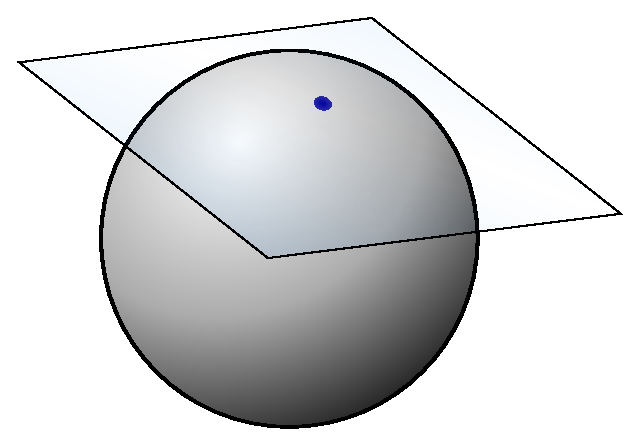
\includegraphics[width=0.4\textwidth]{Image_Tangent-plane}
	\caption{Anschauliche Tangentialebene an $S^2$ in $\R^3$.}
\end{figure}

Eine anschauliche Idee ist wie folgt: Wenn die Mannigfaltigkeit $M$ eingebettet im $\mathbb R^n$ ist, können wir uns in jedem Punkt $p \in M$ eine Tangentialebene vorstellen, in der Tangentialvektoren liegen, die den möglichen Richtungen entsprechen, in die man sich bewegen kann, vgl. Abbildung \ref{fig:tngt_plane}. Hier entsprechen die möglichen Richtungen am Punkt $p$ also Ableitungen von Kurven in $\R^n$, die in der Mannigfaltigkeit verlaufen. Aber wie können wir diese intuitive Idee abstrahieren?

Wir müssen \emph{intrinsisch} über Richtungen in $M$ reden können. Dabei hilft die Beobachtung, dass man das Konzept von Richtungen dazu benutzt, zu beschreiben, wie sich Dinge bei Bewegung in diese Richtung ändern. Die Idee lautet also: Richtung = Richtungsableitung! Wir werden deshalb \glqq Richtungen\grqq\ als Ableitungsoperatoren formalisieren. Dabei ist zum Zwecke der Abstraktion zentral, dass Ableitungen eine Produktregel erfüllen und \glqq lokal\grqq\ wirken.

	Sei im Folgenden $M$ eine differenzierbare Mannigfaltigkeit.

\begin{defn}[Funktionskeime]
	Sei $p \in M$. Auf der Menge $X = \{f \in \sC(U) : U \subset M \text{ offene Umgebung von } p\}$ betrachten wir die Äquivalenzrelation $\sim$, die gegeben ist durch
	\[f \sim g \diff \exists \text{ offene Umgebung } V \text{ von } p \text{ mit } f = g \text{ auf } V.\]
	Die Äquivalenzklassen bzgl. dieser Relation heißen glatte \emph{Funktionskeime} an $M$ im Punkt $p$. Zwei um $p$ definierte Funktionen definieren also genau dann denselben Keim, wenn sie in einer Umgebung von $p$ übereinstimmen.

	Den Raum der Funktionskeime an $M$ in $p$ schreiben wir als $\sC_p(M)$. Den Keim zu einer Funktion $f$ schreiben wir als $[f]$. Wenn keine Missverständnisse entstehen können, schreiben wir stattdessen manchmal auch $f$, um uns Notationsaufwand zu ersparen.
\end{defn}

Zu einem Funktionskeim $[f] \in \sC_p(M)$ ist der Funktionswert $[f](p) := f(p)$ wohldefiniert (warum?).

\begin{prop}
	$\sC_p(M)$ ist mit über die Repräsentanten definierter Addition, Skalarmultiplikation und Multiplikation eine $\mathbb R$-Algebra. \bewUeb
\end{prop}

\begin{defn}
	Eine \emph{Derivation} von $\sC_p(M)$ ist eine lineare Abbildung $v\colon \sC_p(M) \to \mathbb R$, die die \glqq Produktregel\grqq\ \[v(fg) = v(f) g(p) + f(p) v(g)\] erfüllt. Den Raum der Derivationen von $\sC_p(M)$ nennen wir den \emph{Tangentialraum} $T_pM$ an $M$ im Punkt $p$; die Elemente von $T_pM$ heißen auch \emph{Tangentialvektoren} in $p$.

	Der Dualraum von $T_pM$ ist der \emph{Kotangentialraum} $T_p^*M := (T_pM)^*$ an $M$ im Punkt $p$.
\end{defn}

$T_pM$ ist tatsächlich ein Untervektorraum von $(\sC_p(M))^*$ (Übung).

\begin{lemma}[Derivationen verschwinden auf Konstanten]
	Für alle $v \in T_pM$ und $c \in \mathbb R$ ist $v(c) = 0$ (dabei fassen wir $c$ als konstante Funktion bzw. den davon induzierten Funktionskeim auf).
	
	\begin{proof}
		Es ist $v(1) = v(1\cdot 1) = v(1) 1(p) + 1(p) v(1) = 2 v(1)$, also $v(1) = 0$. Da $v$ linear ist, folgt die Behauptung.
	\end{proof}
\end{lemma}

\begin{bsp} \label{bsp:kurve_geschw}
	Sei $I\subset\mathbb R$ offen und $\gamma\colon I \to M$ eine glatte Kurve mit $\gamma(s) = p$ für ein $s \in I$. Wir definieren den Tangentialvektor $\dot\gamma(s) \in T_pM$ durch \[(\dot\gamma(s))(f) := (f\circ\gamma)'(s),\] wobei wir auf der rechten Seite die Ableitung der Funktion $f\circ\gamma \colon I \to \mathbb R, I \subset \mathbb R$ gebildet haben.

	$\dot\gamma(s)$ leitet also die Funktionskeime, auf die es angewendet wird, entlang der Kurve ab; wir können $\dot\gamma(s)$ also als \glqq Geschwindigkeitsvektor\grqq\ der Kurve auffassen. \kommB{Soll dazu noch eine konkrete Rechnung folgen? Vllt. als Übung? (Also dass man konkret im $\R^n$ nachrechnet, dass da so etwas wie eine Richtung herauskommt (unter Identifikation blabla)}

	$\dot\gamma(s)$ ist wohldefiniert und tatsächlich eine Derivation: Wenn $[f] = [g]$ gilt, dann stimmen $f$ und $g$ in einer Umgebung von $p$ überein, und damit stimmen $f\circ\gamma$ und $g\circ\gamma$ in einer Umgebung von $s$ überein und haben insbesondere dieselbe Ableitung an der Stelle $s$. Die Linearität von $\dot\gamma(s)$ folgt aus der Linearität der Ableitung, und die Derivations-Produktregel folgt aus der Produktregel für Ableitungen.
\end{bsp}

Später werden wir sehen, dass sich tatsächlich \emph{jeder} Tangentialvektor als Geschwindigkeitsvektor einer Kurve schreiben lässt.

%%%%%%%%%%%%%%%%%%%%%%%%%%%%%%%%%%%%%%%%%%%%%%%%%%%%%%%%%%%
\section{Das Differential}

Mithilfe des Tangentialraumbegriffs können wir nun nicht nur entscheiden, ob Abbildungen differenzierbar sind, sondern auch tatsächlich eine Art Ableitungsbegriff definieren:
\begin{defn}
	Seien $M,N$ differenzierbare Mannigfaltigkeiten und $f\colon M \to N$ eine glatte Abbildung. Das \emph{Differential} von $f$ im Punkt $p\in M$ ist die lineare Abbildung
	\[\left.\DD f\right|_p \colon T_pM \to T_{f(p)}N\]
	definiert durch
	\[\left(\left.\DD f\right|_p(v)\right)(\alpha) = v (\alpha\circ f)\]
	für $v\in T_pM, \alpha \in \sC_{f(p)}(N)$.
\end{defn}
\begin{prop}
	$\left.\DD f\right|_p(v)$ ist tatsächlich wohldefiniert und eine Derivation von $\sC_{f(p)}(N)$, und $\left.\DD f\right|_p$ ist linear. \bewUeb
\end{prop}

\begin{bem}
	Ist $\gamma\colon I \to M$ eine glatte Kurve und $f\colon M \to N$ glatt, so ist $\tilde\gamma := f\circ\gamma \colon I \to N$ eine Kurve in $M$. Der Geschwindigkeitsvektor von dieser Kurve zum Zeitpunkt $s$ ist $\dot{\tilde\gamma}(s) = \left.\DD f\right|_{\gamma(s)} (\dot\gamma(s))$ (Übung!).
	
	Wenn wir uns auf $M$ also vom Punkt $\gamma(s)$ aus in Richtung $v := \dot\gamma(s)$ bewegen, dann bewegt sich unser Bild unter $f$ auf $N$ also in Richtung $\left.\DD f\right|_p(v)$. Das Differential beschreibt also in einem sinnvollen Sinne, wie sich \glqq Richtungen\grqq\ unter Abbildungen zwischen Mannigfaltigkeiten verhalten.
\end{bem}

\begin{satz}[Kettenregel]
	Seien $f\colon M \to N, g\colon N \to L$ glatte Abbildungen zwischen differenzierbaren Mannigfaltigkeiten, und $p \in M$. Dann gilt \[\left.\DD(g\circ f)\right|_p = \left.\DD g\right|_{f(p)} \circ \left.\DD f\right|_p.\]

	\begin{proof}
		Sei $v \in T_pM$. Für jedes $\alpha \in \sC_{g(f(p))}(L)$ ist
		\begin{align*}
			\left(\left.\DD(g\circ f)\right|_p(v)\right)(\alpha) &= v(\alpha\circ (g \circ f))\\
			&= v((\alpha\circ g) \circ f)\\
			&= \left(\left.\DD f\right|_p(v)\right) (\alpha \circ g)\\
			&= \left(\left.\DD g\right|_{f(p)} \left(\left.\DD f\right|_p(v)\right)\right) (\alpha),
		\end{align*}
		also gilt $\left.\DD(g\circ f)\right|_p(v) = \left.\DD g\right|_{f(p)}\left(\left.\DD f\right|_p(v)\right)$.
	\end{proof}
\end{satz}

\begin{lemma} \label{lemma:differential_diffeo}
	\begin{enumerate}[label=(\alph*)]
		\item $\left.\DD(\id_M)\right|_p = \id_{T_pM}$
		\item Ist $f\colon M \to N$ ein Diffeomorphismus, so ist $\left.\DD f\right|_p$ für jedes $p\in M$ ein Isomorphismus, und es gilt $\left.\DD f^{-1}\right|_{f(p)} = \left(\left.\DD f\right|_p\right)^{-1}$.
	\end{enumerate}
	\bewUeb
\end{lemma}

\begin{prop}
	Sei $M$ eine differenzierbare Mannigfaltigkeit und $U\subset M$ eine offene Teilmenge. Für jedes $p\in U$ ist $T_pU$ kanonisch isomorph zu $T_pM$ vermöge $\left.\DD i\right|_p$, wobei $i\colon U \to M, i(q) := q$ die Inklusionsabbildung ist.

	\begin{proof}
		Sei $p \in U$. $\left.\DD i\right|_p$ ist definiert über $\left(\left.\DD i\right|_p(v)\right)(\alpha) = v(\alpha\circ i)$ für $v \in T_pU$ und $\alpha \in \sC_p(M)$; d.\,h. $\left.\DD i\right|_p(v)$ ist einfach $v$, nur aufgefasst als Derivation, die Funktionskeime an $M$ ableitet, indem man diese als Funktionskeime an $U$ auffasst. Da Funktionskeime an $U$ in $p$ und Funktionskeime an $M$ in $p$ aber einander entsprechen, ist damit klar, dass $\left.\DD i\right|_p$ ein Isomorphismus ist.

		Etwas genauer: Jeder Funktionskeim $\tilde\alpha \in \sC_p(U)$ kann auch als Keim $\alpha \in \sC_p(M)$ aufgefasst werden, und umgekehrt: Jede offene Umgebung von $p$ in $U$ ist auch offen in $M$, und jede offene Umgebung von $p$ in $M$ enthält eine offene Umgebung von $p$ in $U$. Da bei der Definition von Funktionskeimen um $p$ Funktionen äquivalent sind, wenn sie auf einer offenen Umgebung von $p$ übereinstimmen, spielt es also keine Rolle, ob wir in $U$ oder in $M$ sind (\glqq es wird eh alles äquivalent gemacht\grqq)\footnote{
			Als Element von $\sC_p(M)$ besteht der Keim / die Äquivalenzklasse potentiell aus mehr Funktionen, da auch noch Funktionen dazukommen, die auf \glqq größeren\grqq\ Umgebungen von $p$ definiert sind.
		}.

		Diese Abbildung $\sC_p(M) \ni \alpha \mapsto \tilde\alpha \in \sC_p(U)$ ist also für $[f]_{p,M} \in \sC_p(M)$, $f$ definiert auf $V$, gegeben durch $[f]_{p,M} \mapsto \left[\left.f\right|_{U\cap V}\right]_{p,U} \in \sC_p(U)$, was man auch schreiben kann als $[f]_{p,M} \mapsto \left[\left.f\circ i\right|_{U\cap V}\right]_{p,U}$. D.\,h. das oben beschriebene Auffassen von $\alpha$ als Keim auf der kleineren Mannigfaltigkeit $U$ ist die Abbildung $\sC_p(M) \ni \alpha \mapsto \alpha\circ i \in \sC_p(U)$. Wie oben beschrieben lässt sich das umkehren, ist also ein Isomorphismus. Damit ist aber auch $\left.\DD i\right|_p$ ein Isomorphismus, denn es ist definiert als $\left(\left.\DD i\right|_p(v)\right)(\alpha) = v(\alpha\circ i)$.
	\end{proof}
\end{prop}

Da $\left.\DD i\right|_p(v)$ einfach dieselbe Derivation wie $v$ ist (sie unterscheiden sich nur darin, ob man die Keime, auf die sie wirkt, als Keime an $M$ oder an $U$ betrachtet), werden wir im Folgenden $T_pU$ und $T_pM$ (meistens) miteinander identifizieren.

%%%%%%%%%%%%%%%%%%%%%%%%%%%%%%%%%%%%%%%%%%%%%%%%%%%%%%%%%%%
\section{Der Tangentialraum eines Vektorraums}

Betrachten wir einen endlich-dimensionalen Vektorraum $V$, so sagt uns die Intuition, dass die Richtungen, in die wir ableiten können, einfach die Richtungen des Vektorraums sein sollten. Wir erwarten also einen kanonischen Isomorphismus $T_pV \cong V$ für alle $p \in V$. Sei im Folgenden $V$ ein endlich-dimensionaler Vektorraum und $p \in V$ ein fester Punkt.
\begin{defn}
	Für $v \in V$ definieren wir den Tangentialvektor $\left.\partial_v\right|_p \in T_pV$ durch
	\[\left.\partial_v\right|_p(f) := (\partial_v f)(p) = \left.\frac{\D f(p + h v)}{\D h}\right|_{h=0} = \lim_{h\to 0} \frac{f(p + h v) - f(p)}{h}.\]
\end{defn}
$\left.\partial_v\right|_p$ ist also einfach die Richtungsableitung in Richtung von $v$ am Punkt $p$.
\begin{prop}
	$\left.\partial_v\right|_p$ ist tatsächlich eine Derivation von $\sC_p(V)$.
	
	\begin{proof}
		$\left.\partial_v\right|_p$ ist wohldefiniert, denn wenn $[f] = [g]$ gilt, dann stimmen $f$ und $g$ in einer Umgebung von $p$ überein und haben insbesondere dieselben Ableitungen an der Stelle $p$. Dass Richtungsableitungen linear sind und die Produktregel erfüllen, ist bekannt\footnote{Oder folgt schnell aus den entsprechenden Eigenschaften für Ableitungen von Funktionen $\mathbb R \to \mathbb R$.}.
	\end{proof}
\end{prop}

\begin{satz} \label{satz:tangt_vr}
	Die Abbildung \[V \to T_pV, v \mapsto \left.\partial_v\right|_p\] ist ein linearer Isomorphismus.
	
	\begin{proof}\let\qed\relax
		Linearität ist einfach zu zeigen (Übung). Um Surjektivität und Injektivität zu zeigen, fixieren wir eine Basis $\{b_1,\dots,b_n\}$ von $V$. Sei $\{\theta^1, \dots, \theta^n\}$ die dazu duale Basis von $V^*$, also für $i = 1, \dots, n$ jeweils $\theta^i\colon V \to \mathbb R$ die lineare Abbildung definiert durch $\theta^i(b_j) = \delta^i_j$ und lineare Fortsetzung.

		Für beliebiges $v = \sum_{i=1}^n v^i b_i \in V$ ist
		\begin{equation} \label{eq:pf_tangt_vr}
			\left.\partial_v\right|_p(\theta^i) = \left.\frac{\D\theta^i(p + h v)}{\D h}\right|_{h=0} = \left.\frac{\D(\theta^i(p) + h v^i)}{\D h}\right|_{h=0} = v^i
		\end{equation}
		für alle $i$. Falls $\left.\partial_v\right|_p = 0$ gilt, ist also $v^i = \left.\partial_v\right|_p(\theta^i) = 0(\theta^i) = 0$, also $v=0$. Das zeigt, dass der Kern der betrachteten Abbildung nur die 0 enthält, also deren Injektivität. Um die Surjektivität zu zeigen, brauchen wir einen kleinen Trick.
	\end{proof}
\end{satz}

\begin{lemma}[Hadamard-Lemma] \label{lemma:Hadamard}
	Seien $U \subset \mathbb R^n$ eine offene Menge, die sternförmig um $x_0$ ist, und $f \in \sC(U)$. Dann gibt es glatte Funktionen $f_i \in \sC(U), i = 1,\dots,n$, sodass \[f(x) = f(x_0) + \sum_{i=1}^n f_i(x) (x^i - x_0^i).\]
	
	\begin{proof}
		Für $x \in U$ setze $y := x - x_0$. Dann ist
		\begin{align*}
		f(x) - f(x_0) &= f(x_0 + 1\cdot y) - f(x_0 + 0\cdot y)\\
		&= \int_0^1 \left(\frac{\D}{\D t} f(x_0 + ty)\right) \D t\\
		\text{(Kettenregel)} \quad &= \int_0^1 \sum_{i=1}^n (\partial_i f)(x_0 + ty) y^i \D t\\
		&= \sum_{i=1}^n \left(\int_0^1 (\partial_i f)(x_0 + tx - tx_0) \D t\right) (x^i - x_0^i).
		\end{align*}
		Mit \[f_i(x) := \int_0^1 (\partial_i f)(x_0 + tx - tx_0) \D t\] folgt also die Behauptung (die $f_i$ sind glatt wegen Kettenregel und Sätzen über das Differenzieren unter dem Integral).
	\end{proof}
\end{lemma}

\begin{kor}[Hadamard-Lemma auf Vektorräumen]
	Sei $\theta = (\theta^1, \dots, \theta^n) \colon V \to \mathbb R^n$ ein linearer Isomorphismus und sei $\alpha \in \sC_p(V)$. Dann gibt es $\alpha_i \in \sC_p(V), i = 1,\dots, n$ mit \[\alpha = \alpha(p) + \sum_{i=1}^n \alpha_i \cdot (\theta^i - \theta^i(p)).\]
	
	\begin{proof}
		Das ist einfach das Hadamard-Lemma \ref{lemma:Hadamard} angewendet auf unseren Vektorraum $V$, der über $\theta$ mit $\mathbb R^n$ identifiziert wurde.
	\end{proof}
\end{kor}

\begin{proof}[Zurück zum Beweis von Satz \ref{satz:tangt_vr}]
	Mit dem Hadamard-Lemma können wir jetzt auch zeigen, dass die Abbildung $v \mapsto \left.\partial_v\right|_p$ surjektiv ist. Seien $w \in T_pV$ und $\alpha \in \sC_p(V)$ beliebig, und seien $\alpha_i \in \sC_p(V)$ zu $\alpha$ mit dem Hadamard-Lemma gewählt. Dann ist
	\begin{align}\begin{split}
		w(\alpha) &= w\left(\alpha(p) + \sum_{i=1}^n \alpha_i \cdot (\theta^i - \theta^i(p))\right)\\
		\text{(Linearität, $w(\text{const.}) = 0$)} \quad &= \sum_{i=1}^n w(\alpha_i \cdot (\theta^i - \theta^i(p)))\\
		&= \sum_{i=1}^n \left( w(\alpha_i) \cdot (\theta^i(p) - \theta^i(p)) + \alpha_i(p) \cdot w(\theta^i) \right)\\
		&= \sum_{i=1}^n \alpha_i(p) \cdot w(\theta^i).
	\end{split}\end{align}
	Insbesondere gilt damit auch $\left.\partial_v\right|_p (\alpha) = \sum_{j=1}^n \alpha_i(p) \cdot \left.\partial_v\right|_p (\theta^i) \overset{\eqref{eq:pf_tangt_vr}}{=} \sum_{j=1}^n \alpha_i(p) \cdot v^i$ für beliebige Vektoren $v = \sum_{i=1}^n v^i b_i$. Wir können also $w(\alpha) = \left.\partial_v\right|_p (\alpha)$ erreichen, indem wir $v := \sum_{i=1}^n w(\theta^i) b_i$ setzen.

	Da $\alpha$ beliebig war, gilt also $w = \left.\partial_v\right|_p$. Wir können also jedes $w \in T_pV$ als Richtungsableitung in Richtung eines Vektors $v\in V$ schreiben.
\end{proof}

Der Tangentialraum $T_pV$ an einen endlich-dimensionalen Vektorraum $V$ ist also in kanonischer Weise zu $V$ selbst isomorph; ein Vektor $v \in V$ wird dabei mit der Richtungsableitung $\left.\partial_v\right|_p$ identifiziert.

Bzgl. dieser Identifikation ist der in Beispiel \ref{bsp:kurve_geschw} definierte abstrakte \glqq Geschwindigkeitsvektors\grqq\ einer Kurve identisch zur üblichen Ableitung der Kurve als vektorwertige Funktion:
\begin{lemma}
	Sei $I\subset \R$ eine offene Menge, $s\in I$, $\gamma\colon I\to V$ eine Kurve und $p := \gamma(s)$.

	Von dieser Kurve können wir einerseits die übliche Ableitung
	\[\gamma'(s) = \lim_{h\to 0} \frac{\gamma(s+h) - p}{h} \in V\]
	bilden; andererseits können wir den abstrakten Geschwindigkeitsvektor $\dot\gamma(s) \in T_pV$ bilden.

	Bzgl. der kanonischen Identifikation $V \equiv T_pV$ ist dann $\gamma'(s) \equiv \dot\gamma(s)$.

	\begin{proof}
		Übung. (Tipp: Verwende die mehrdimensionale Kettenregel für vektorwertige Abbildungen!)
	\end{proof}
\end{lemma}

\begin{kor}
	Auf dem $\mathbb R^n$ bilden die partiellen Ableitungsoperatoren $\left.\partial_1\right|_p, \dots, \left.\partial_n\right|_p$ eine Basis des Tangentialraums $T_p\mathbb R^n$.

	\begin{proof}
		$\left.\partial_i\right|_p$ ist die Richtungsableitung in Richtung des Standardbasisvektors $\e_i$.
	\end{proof}
\end{kor}

\begin{kor} \label{kor:entw_tangt_Rn}
	Die Entwicklung eines Tangentialvektors $w \in T_p\mathbb R^n$ in dieser Basis ist
	\[w = \sum_{i=1}^n w(\pr^i) \left.\partial_i\right|_p,\]
	wobei $\pr^i\colon \mathbb R^n \to \mathbb R, \pr^j(a) = a^j$ die Projektion auf die $i$-te Komponente ist.

	\begin{proof}
		Das ergibt sich direkt aus dem Beweis von Satz \ref{satz:tangt_vr}, da die Projektionen $\pr^i$ die zu $\e_i$ duale Basis von $(\mathbb R^n)^*$ bilden.
	\end{proof}
\end{kor}

\begin{bsp}
	Ist $U\subset\mathbb R^n$ offen und $p\in U$, so bilden die partiellen Ableitungsableitungen $\left.\partial_1\right|_p, \dots, \left.\partial_n\right|_p$ eine Basis von $T_pU$ (denn es ist ja $T_pU = T_p\mathbb R^n$).
\end{bsp}

\begin{satz}[Differential von linearen Abbildungen]
	Sei $L\colon V \to W$ eine lineare Abbildung. Bzgl. der Identifikationen $T_pV \equiv V, T_{L(p)}W \equiv W$ ist $\left.\DD L\right|_p = L$.

	\begin{center}
		\begin{tikzpicture}
		\matrix(m)[matrix of math nodes,row sep=4em,column sep=4em,minimum width=2em]{T_pV & T_{L(p)}W \\
			V&W \\};
		\path[-stealth]
		(m-1-1)	edge node [above]{$\left.\DD L\right|_p$} (m-1-2)
		(m-2-1) edge node [left]{$v \mapsto \left.\partial_v\right|_p$} (m-1-1)
		(m-2-2) edge node [right]{$w \mapsto \left.\partial_w\right|_{L(p)}$} (m-1-2)
		(m-2-1) edge node [above]{$L$} (m-2-2)
		;
		\end{tikzpicture}
	\end{center}

	\begin{proof}
		Für $v\in V$ ist
		\begin{align*}
			\left(\left.\DD L\right|_p \left( \left.\partial_v\right|_p \right)\right) (f) &= \left.\partial_v\right|_p (f \circ L)\\
			&= \left.\frac{\D f(L(p + h v))}{\D h}\right|_{h=0}\\
			&= \left.\frac{\D f(L(p) + h L(v))}{\D h}\right|_{h=0}\\
			&= \left.\partial_{L(v)}\right|_{L(p)} (f)
		\end{align*}
		für beliebige $f$, also $\left.\DD L\right|_p \left( \left.\partial_v\right|_p \right) = \left.\partial_{L(v)}\right|_{L(p)}$.
		Das mussten wir aber zeigen.
	\end{proof}
\end{satz}

\begin{bsp} \label{bsp:abl_kurve_differential}
	Sei $I \subset \mathbb R$ eine offene Menge, $s \in I$ und $\left.\partial_1\right|_s$ der kanonische Ableitungsoperator, der eine Basis von $T_s I$ bildet.

	Ist $M$ eine differenzierbare Mannigfaltigkeit und $\gamma\colon I \to M$ eine glatte Kurve, so können wir das Differential $\left.\DD \gamma\right|_s \colon T_sI \to T_{\gamma(s)} M$ betrachten. Dieses bildet den Basisvektor $\left.\partial_1\right|_s$ ab auf die Derivation $\left.\DD \gamma\right|_s(\left.\partial_1\right|_s)$, die wirkt als $\left(\left.\DD \gamma\right|_s(\left.\partial_1\right|_s)\right)(f) = \left.\partial_1\right|_s (f\circ\gamma) = \left.\frac{\D(f\circ\gamma)(s + h)}{\D h}\right|_{h=0} = (f\circ\gamma)'(s)$. Das ist aber genau die Wirkung des in Beispiel \ref{bsp:kurve_geschw} definierten \glqq Geschwindigkeitsvektors\grqq\ $\dot\gamma(s) \in T_{\gamma(s)} M$, also gilt $\left.\DD \gamma\right|_s(\left.\partial_1\right|_s) = \dot\gamma(s)$.

	Der \glqq Geschwindigkeitsvektor\grqq\ $\dot\gamma(s)$ ist also tatsächlich in einem formalen Sinne die Ableitung der Kurve $\gamma$ an der Stelle $s$, nämlich das Differential von $\gamma$ an dieser Stelle angewendet auf den kanonischen Basisvektor von $T_sI$.
\end{bsp}

\begin{lemma}[Differential von glatten Funktionen als Anwendung der Derivation]
	Für $f\in\sC(M)$ und $v \in T_pM$ ist $\left.\DD f\right|_p(v) = v(f)$ unter der kanonischen Identifikation $T_{f(p)}\mathbb R \equiv \mathbb R$.

	\begin{proof}
		Nach Korollar \ref{kor:entw_tangt_Rn} ist $\left.\DD f\right|_p(v) = \Big(\DD f\big|_p(v)\Big)(\id) \cdot \left.\partial_1\right|_{f(p)} \in T_{f(p)}\mathbb R$. Da nach Definition $\Big(\DD f\big|_p(v)\Big)(\id) = v(\id \circ f) = v(f)$ gilt und $\left.\partial_1\right|_{f(p)}$ unter $T_{f(p)}\mathbb R \equiv \mathbb R$ mit $1$ identifiziert wird, folgt die Behauptung.
	\end{proof}
\end{lemma}

\begin{defn}
	Fassen wir für $f \in \sC(M)$ das Differential $\left.\DD f\right|_p$ wie oben als Abbildung nach $\mathbb R$ auf, so schreiben wir es als $\left.\D f\right|_p \colon T_pM \to \mathbb R$, also $\left.\D f\right|_p \in T_p^*M$.
\end{defn}

%%%%%%%%%%%%%%%%%%%%%%%%%%%%%%%%%%%%%%%%%%%%%%%%%%%%%%%%%%%
\section{Koordinatenvektoren}

Haben wir auf einer Mannigfaltigkeit $M$ eine Karte $(x,U)$ gegeben, dann ermöglicht sie uns, $U$ mit einer offenen Teilmenge des $\mathbb R^n$ zu identifizieren. Das gilt auch für die Tangentialräume:
\begin{defn}
	Sei $M$ eine differenzierbare Mannigfaltigkeit, $p\in M$ und $(x,U)$ eine Karte um $p$. Wir schreiben $V = x(U) \subset \mathbb R^n$. Als Abbildung $x\colon U \to V$ ist $x$ ein Diffeomorphismus (Übung!). Nach Lemma \ref{lemma:differential_diffeo} ist dann also
	\[\left.\DD x\right|_p \colon T_pM \to T_{x(p)} \mathbb R^n\]
	ein Isomorphismus, wobei wir die Identifikationen $T_pM = T_pU$, $T_{x(p)}\mathbb R^n = T_{x(p)} x(U)$ benutzt haben. Diesen benutzen wir, um aus der kanonischen Basis $\{\left.\partial_i\right|_{x(p)}\}$ von $T_{x(p)}\mathbb R^n$ eine Basis von $T_pM$ zu erhalten: Für $i = 1,\dots, n$ definieren wir
	\[\left.\frac{\partial}{\partial x^i}\right|_p := \left(\left.\DD x\right|_p\right)^{-1} \left(\left.\partial_i\right|_{x(p)}\right) = \left.\DD x^{-1}\right|_{x(p)} \left(\left.\partial_i\right|_{x(p)}\right)\]
	Die $\left.\frac{\partial}{\partial x^i}\right|_p$ heißen die von $x$ \emph{induzierten Koordinatenvektoren} in $p$, zusammen bilden sie die von $x$ induzierte \emph{Koordinatenbasis} von $T_pM$.
\end{defn}
Die Koordinatenvektoren wirken durch
\[\left.\frac{\partial}{\partial x^i}\right|_p(f) = \left.\partial_i\right|_{x(p)} (f \circ x^{-1}) = \left(\partial_i (f\circ x^{-1})\right) (x(p)).\]
$\left.\frac{\partial}{\partial x^i}\right|_p$ stellt also einen Funktionskeim in der Karte $x$ dar und bildet die $i$-te partielle Ableitung dieser Kartendarstellung.

\begin{bem}
	Wenn wir in Koordinaten rechnen wollen, schreiben wir Karten meist als $x = (x^1, \dots, x^n)$ o.\,ä. statt als $\varphi$ o.\,ä., da das zur historisch etablierten Notation von Koordinatenvektoren passt. Die Funktionen $x^i$ nennt man dann auch \emph{Koordinatenfunktionen}, die $x^i(p)$ sind die \emph{Koordinaten} von $p$.

	Aufpassen muss man dann allerdings manchmal, wenn man Punkte im $\mathbb R^n$ auch als $x$ schreibt (deshalb haben wir das oben auch eher vermieden).
\end{bem}

\begin{bsp}
	Für eine Karte $(x,U)$ um $p$ sind die Komponenten $x^i, i = 1,\dots, n$ reellwertige glatte Funktionen auf $U$, können also als Funktionskeime in $p$ aufgefasst werden. Wendet man darauf die Koordinatenvektoren an, so erhält man
	\begin{align*}
		\left.\frac{\partial}{\partial x^i}\right|_p (x^j) &= \left(\partial_i \left(x^j\circ x^{-1}\right)\right) (x(p))\\
		&= \underbrace{\left(\partial_i \pr^j\right)}_{= \delta^j_i} (x(p)) = \delta^j_i,
	\end{align*}
	wobei $\pr^j\colon \mathbb R^n \to R, \pr^j(a) = a^j$ die Projektion auf die $j$-te Komponente ist.
\end{bsp}
Für die Kovektoren $\left.\D x^i\right|_p \in T_p^*M$ gilt also $\left.\D x^i\right|_p\left(\left.\frac{\partial}{\partial x^j}\right|_p\right) = \delta^i_j$. Damit haben wir gezeigt:
\begin{lemma}
	Die zur von $x$ induzierten Koordinatenbasis von $T_pM$ duale Basis von $T_p^*M$ ist gegeben durch die Differentiale $\left\{\left.\D x^i\right|_p \right\}$. \qed
\end{lemma}

\begin{lemma}[Koordinatendarstellung von Tangentialvektoren]
	Sei $M$ eine differenzierbare Mannigfaltigkeit, $p \in M$, $v \in T_pM$ und $x$ eine Karte um $p$. Die Darstellung von $v$ in der von $x$ induzierten Koordinatenbasis ist
	\[v = \sum_{i=1}^n v^i \left.\frac{\partial}{\partial x^i}\right|_p\]
	mit
	\[v^i = v(x^i).\]

	\begin{proof}
		Nach Korollar \ref{kor:entw_tangt_Rn} lässt sich $\left.\DD x\right|_p(v) \in T_{x(p)}\R^n$ schreiben als $\left.\DD x\right|_p(v) = \sum_{i=1}^n \Big(\DD x\big|_p(v)\Big) (\pr^i) \left.\partial_i\right|_{x(p)}$. Da nach Definition $\Big(\DD x\big|_p(v)\Big) (\pr^i) = v(\pr^i \circ x) = v(x^i)$ ist, haben wir also $\left.\DD x\right|_p(v) = \sum_{i=1}^n v(x^i) \left.\partial_i\right|_{x(p)}$.
		Anwenden von $\left(\left.\DD x\right|_p\right)^{-1}$ auf beiden Seiten liefert die Behauptung.
	\end{proof}
\end{lemma}

\begin{nota}[Einstein'sche Summenkonvention]
	Da bei Rechnungen in Koordinaten oder bzgl. Basen oft Summen der Form
	\[\sum_{i=1}^n v^i b_i\]
	auftreten, vereinbaren wir, um die Notation zu verkürzen, dass in Zukunft bei solchen Summationen das Summenzeichen weggelassen werden kann; stattdessen schreiben wir in Zukunft also
	\[v^i b_i.\]
	Immer, wenn in einem Term ein Index zweimal vorkommt, einmal oben an einem Symbol und einmal unten, wird dieser Term über alle im jeweiligen Kontext möglichen Werte des Index aufsummiert. Ein komplizierteres Beispiel für einen Ausdruck in Summenkonvention und seine Bedeutung ist
	\[T^{ij}_{kl} S^k_j v^l b_i = \sum_{i,j,k,l = 1}^n T^{ij}_{kl} S^k_j v^l b_i.\]

	Die Komponenten von Tangentialvektoren schreiben wir mit oberen Indizes, Basisvektoren des Tangentialraums dementsprechend mit unteren Indizes. Einen oberen Index, der wie in $\left.\frac{\partial}{\partial x^i}\right|_p$ \glqq im Nenner\grqq\ steht, fassen wir dementsprechend als unteren Index auf.

	Mit Summenkonvention lautet die obigen Entwicklungsformel also
	\[v = v(x^i) \left.\frac{\partial}{\partial x^i}\right|_p.\]
\end{nota}

\begin{lemma}[Differential in Kartendarstellung] \label{lemma:differential_koord}
	Sei $f\colon M \to N$ eine glatte Abbildung zwischen differenzierbaren Mannigfaltigkeiten. Sei $p\in M$, $x$ eine Karte von $M$ um $p$ und $y$ eine Karte von $N$ um $f(p)$. Dann ist die Darstellungsmatrix des Differentials $\left.\DD f\right|_p$ bzgl. der Koordinatenbasen $\left.\frac{\partial}{\partial x^i}\right|_p$ von $T_pM$ und $\left.\frac{\partial}{\partial y^i}\right|_{f(p)}$ von $T_{f(p)}N$ die Jacobi-Matrix der Kartendarstellung $y \circ f \circ x^{-1}$ von $f$ an der Stelle $x(p)$, also die Matrix
	\[\mathrm{J}(y\circ f\circ x^{-1})|_{x(p)} = \left[\left(\partial_j(y\circ f\circ x^{-1})^i\right) (x(p)) \right]_{ij}.\]
	\bewUeb
\end{lemma}

\begin{defn}
	Sei $M$ eine differenzierbare Mannigfaltigkeit und $(x,U)$ eine Karte. Für $f \in \sC(U)$ definieren wir die Funktionen $\frac{\partial f}{\partial x^i} \in \sC(U)$ durch
	\[\frac{\partial f}{\partial x^i}(p) := \left.\frac{\partial}{\partial x^i}\right|_p(f).\]
	Manchmal nennen wir diese Funktionen die \emph{partiellen Ableitungen} von $f$ bzgl. der Karte $x$, wobei das natürlich \emph{abuse of language} ist.
\end{defn}

Mit dieser Notation ist die Darstellungsmatrix des Differentials aus Lemma \ref{lemma:differential_koord} also
\[\left[\frac{\partial(y^i \circ f)}{\partial x^j}(p)\right]_{ij}.\]

\begin{satz}[Satz von der inversen Abbildung]
	Sei $f\colon M \to N$ eine glatte Abbildung zwischen differenzierbaren Mannigfaltigkeiten. Ist $\left.\DD f\right|_p\colon T_pM \to T_{f(p)}N$ ein Isomorphismus, dann ist $f$ ein lokaler Diffeomorphismus um $p$, d.\,h. es gibt eine offene Umgebung $U\subset M$ von $p$, sodass $f|_U \colon T \to f(U)$ ein Diffeomorphismus ist.

	\begin{proof}
		Das folgt mit Lemma \ref{lemma:differential_koord}, indem man den Satz von der inversen Abbildung für Abbildungen zwischen Teilmengen des $\R^n$ auf die Kartendarstellung von $f$ anwendet.
	\end{proof}
\end{satz}

\begin{lemma}[Transformationsformel für Tangentialvektoren]
	Sei $M$ eine differenzierbare Mannigfaltigkeit, $p\in M$ und seien $x, \tilde x$ zwei Karten um $p$. Für die Koordinatenvektoren gilt
	\[\left.\frac{\partial}{\partial \tilde x^i}\right|_p = \frac{\partial x^j}{\partial \tilde x^i}(p) \left.\frac{\partial}{\partial x^j}\right|_p.\]
	Die Basiswechselmatrix ist also die Jacobi-Matrix des inversen Kartenwechsels $x \circ \tilde x^{-1}$ (an der Stelle $\tilde x(p)$).

	Für einen Tangentialvektor $v = v^i \left.\frac{\partial}{\partial x^i}\right|_p = \tilde v^i \left.\frac{\partial}{\partial \tilde x^i}\right|_p$ gilt dementsprechend
	\[\tilde v^j = \frac{\partial \tilde x^j}{\partial x^i}(p) v^i.\]

	\bewUeb
\end{lemma}

%%%%%%%%%%%%%%%%%%%%%%%%%%%%%%%%%%%%%%%%%%%%%%%%%%%%%%%%%%%
\section{Ableitungen von Kurven}
\begin{bem}
	Für eine offene Menge $I\subset\mathbb R$ schreibt man die kanonische Karte $\id_I\colon I \to I$ oft als $t$ und den davon induzierten Koordinatenvektor dann als $\left.\frac{\D}{\D t}\right|_s \in T_sI$. Das ist natürlich einfach der normale Ableitungsoperator an der Stelle $s$, den wir oben schon als $\left.\partial_1\right|_s$ geschrieben haben. Für eine glatte Kurve $\gamma\colon I \to M$ ist also (vgl. Beispiel \ref{bsp:abl_kurve_differential})
	\[\dot\gamma(s) = \left.\DD\gamma\right|_s \left(\left.\frac{\D}{\D t}\right|_s\right).\]

	Statt $\dot\gamma(s)$ schreiben wir für die Ableitung einer Kurve an der Stelle $s$ in Zukunft auch
	\[\dot\gamma(s) = \left.\frac{\D}{\D t}\gamma(t)\right|_{t = s}.\]

	Man kann sich überlegen, dass
	\[\dot\gamma(s) = \left.\frac{\D}{\D t}\gamma(s + t)\right|_{t = 0}\]
	gilt (Übung!).
\end{bem}
Mit dieser Schreibweise nimmt die Identifikation eines endlich-dimensionalen Vektorraums mit seinem Tangentialraum eine sehr suggestive Form an:
\begin{lemma}
	Sei $V$ ein endlich-dimensionaler Vektorraum und $p, v\in V$. Die Identifikation $V \equiv T_pV$ lässt sich schreiben als
	\[V \ni v \equiv \left.\frac{\D}{\D t}(p + tv)\right|_{t=0} \in T_pV.\]
	\bewUeb
\end{lemma}

Die folgende Form der Kettenregel ist oft sehr hilfreich.
\begin{lemma}[Kettenregel für Ableitungen von Kurven]
	Sei $I \subset\R$ eine offene Umgebung von 0, $\gamma\colon I \to M$ eine glatte Kurve und $f\colon M \to N$ eine glatte Abbildung. Dann gilt
	\[\left.\frac{\D}{\D t}f(\gamma(t))\right|_{t=0} = \left.\DD f\right|_{\gamma(0)} \left(\left.\frac{\D}{\D t}\gamma(t)\right|_{t=0}\right).\]

	\begin{proof}
		Mit der obigen Bemerkung folgt das direkt aus der Kettenregel.
	\end{proof}
\end{lemma}

\begin{lemma}[Koordinatenvektoren sind Ableitungen von Koordinatenlinien]
	Sei $M$ eine differenzierbare Mannigfaltigkeit und $(x,U)$ eine Karte um $p$. Sei $i \in \{1,\dots,n\}$.

	Für genügend kleine $t$ liegt $x(p) + t \e_i$ in $x(U) \subset \R^n$, d.\,h. $t \mapsto x^{-1}(x(p) + t\e_i)$ ist eine Kurve durch $p$ in $U$. Dies ist gerade die \emph{$i$-te Koordinatenlinie} durch $p$, d.\,h. die Kurve durch $p$, entlang derer die Koordinate $x^i$ variiert und die anderen Koordinaten $x^j, j\ne i$ konstant bleiben.

	Die Ableitung dieser Koordinatenlinie ist der $i$-te Koordinatenvektor,
	\[\left.\frac{\D}{\D t} x^{-1}(x(p) + t\e_i) \right|_{t=0} = \left.\frac{\partial}{\partial x^i}\right|_p.\]

	\bewUeb
\end{lemma}
Damit kann man jetzt sehr leicht zeigen, dass jeder Tangentialvektor sich als Ableitung einer Kurve schreiben lässt.
\begin{lemma}
	Sei $M$ eine differenzierbare Mannigfaltigkeit und $p\in M$. Jeder Tangentialvektor $v\in T_pM$ ist Ableitung einer Kurve.

	\bewUeb
\end{lemma}


%%%%%%%%%%%%%%%%%%%%%%%%%%%%%%%%%%%%%%%%%%%%%%%%%%%%%%%%%%%
\chapter{Multilineare Algebra: Das Tensorprodukt}
\epigraph{Mathematics is the art of giving the same name to different things.}
{\textsc{Henri Poincaré}}

%%%%%%%%%%%%%%%%%%%%%%%%%%%%%%%%%%%%%%%%%%%%%%%%%%%%%%%%%%%
\section{Das Tensorprodukt von Vektorräumen}
\begin{defn} \label{defn:tensor_prod}
	Seien $V,W$ zwei Vektorräume.
	\begin{enumerate}[label=(\alph*)]
		\item Das \emph{Tensorprodukt} $V\otimes W$ ist ein Vektorraum, der wie folgt definiert wird:

			Die Elemente von $V\otimes W$ sind formale Summen von formalen Ausdrücken der Form $v\otimes w$ mit $v\in V, w\in W$, d.\,h.
			\[V\otimes W = \left\{\sum_{i=1}^k v_i \otimes w_i : k\in\mathbb N, v_i \in V, w_i \in W\right\}.\]
			Die formalen Ausdrücke haben dabei genau die folgenden Eigenschaften:
			\begin{enumerate}[label=(\roman*)]
				\item $v \otimes (w + \tilde w) = v\otimes w + v \otimes \tilde w$ für alle $v \in V$ und $w, \tilde w \in W$
				\item $(v + \tilde v) \otimes w = v\otimes w + \tilde v \otimes w$ für alle $v, \tilde v \in V$ und $w \in W$
				\item $(\lambda v) \otimes w = v \otimes (\lambda w)$ für alle $v\in V, w\in W, \lambda \in \R$
			\end{enumerate}
			Das \glqq genau\grqq\ bedeutet dabei, dass zwei Ausdrücke, die nicht mithilfe dieser Eigenschaften ineinander umgeformt werden können, auch wirklich verschieden sind.

			Wir definieren auf $V\otimes W$ eine Skalarmultiplikation durch
			\[\lambda\left(\sum_{i=1}^k v_i \otimes w_i\right) := \sum_{i=1}^k (\lambda v_i) \otimes w_i = \sum_{i=1}^k v_i \otimes \lambda(w_i).\]
			Damit wird $V\otimes W$ zu einem Vektorraum. Die Elemente von $V \otimes W$ nennt man \emph{Tensoren}.
		\item $v\otimes w \in V \otimes W$ nennt man das \emph{Tensorprodukt} von $v$ und $w$.
		\item Ein Tensor $x \in V \otimes W$ heißt \emph{einfach}, wenn er in der Form $x = v\otimes w$ geschrieben werden kann.
	\end{enumerate}
\end{defn}
Das Tensorprodukt $V\otimes W$ ist also gewissermaßen die \glqq allgemeinst-mögliche\grqq\ Art, die Elemente von $V$ und von $W$ bilinear zu kombinieren: Die Elemente von $V\otimes W$ sind \glqq bilineare Kombinationen\grqq\ von denen von $V$ und $W$, und mehr als das gilt auch nicht.
\begin{lemma} \label{lemma:tensor_prod}
	Seien $V,W$ zwei Vektorräume.
	\begin{enumerate}[label=(\alph*)]
		\item Die Abbildung $\otimes\colon V\times W\to V\otimes W, (v,w) \mapsto v\otimes w$ ist bilinear.
		\item Ist $\{b_i\}_{i\in I}$ eine Basis von $V$ und $\{c_j\}_{j\in J}$ eine Basis von $W$, dann ist $\{b_i \otimes c_j\}_{i\in I, j\in J}$ eine Basis von $V\otimes W$. Insbesondere ist $\dim(V\otimes W) = \dim(V) \cdot \dim(W)$.
		\item \label{item:tensor_prod_inj} Sei $X$ ein weiterer Vektorraum. Eine lineare Abbildung $f\colon V\otimes W \to X$ ist genau dann injektiv, wenn $f(e) = 0 \implies e = 0$ für alle einfachen Tensoren $e = v\otimes w \in V\otimes W$ gilt.
	\end{enumerate}
	\bewUeb
\end{lemma}
Dass die Abbildung $\otimes\colon V\times W \to V\otimes W$ die \glqq allgemeinst-mögliche bilineare Abbildung\grqq\ auf $V\times W$ ist, zeigt sich in der folgenden universellen Eigenschaft:
\begin{satz}[Universelle Eigenschaft des Tensorprodukts]
	Seien $V,W,X$ Vektorräume. Die Abbildung $\otimes\colon V\times W \to V\otimes W$ erfüllt die folgende Eigenschaft:

	Zu jeder bilinearen Abbildung $B\colon V\times W \to X$ gibt es eine eindeutige lineare Abbildung $f_B\colon V\otimes W \to X$ mit $B(v,w) = f_B(v\otimes w) \; \forall v\in V, w\in W$.

	\begin{center}
		\begin{tikzpicture}
		\matrix(m)[matrix of math nodes,row sep=4em,column sep=2.5em,minimum width=2em]{V\times W & V\otimes W \\
			X & \\};
		\path[-stealth]
		(m-1-1)	edge node [above]{$\otimes$} (m-1-2)
		edge node [left]{$B$} (m-2-1);
		\path[-stealth,dashed]
		(m-1-2) edge node [below]{$\qquad\exists! f_B$} (m-2-1);
		\end{tikzpicture}
	\end{center}

	\begin{proof}
		Da $f_B$ linear sein soll und $f_B(v\otimes w) = B(v,w)$ gelten soll, muss
		\[f_B\left(\sum_{i=1}^k v_i \otimes w_i\right) = \sum_{i=1}^k f_B(v_i \otimes w_i) = \sum_{i=1}^k B(v_i,w_i)\]
		gelten. Damit ist $f_B$ aber eine wohldefinierte Abbildung $V\otimes W \to X$ (Übung!) und tatsächlich linear (Übung!).
	\end{proof}
\end{satz}
Anders gesagt kann man also eine lineare Abbildung $f\colon V\otimes W\to X$ eindeutig durch $f(v\otimes w) := B(v,w)$ und lineare Fortsetzung definieren, wenn $B(v,w)$ ein bilinearer Ausdruck ist.
\begin{bem}
	Durch die universelle Eigenschaft ist das Tensorprodukt eindeutig festgelegt bis auf eindeutige Isomorphie. D.\,h.: Ist $\theta\colon V\times W\to Y$ eine bilineare Abbildung mit der Eigenschaft, dass es zu jedem bilinearen $B\colon V\times W \to X$ eine eindeutige lineare Abbildung $f\colon Y\to X$ mit $B(v,w) = f(\theta(v,w))$ gibt, so existiert ein eindeutiger Isomorphismus $\Phi\colon V\to W\to Y$ mit $\Phi\circ\otimes = \theta$.
\end{bem}
\begin{lemma}
	\begin{enumerate}[label=(\alph*)]
		\item $V\otimes\R$ ist kanonisch isomorph zu $V$ via
		\[v\otimes\lambda \mapsto \lambda v.\]
		\item $V\otimes W$ ist kanonisch isomorph zu $W\otimes V$ via
		\[v\otimes w \mapsto w\otimes v.\]
	\end{enumerate}
	\bewUeb
\end{lemma}

\begin{defn}
	Seien $V_1,V_2, W_1, W_2$ Vektorräume und $f_i\colon V_i \to W_i$ für $i=1,2$ lineare Abbildungen. Wir definieren die lineare Abbildung $f_1\otimes f_2 \colon V_1\otimes V_2 \to W_1\otimes W_2$ durch
	\[(f_1\otimes f_2)(v_1\otimes v_2) := f_1(v_1) \otimes f_2(v_2)\]
	und lineare Fortsetzung.

	$f_1\otimes f_2$ heißt das \emph{Tensorprodukt} von $f_1$ und $f_2$.
\end{defn}

\begin{defn}
	Analog zu Tensorprodukten mit zwei Faktoren definiert man Tensorprodukte mit mehreren Faktoren: Für Vektorräume $V_1, \dots, V_k$ besteht $V_1 \otimes \dots \otimes V_k$ aus formalen Summen von Ausdrücken der Form $v_1 \otimes \dots \otimes v_k$ genau so, dass die Abbildung $V_1 \times \dots \times V_k \ni (v_1,\dots,v_n) \mapsto v_1 \otimes \dots \otimes v_n \in V_1 \otimes \dots \otimes V_k$ in jedem Argument linear ist. Es gilt eine universelle Eigenschaft für $k$-lineare Abbildungen analog zur obigen.

	Oft schreibt man auch kurz $\bigotimes_{i=1}^k V_k = V_1 \otimes \dots \otimes V_k$ etc.

	Für \glqq Tensorpotenzen\grqq, also Tensorprodukte eines Vektorraums mit sich selbst, schreiben wir auch $V^{\otimes k} := \underbrace{V \otimes \dots \otimes V}_\text{$k$-mal}$, wobei wir $V^{\otimes 0} := \mathbb R$ setzen.

	Außerdem setzen wir $V^{(r,s)} := V^{\otimes r} \otimes (V^*)^{\otimes s}$ und nennen Elemente davon \emph{Tensoren vom Typ $(r,s)$ über $V$}.
\end{defn}
\begin{defn}[Kontraktion]
	Seien $V$ ein endlich-dimensionaler Vektorraum und $r,s \in \mathbb N$. Für $1 \le t \le r$ und $1 \le u \le s$ definieren wir die \emph{Kontraktion} $C_{t,u} \colon V^{(r,s)} \to V^{(r-1,s-1)}$ durch
	\begin{align*}
	&C_{t,u}(v_1 \otimes \dots \otimes v_r \otimes \eta_1 \otimes \dots \otimes \eta_s) \\& \qquad := \eta_u(v_t) \cdot v_1 \otimes \cdots \widehat{\otimes v_t \otimes} \cdots \otimes v_r \otimes \eta_1 \otimes \cdots \widehat{\otimes \eta_u \otimes} \cdots \otimes \eta_s
	\end{align*}
	und lineare Fortsetzung, wobei auf der rechten Seite $\widehat{\otimes X \otimes}$ bedeutet, dass der entsprechende Term ausgelassen wird.
	
	Für einfache Tensoren wird bei der Kontraktion $C_{t,u}$ also der $t$-te Vektor in die $u$-te Linearform eingesetzt.
\end{defn}
\begin{bem}
	Über $(u\otimes v)\otimes w \mapsto u\otimes v\otimes w$ (und lineare Fortsetzung) sind $(U\otimes V)\otimes W$ und $U\otimes V\otimes W$ kanonisch isomorph; analog gilt das natürlich auch für mehr Faktoren.

	Im Folgenden identifizieren wir auf diese Weise iterierte binäre Tensorprodukte mit mehrfachen Tensorprodukten.

	Damit können wir auch kanonisch
	\begin{align*}
		V^{(r,s)} \otimes V^{(t,u)} &\equiv (V^{\otimes r} \otimes (V^*)^{\otimes s}) \otimes (V^{\otimes t} \otimes (V^*)^{\otimes u})\\
		&\equiv (V^{\otimes r} \otimes V^{\otimes t}) \otimes ((V^*)^{\otimes s} \otimes (V^*)^{\otimes u})\\
		&\equiv V^{(r+t, s+u)}
	\end{align*}
	identifizieren, sodass der Raum aller Tensoren über $V$ mit dem Tensorprodukt eine $\R$-Algebra bildet:
	\[\mathcal{T}(V) := \bigoplus_{r,s=0}^{\infty} V^{(r,s)}\]
\end{bem}

\begin{bem}[Bonus: Formale Konstruktion]
	Die obige informelle Definition \ref{defn:tensor_prod} lässt sich auch als komplett formale Konstruktion ausdrücken: Man betrachtet den freien Vektorraum $Z$ über der Menge $V\times W$. Wir definieren die Teilmengen $A,B,C,D \subset Z$ als
	\begin{align*}
		A &:= \left\{(v,w+\tilde w) - (v,w) - (v,\tilde w): v\in V \; \text{und} \; w, \tilde w \in W\right\},\\
		B &:= \left\{(v+\tilde v,w) - (v,w) - (\tilde v,w): v,\tilde v\in V \; \text{und} \; w\in W\right\},\\
		C &:= \left\{(\lambda v,w) - \lambda(v,w): v\in V, w \in W, \lambda\in\R\right\},\\
		D &:= \left\{(v,\lambda w) - \lambda(v,w): v\in V, w \in W, \lambda\in\R\right\}
	\end{align*}
	und definieren $V\otimes W$ als den Quotientenraum
	\[V\otimes W := \raise0.5ex\hbox{$Z$} \Big/ \lower0.5ex\hbox{$\mathrm{span}(A\cup B\cup C\cup D)$}.\]
	Für $v\in V, w\in W$ ist $v\otimes w \in V\otimes W$ dann gegeben als das Bild von $(v,w) \in Z$ unter der Quotientenprojektion $Z\to V\otimes W$.

	Das bedeutet aber genau dasselbe wie die obige Definition, und die ist einfacher zu verstehen.
\end{bem}

%%%%%%%%%%%%%%%%%%%%%%%%%%%%%%%%%%%%%%%%%%%%%%%%%%%%%%%%%%%
\section{Tensoren als multilineare Abbildungen}

\begin{lemma}
	Seien $V,W$ Vektorräume. Wir definieren eine lineare Abbildung
	\[\Psi\colon V^*\otimes W \to \Hom(V,W)\]
	über
	\[[\Psi(\eta\otimes w)](v) := \eta(v) \cdot w\]
	und lineare Fortsetzung. $\Psi$ ist injektiv, und das Bild von $\Psi$ ist die Menge der linearen Abbildungen $V\to W$ mit endlichem Rang.

	Wir können Tensoren in $V^*\otimes W$ also als lineare Abbildungen $V\to W$ (mit endlichem Rang) auffassen.

	\begin{proof}
		Für $\eta \in V^*$ und $w\in W$ ist $F(\eta,w) := (V \ni v \mapsto \eta(v) \cdot w \in W)$ wirklich ein Element von $\Hom(V,W)$. Außerdem ist der Ausdruck $F(\eta,w)$ offensichtlich in beiden Argumenten linear; also definiert $\Psi$ tatsächlich eine lineare Abbildung $\Psi\colon V^*\otimes W \to \Hom(V,W)$.

		$\Psi$ ist injektiv: Ist $\Psi(\eta \otimes w) = 0$, so ist $0 = \eta(v) \cdot w$ für alle $v\in V$. Dann ist also $w=0$ oder $\eta(v) = 0$ für alle $v\in V$, also $w=0$ oder $\eta=0$. Das heißt aber $\eta \otimes w = 0$. Mit Lemma \ref{lemma:tensor_prod} \ref{item:tensor_prod_inj} folgt die Injektivität.

		Da $\Psi(\eta\otimes w)$ den Rang 0 oder 1 hat (warum?), hat $\Psi\left(\sum_{i=1}^k \eta_i \otimes w_i\right) \in \Hom(V,W)$ maximal Rank $k$; also hat $\Psi(u)$ endlichen Rang für jedes $u\in V^*\otimes W$.

		Ist umgekehrt $f\in\Hom(V,W)$ von endlichem Rang $k$, so können wir eine Basis $\{w_1,\dots,w_k\}$ von $\mathrm{im}(f)$ wählen und $\eta_i \in V^*$, $i=1,\dots,k$ durch die Gleichung $f(v) =: \sum_{i=1}^k \eta_i(v) \cdot w_i$ für $v\in V$ definieren (Übung: mache dir klar, dass die so definierten $\eta_i$ wirklich linear sind, also warum wir sie als Elemente des Dualraums wählen können!), sodass wir $f = \Psi\left(\sum_{i=1}^k \eta_i \otimes w_i\right) \in \mathrm{im}(\Psi)$ sehen.
	\end{proof}
\end{lemma}
\begin{kor}
	Ist $V$ oder $W$ endlich-dimensional, dann sind $V^* \otimes W \equiv \Hom(V,W)$ kanonisch isomorph. \qed
\end{kor}
\begin{nota}
	Im Folgenden fassen wir Tensoren in $V^* \otimes W$ oft direkt als lineare Abbildungen $V\to W$ auf, d.\,h. wir unterdrücken $\Psi$ und schreiben direkt
\[(\eta\otimes w)(v) = \eta(v) \cdot w.\]
\end{nota}
\begin{bem}
	Analog kann man Tensoren in $V_1^* \otimes \dots \otimes V_k^* \otimes W$ als $k$-lineare Abbildungen $V_1 \times \dots \times V_k \to W$ auffassen via
	\[(\eta_1 \otimes \dots \otimes \eta_k \otimes w)(v_1, \dots, v_k) := \eta_1(v_1) \cdots \eta_k(v_k) \cdot w\]
	und linearer Fortsetzung. Sind die $V_i$ und $W$ endlich-dimensional, dann geht das auch umgekehrt.
	\kommB{\glqq Umgekehrt\grqq\ ist mir unklar}
	\kommP{Das \glqq Umgekehrte\grqq\ (also dass jede multilineare Abbildung durch einen Tensor gegeben ist) folgt wie oben, weil man jede multilineare Abb. bzgl. einer Basis entwickeln kann.}

	Für den Fall $W = \R$ erhalten wir, dass die Elemente von $V_1^* \otimes \dots \otimes V_k^*$ den $k$-linearen Abbildungen $V_1 \times \dots \times V_k \to \R$ entsprechen.

	Insbesondere kann man beispielsweise zwei multilineare Abbildungen $A\colon V^k \to \R$ und $B\colon V^l \to \R$ auffassen als Tensoren $A \in (V^*)^{\otimes k}$ und $B \in (V^*)^{\otimes l}$, deren Tensorprodukt
	\[A\otimes B \in \big(\underbrace{V^*\otimes \dots \otimes V^*}_\text{$k$-mal}\big) \otimes \big(\underbrace{V^*\otimes \dots \otimes V^*}_\text{$l$-mal}\big) \equiv (V^*)^{\otimes {k+l}}\]
	wiederum als $k+l$-lineare Abbildung $V^{k+l} \to \R$ gesehen werden kann. Für diese gilt dann
	\[(A\otimes B)(v_1,\dots,v_k, v_{k+1},\dots,v_{k+l}) = A(v_1,\dots,v_k) \cdot B(v_{k+1},\dots,v_{k+l})\]
	(denn das gilt für den Fall, das $A$ und $B$ einfache Tensoren sind, nach Definition der Identifikationen, und folgt damit für den allgemeinen Fall, da diese linear auf die gesamten Tensorprodukte fortgesetzt wurden).
\end{bem}
\begin{bem}
	Elemente von $V_1 \otimes \dots \otimes V_k \otimes W$ kann man via
	\[(v_1 \otimes \dots \otimes v_k \otimes w)(\eta_1, \dots, \eta_k) := \eta_1(v_1) \cdots \eta_k(v_k) \cdot w\]
	als multilineare Abbildungen $V_1^* \times \dots \times V_k^* \to W$ auffassen. Unter der bekannten Identifikation $V_i^{**} \equiv V_i$ im endlich-dimensionalen Fall entspricht das genau der Identifikation
	\[V_1^{**} \otimes \dots \otimes V_k^{**} \otimes W \equiv \mathrm{Mult}(V_1^*, \dots, V_k^*; W)\]
	aus der vorherigen Bemerkung.
\end{bem}
Zusammengefasst haben wir also:
\begin{satz} \label{satz:tensorprod_multilin}
	Sei $V$ ein endlich-dimensionaler Vektorraum. $V^{(r,s)}$ ist kanonisch isomorph zum Raum der multilinearen Abbildungen $\underbrace{V^* \times \dots \times V^*}_\text{$r$-mal} \times \underbrace{V \times \dots \times V}_\text{$s$-mal} \to \R$ via
	\begin{align*}
		(v_1 \otimes \dots \otimes v_r \otimes \eta_1 \otimes \dots \otimes \eta_s ) (\omega_1,\dots,\omega_r, w_1,\dots,w_s) \qquad \\ = \omega_1(v_1)\cdots\omega_r(v_r) \cdot \eta_1(w_1)\cdots\eta_s(w_s).
	\end{align*}
	und linearer Fortsetzung.

	Bzgl. dieser Auffassung von Tensoren als multilineare Abbildungen ist das Tensorprodukt von $S \in V^{(r,s)}$, $T \in V^{(t,u)}$ gegeben als
	\begin{align*}
		(S\otimes T)(\eta_1,\dots,\eta_r, \omega_1,\dots,\omega_t, v_1,\dots,v_s, w_1,\dots,w_u) \qquad \\ = S(\eta_1,\dots,\eta_r, v_1,\dots,v_s) \cdot T(\omega_1,\dots,\omega_t, w_1,\dots,w_u) ,
	\end{align*}
	wobei wir $V^{(r,s)} \otimes V^{(t,u)} \equiv V^{(r+t, s+u)}$ identifiziert haben. \qed
\end{satz}

%%%%%%%%%%%%%%%%%%%%%%%%%%%%%%%%%%%%%%%%%%%%%%%%%%%%%%%%%%%
\section{Rechnungen in Komponenten}

\begin{defn}
	Sei $V$ ein endlich-dimensionaler Vekorraum, $\{e_i\}$ eine Basis von $V$ und $\{\theta^i\}$ die dazu duale Basis von $V^*$. Eine Basis von $V^{(r,s)} = V^{\otimes r} \otimes (V^*)^{\otimes s}$ ist dann gegeben durch $\{e_{i_1} \otimes \dots \otimes e_{i_r} \otimes \theta^{j_1} \otimes \dots \otimes \theta^{j_s}\}$.

	Man schreibt dann die Komponenten eines Tensors $T \in V^{(r,s)}$ mit $r$ oberen Indizes und $s$ unteren Indizes (mit Summenkonvention):
	\[T = T^{i_1 \dots i_r}_{j_1 \dots j_s} e_{i_1} \otimes \dots \otimes e_{i_r} \otimes \theta^{j_1} \otimes \dots \otimes \theta^{j_s}\]
\end{defn}
\begin{bsp}
	\begin{enumerate}[label=(\alph*)]
		\item Die Komponenten eines Vektors $v\in V$ schreiben wir als $v^i$.
		\item Die Komponenten einer Linearform $\eta \in V^*$ schreiben wir als $\eta_i$.
		\item Die Komponenten einer linearen Abbildung $f\colon V \to V$, also von $f \in V^*\otimes V \equiv V \otimes V^*$, schreiben wir als $f^i_j$. Es gilt also $f = f^i_j e_i\otimes\theta^j$.
	\end{enumerate}
\end{bsp}
\begin{lemma}
	In Komponenten gilt:
	\begin{enumerate}[label=(\alph*)]
		\item Für Tensorprodukte: $(S\otimes T)^{i_1 \dots i_r k_1 \dots k_t}_{j_1 \dots j_s l_1 \dots l_u} = S^{i_1 \dots i_r}_{j_1 \dots j_s} T^{k_1 \dots k_t}_{l_1 \dots l_u}$ für $S \in V^{(r,s)}$, $T \in V^{(t,u)}$, wobei wir $V^{(r,s)} \otimes V^{(t,u)} \equiv V^{(r+t, s+u)}$ identifiziert haben
		\item Für die Anwendung von Tensoren (als multilineare Abbildungen) auf Linearformen und Vektoren: $T(\eta,v) = T^i_j \eta_i v^j$ für $T \in V^{(1,1)}, \eta \in V^*, v \in V$ (analog für Tensoren höheren Typs)
		\item Ist $T \in V^{(r,s)}$, so erhält man die Komponenten der Kontraktion $C_{t,u}$, indem man bei den Komponenten von $T$ den $t$-ten oberen Index mit dem $u$-ten unteren Index gleichsetzt und über diesen Index summiert, genannt \glqq Kontraktion der Indizes\grqq.

			Für $T \in V^{(3,3)}$ ist beispielsweise
			\[(C_{1,2}T)^{ij}_{kl} = T^{mij}_{kml}.\]
	\end{enumerate}
	\bewUeb
\end{lemma}
\begin{bsp}
	Ist $f \in \Hom(V,V) \equiv V^{(1,1)}$ eine lineare Abbildung, so ist $C_{1,1}f = f^i_i = \tr(f)$ die Spur von $f$.
\end{bsp}


%%%%%%%%%%%%%%%%%%%%%%%%%%%%%%%%%%%%%%%%%%%%%%%%%%%%%%%%%%%
\chapter{Ein analytischer Trick: Hutfunktionen und Zerlegungen der Eins}
\epigraph{I could be bounded in a nutshell, and count myself a king of infinite space [$\ldots$].}{\textsc{Hamlet}\\\emph{The Tragicall Historie of Hamlet, Prince of Denmarke}, Akt II, Szene ii\\(\textsc{William Shakespeare})}

Von recht großer Bedeutung in der (glatten) Differentialgeometrie sind sogenannte \emph{Hutfunktionen}\footnote{Das ist kein Standard-Name. Auf Englisch werden diese Funktionen meist \emph{bump functions}  genannt, eine gute deutsche Entsprechung gibt es nicht wirklich.}, glatte Funktionen, die auf einer gegebenen abgeschlossenen Menge $A$ konstant 1 sind, außerhalb einer größeren offenen Menge $U \supset A$ allerdings 0. Sie ermöglichen, Eigenschaften oder geometrische Objekte zu \glqq lokalisieren\grqq.

Verwandt und ebenso wichtig sind \emph{Zerlegungen der Eins}, Familien von jeweils in den Mengen einer gegebenen offenen Überdeckung getragenen Funktionen, deren Summe die konstante Einsfunktion ergibt. Diese kann man benutzen, um lokale Konstruktionen zu globalen \glqq zusammenzustückeln\grqq.

Wir wollen jetzt die Existenz von Hutfunktionen und Zerlegungen der Eins zeigen. Dabei orientieren wir uns stark am entsprechenden Abschnitt im Buch von Lee.

%%%%%%%%%%%%%%%%%%%%%%%%%%%%%%%%%%%%%%%%%%%%%%%%%%%%%%%%%%%
\section{Abschneidefunktionen auf $\R$ und Hutfunktionen im $\R^n$}
Als erstes brauchen wir die Existenz einer glatten Funktion $\R\to\R$, die auf der negativen reellen Achse konstant 0, auf der positiven aber positiv ist:
\begin{prop}
	Die Funktion $f\colon\mathbb R \to \mathbb R$,
	\[f(t) := \begin{cases}
		0 & t \le 0 \\
		\e^{-1/t} & t > 0
	\end{cases}\]
	ist glatt.

	\begin{center}
	\begin{tikzpicture}[scale=2]
		\draw[->] (-1,0) -- (3,0) node[right] {$t$};
		\draw[->] (0,-0.25) -- (0,1.25) node[above] {$f(t)$};
		\draw[very thick,domain=0.001:3] plot (\x,{exp(-1/\x)});
		\draw[very thick] (-1,0) -- (0.005,0);
		\draw[dashed] (-1,1) -- (3,1);
	\end{tikzpicture}
	\end{center}

	\begin{proof}
		Auf $(-\infty,0)$ ist $f$ konstant 0, also auch alle Ableitungen; auf $(0,\infty)$ ist $f$ als Verkettung glatter Funktionen glatt. Interessant ist also die Frage, ob alle Ableitungen am Punkt $0$ existieren.

		Damit wir dies untersuchen können, betrachten wir zunächst die $k$-ten Ableitungen $f^{(k)}(t)$ für $t>0$. Per Induktion kann man leicht zeigen (Übung!), dass diese von der Form
		\[f^{(k)}(t) = p_k(t) \frac{\e^{-1/t}}{t^{2k}} \; \text{für} \; t > 0\]
		sind, wobei $p_k$ ein Polynom ist.

		Wir wollen jetzt per Induktion zeigen, dass $f^{(k)}(0) = 0$ für alle $k\ge 0$. Für $k = 0$ stimmt das nach Definition. Nehmen wir an, es sei $f^{(k)}(0) = 0$, und betrachten wir $f^{(k+1)}(0)$. Nach Definition und Induktionsannahme ist
		\[f^{(k+1)}(0) = \lim_{h\to 0}\frac{f^{(k)}(h) - f^{(k)}(0)}{h} = \lim_{h\to 0}\frac{f^{(k)}(h)}{h}.\]
		Der linksseitige Limes ist klarerweise $0$, der rechtsseitige ist \[\lim_{h\to 0^+} p_k(h) \frac{\e^{-1/h}}{h^{2k+1}}.\] Nun ist aber
		\begin{align*}
			\lim_{h\to 0^+} \frac{\e^{-1/h}}{h^{2k+1}} &= \lim_{h\to 0^+} \frac{h^{-2k-1}}{\e^{1/h}}\\
			\text{(l'Hôpital)} \quad &= \lim_{h\to 0^+} \frac{(-2k-1)h^{-2k-2}}{-h^{-2}\e^{1/h}}\\
			&= (2k+1) \lim_{h\to 0^+} \frac{\e^{-1/h}}{h^{2k}}\\
			\text{(induktiv)} \quad &= \dots = (2k+1)! \lim_{h\to 0^+} \e^{-1/h}\\
			&= 0,
		\end{align*}
		also ist \[\lim_{h\to 0^+} p_k(h) \frac{\e^{-1/h}}{h^{2k+1}} = p_k(0) \lim_{h\to 0^+} \frac{\e^{-1/h}}{h^{2k+1}} = 0.\]
		Damit existiert $f^{(k+1)}(0)$ und ist 0.
	\end{proof}
\end{prop}

Damit können wir nun sogenannte \emph{Abschneidefunktionen} konstruieren:
\begin{lemma}[Existenz von Abschneidefunktionen]
	Für beliebige reelle Zahlen $r' > r > 0$ gibt es eine glatte Funktion $h\colon\R\to\R$ mit $h(t) = 1$ für $t\le r$, $h(t) \in (0,1)$ für $t \in (r,r')$ und $h(t) = 0$ für $r \ge r'$.

	\begin{center}
	\begin{tikzpicture}[scale=2]
		\draw[->] (-0.25,0) -- (3,0) node[right] {$t$};
		\draw[->] (0,-0.25) -- (0,1.25) node[above] {$h(t)$};
		\draw[very thick,domain=1.001:1.999] plot (\x,{exp(-1/(2-\x))/(exp(-1/(2-\x)) + exp(-1/(\x-1)))});
		\draw[very thick] (-0.25,1) -- (1.005,1);
		\draw[very thick] (1.995,0) -- (2.97,0);
		\draw[dashed] (1,0) -- (1,1);

		\draw (1,-3pt)--(1,+3pt) node[below,yshift=-10pt] {$r\vphantom{'}$};
		\draw (2,-3pt)--(2,+3pt) node[below,yshift=-10pt] {$r'$};
	\end{tikzpicture}
	\end{center}

	\begin{proof}
		Sei $f$ die Funktion aus der vorigen Proposition. Wir setzen
		\[h(t) := \frac{f(r' - t)}{f(r' - t) + f(t - r)}.\]
		Der Nenner ist immer positiv: Für $t \le r < r'$ ist $r' - t > 0$, also $f(r'-t) > 0$, und für $t > r$ ist $t-r > 0$, also $f(t-r) > 0$.

		Da $f$ glatt ist, ist auch $h$ glatt. Für $t \le r$ ist $f(t-r) = 0$, also $h(t) = 1$; für $t \in (r,r')$ ist sowohl $f(r'-t) > 0$ als auch $f(t-r) > 0$, also $h(t) \in (0,1)$; und für $t \ge r'$ ist $f(r'-t) = 0$, also $h(t) = 0$.
	\end{proof}
\end{lemma}

Mit Abschneidefunktionen können wir nun \emph{Hutfunktionen} auf dem $\R^n$ konstruieren, die Werte in $[0,1]$ annehmen und auf einer gegebenen Kugel konstant 1 sind, außerhalb einer größeren (konzentrischen) aber 0.
\begin{lemma} \label{lemma:bump_fn_kugel}
	Für beliebige reelle Zahlen $r' > r > 0$ gibt es eine glatte Funktion $H \in \sC(\R^n)$ mit Werten in $[0,1]$, die $H \equiv 1$ auf $\bar B_r(0)$ und $H \equiv 0$ auf $\R^n \setminus B_{r'}(0)$ erfüllt und auf $B_{r'}$ positiv ist.

	\begin{proof}
		Wir setzen $H(a) := h(\|a\|)$, wobei $h$ die Abschneidefunktion aus dem vorigen Lemma ist. Die Aussagen über Werte von $H$ gelten nach Konstruktion. Auf $\R^n\setminus 0$ ist die Norm $\|\cdot\|$ glatt, also auch $H$ als Verkettung von glatten Funktionen; da $H$ auf $B_r(0)$ konstant 1 ist, ist es auch in $0$ glatt.
	\end{proof}
\end{lemma}

%%%%%%%%%%%%%%%%%%%%%%%%%%%%%%%%%%%%%%%%%%%%%%%%%%%%%%%%%%%
\section{Zerlegungen der Eins}
Zunächst brauchen wir ein paar Definitionen.
\begin{defn}
	Sei $M$ ein topologischer Raum.
	\begin{enumerate}[label=(\alph*)]
		\item Der \emph{Träger} einer Funktion $\psi\colon M \to \R$ ist $\supp(\psi) := \overline{\{p \in M \colon f(p) \ne 0\}}$. (Diese Definition ergibt auch Sinn, wenn der Zielbereich von $\psi$ ein Vektorraum oder ein Vektorbündel [oder eine abelsche Gruppe, \dots] ist.)
		\item Eine Familie $\{X_i\}_{i\in I}$ von Teilmengen von $M$ heißt \emph{lokal endlich}, wenn es zu jedem Punkt $p\in M$ eine offene Umgebung $U$ gibt, die nur endlich viele der $X_i$ schneidet.
	\end{enumerate}
\end{defn}
Das, worum es hier gehen soll, sind nun Zerlegungen der Eins:
\begin{defn}
	Sei $M$ eine differenzierbare Mannigfaltigkeit und $\{U_i\}_{i\in I}$ eine offene Überdeckung von $M$. Eine $\{U_i\}_{i\in I}$ \emph{untergeordnete Zerlegung der Eins} ist eine Familie $\{\psi_i\}_{i\in I}$ von glatten Funktionen $\psi_i \in \sC(M)$ mit folgenden Eigenschaften:
	\begin{enumerate}[label=(\roman*)]
		\item Die $\psi_i$ nehmen Werte in $[0,1]$ an.
		\item Für jedes $i\in I$ ist $\supp(\psi_i) \subset U_i$.
		\item $\{\supp(\psi_i)\}_{i\in I}$ ist lokal endlich.
		\item \label{defn:zerl_eins_summe} Für alle $p\in M$ ist $\sum_{i\in I} \psi_i(p) = 1$.
	\end{enumerate}
	Wegen der lokalen Endlichkeit sind in einer Umgebung jedes beliebigen Punktes nur endlich viele der Summanden in \ref{defn:zerl_eins_summe} ungleich 0, die Summe existiert also (ohne dass wir uns Gedanken um Konvergenz machen müssen).
\end{defn}

\begin{satz} \label{satz:zerl_eins}
	Zu jeder offenen Überdeckung $\{U_i\}_{i\in I}$ einer differenzierbaren Mannigfaltigkeit $M$ gibt es eine untergeordnete Zerlegung der Eins.

	\begin{proof}[Grobe Beweisidee]
		Wir überdecken die gegebenen offenen Mengen $U_i$ mit kleinen Kartenumgebungen, deren Bilder Kugeln im $\R^n$ sind, und stückeln die $\psi_i$ aus Hutfunktionen auf diesen Kugeln zusammen. Details sind uns hier zu technisch; bei Interesse finden sie sich in Anhang \ref{appendix:details_zerl_eins}.
	\end{proof}
\end{satz}

%%%%%%%%%%%%%%%%%%%%%%%%%%%%%%%%%%%%%%%%%%%%%%%%%%%%%%%%%%%
\section{Hutfunktionen auf Mannigfaltigkeiten}
Jetzt können wir Hutfunktionen konstruieren:
\begin{kor}[Hutfunktionen]
	Sei $M$ eine differenzierbare Mannigfaltigkeit, $A$ eine abgeschlossene und $U \supset A$ eine offene Teilmenge von $M$. Dann gibt es eine Hutfunktion $\psi$ mit $\psi \equiv 1$ auf $A$ und Träger in $U$, also eine glatte Funktion $\psi \in \sC(M)$ mit Werten in $[0,1]$ mit $\psi \equiv 1$ auf $A$ und $\supp(\psi) \subset U$.

	\begin{proof}
		Setze $U_0 := U$ und $U_1 := M \setminus A$. Sei $\{\psi_0, \psi_1\}$ eine der offenen Überdeckung $\{U_0, U_1\}$ untergeordnete Zerlegung der Eins. Da $\supp{\psi_1} \subset U_1$ gilt, verschwindet $\psi_1$ auf $A$; dort gilt also $1 = \psi_0 + \psi_1 = \psi_0$. Außerdem ist $\supp(\psi_0) \subset U$, also ist $\psi_0$ eine Funktion mit den gesuchten Eigenschaften.
	\end{proof}
\end{kor}

Mit Hutfunktionen können wir lokal definierte Funktionen zu globalen Funktionen fortsetzen:
\begin{kor}
	Seien $M$ eine differenzierbare Mannigfaltigkeit, $V \subset U \subset M$ offene Teilmengen mit $\overline{V} \subset U$ und $f \in \sC(U)$ eine glatte Funktion. Dann gibt es eine globale Funktion $\tilde f \in \sC(M)$, die auf $V$ mit $f$ übereinstimmt.

	\begin{proof}
		Wir wählen eine Hutfunktion $\psi \in \sC(M)$ mit Träger in $U$ und $\psi \equiv 1$ auf $\overline{V}$ und definieren
		\[\tilde f := \begin{cases}
		f \cdot \psi & \text{auf} \; U\\
		0 & \text{auf} \; M \setminus \supp(\psi).
		\end{cases}\]
	\end{proof}
\end{kor}

Haben wir einen Tangentialvektor $v \in T_pM$, also eine Derivation von Funktionskeimen $\sC_p(M)$, so lässt sich dieser natürlich insbesondere auf globale Funktionen $f \in \sC(M)$ anwenden. Als Anwendung von Hutfunktionen wollen wir zeigen, dass sich auch umgekehrt \glqq punktweise Derivationen\grqq\ von $\sC(M)$ zu Derivationen von Funktionskeimen \glqq lokalisieren\grqq\ lassen:
\begin{lemma}[Tangentialvektoren als punktweise Derivationen] \label{lemma:tangtvek_punktw_deriv}
	Sei $M$ eine differenzierbare Mannigfaltigkeit und $p\in M$. Sei $v$ eine Derivation von $\sC(M)$ bzgl. $p$, d.\,h. eine lineare Abbildung $v\colon M \to \R$ mit der Eigenschaft \[v(gh) = v(g) h(p) + g(p) v(h)\] für alle $g,h \in \sC(M)$. Dann gibt es einen eindeutigen Tangentialvektor $w \in T_pM$ mit $w([g]) = v(g)$ für alle globalen Funktionen $g \in \sC(M)$.

	\begin{proof}
		Wir zeigen zunächst die Existenz von $w$. Sei $[f] \in \sC_p(M)$ ein Funktionskeim, repräsentiert durch $f\in \sC(U)$. Wir definieren $w([f])$ wie folgt: Wir wählen eine beliebige globale Funktion $\tilde f \in \sC(M)$, die in einer offenen Umgebung $V \subset U$ mit $f$ übereinstimmt, und setzen $w([f]) := v(\tilde f)$. (Für den Fall, dass schon $U=M$ gilt, können wir einfach $\tilde f = f$ wählen und haben damit direkt die geforderte Gleichung $w([f]) = v(f)$ für globale Funktionen $f \in \sC(M)$.)

		Wir müssen natürlich zeigen, dass $w$ von der Wahl der \glqq Fortsetzung\grqq\ $\tilde f$ unabhängig ist. D.\,h. wir müssen zeigen: Stimmen $g,h \in \sC(M)$ in einer offenen Umgebung $V$ von $p$ überein, so ist $v(g) = v(h)$. Um das zu sehen, wähle eine Hutfunktion $\psi \in \sC(M)$ mit Träger in $M\setminus \{p\}$ und $\psi \equiv 1$ auf $\supp\{g - h\}$. Da dann $g-h = (g-h)\psi$ gilt, ist \[v(g-h) = v((g-h)\psi) = v(g-h) \underbrace{\psi(p)}_{=0} + \underbrace{(g-h)(p)}_{=0} v(\psi) = 0.\]
		Dies zeigt auch, dass $w([f])$ von der Wahl des Repräsentanten $f$ unabhängig ist.

		Die Eindeutigkeit von $w$ ist nun auch klar: Haben wir ein $\hat w \in T_pM$, das $\hat w([g]) = v(g)$ für alle globalen Funktionen $g$ erfüllt, so ist $\hat w([f]) = \hat w([\tilde f]) = v(\tilde f) = w([\tilde f]) = w([f])$.
	\end{proof}
\end{lemma}

\begin{bem}
	Da eine analytische Funktion, die auf einer offenen Menge verschwindet, überall verschwindet, gibt es keine analytischen Hutfunktionen. Auf analytischen Mannigfaltigkeiten funktioniert daher der vorherige Beweis nicht, und tatsächlich sind auf einer analytischen Mannigfaltigkeit $M$ im Allgemeinen \glqq punktweise Derivationen\grqq\ von $\mathcal C^\omega(M)$ nicht dasselbe wie Derivationen von analytischen Funktionskeimen $\mathcal C^\omega_p(M)$.
\end{bem}


%%%%%%%%%%%%%%%%%%%%%%%%%%%%%%%%%%%%%%%%%%%%%%%%%%%%%%%%%%%
\chapter{Vektorbündel}
	\section{Faserbündel}
		\begin{defn}[Faserbündel]
			Ein \emph{Faserbündel} $(P,M,\pi ,F)$ ist ein Tupel aus drei Mannigfaltigkeiten (dem \emph{Totalraum} $P$, der \emph{Basis} $M$ und der \emph{typischen Faser} $F$) zusammen mit einer surjektiven \emph{Projektion} $\pi\colon P\rightarrow M$, die die folgenden Eigenschaften erfüllt:

				Für alle Punkte $x\in M$ existieren eine offene Umgebung $x\in U\subset M$ und ein Diffeomorphismus $\phi\colon \pi^{-1}(U)\rightarrow U\times F$, sodass das folgende Diagramm kommutiert, also $\pi\vert_{\pi^{-1}(U)}=\pr_1\circ\phi$ (wobei $\pr_1$ die Projektion auf den ersten Faktor bezeichnet):
			\begin{center}
			\begin{tikzpicture}
				\matrix(m)[matrix of math nodes,row sep=3em,column sep=4em,minimum width=2em]{\pi^{-1}(U) & U\times F \\
     U& \\};
  				\path[-stealth]
  					(m-1-1)	edge node [above]{$\phi$} (m-1-2)
  							edge node [left]{$\pi$} (m-2-1)
  					(m-1-2) edge node [below]{$\quad\pr_1$} (m-2-1)
  					;
			\end{tikzpicture}
			\end{center}
			Eine solche Abbildung $\phi$ heißt \emph{lokale Trivialisierung}. Aufgrund der Existenz lokaler Trivialisierungen ist das Urbild jedes Punktes $x\in M$ unter der Projektion (\emph{Faser} von $x$ genannt) $P_x:=\pi^{-1}(\lbrace x\rbrace )$ diffeomorph zur typischen Faser: $P_x\cong F \; \forall x\in M$.

			Eine Familie lokaler Trivialisierungen, die $P$ überdecken, heißt \emph{Bündelatlas}.
		\end{defn}
		\begin{nota}
			Man sagt auch \glqq Faserbündel über $M$\grqq und schreibt dafür einfach $(P,\pi)$.
		\end{nota}
		Sei von nun an $(P,M,\pi ,F)$ ein Faserbündel.
		\begin{bsp}\hfill
			\begin{enumerate}
				\item Das triviale Bündel mit typischer Faser $F$ und Basis $M$ ist das kartesische Produkt $M\times F$ (genauer gesagt das Bündel $(M\times F,\pr_1))$.
				\item Für eine offene Menge $U\subset M$ und $P\vert_U:=\pi^{-1}(U)$ ist $(P\vert_U,U,\pi\vert_{P_U},F)$ ein Faserbündel.
			\end{enumerate}
		\end{bsp}
		\begin{defn}[Schnitt]
			Eine (glatte) Abbildung $\sigma\colon M\rightarrow P$ heißt (globaler) \emph{Schnitt}, wenn $\pi\circ\sigma=\id_M$, also $\sigma(x)\in P_x\, \forall x\in M$. Analog heißt für eine offene Menge $U\subset M$ eine Abbildung $\sigma\colon U\rightarrow P\vert_U$ \emph{lokaler Schnitt}, wenn $\pi\circ\sigma=\id_U$.

			Die Menge aller globalen Schnitte wird mit $\Gamma(P)$ bezeichnet, die der lokalen Schnitte mit $\Gamma(P\vert_U)$.
		\end{defn}
	\section{Vektorbündel}
		\begin{defn}[Vektorbündel]
				Ein Faserbündel $(E,M,\pi,\R^n)$ heißt \emph{Vektorbündel} vom \emph{Rang} $n$, wenn $E_x$ für alle Punkte $x\in M$ ein $n$-dimensionaler Vektorraum ist. Weiter soll es einen Bündelatlas aus lokalen Trivialisierungen ${\phi\colon \pi^{-1}(U)\rightarrow U\times \R^n}$ geben, sodass die folgende Abbildung für jeden Punkt $x\in U$ ein Vektorraumisomorphismus ist:
				\begin{equation*}
					E_x\rightarrow \R^n,\; p\mapsto \pr_2(\phi(p))
				\end{equation*}
			Daraus folgt, dass die Abbildung ${\R^n\rightarrow E_x,\; v\mapsto \phi^{-1}(x,v)}$ ebenfalls ein Vektorraumisomorphismus ist.
		\end{defn}
		Analog zu Kartenwechseln lassen sich auch \emph{Trivialisierungswechsel} definieren:
		\begin{defn}
			Sei $(E,M,\pi,\R^n)$ ein Vektorbündel, $U,V\subset M$ mit $U\cap V\neq\emptyset$ und Trivialisierungen ${\phi_U\colon \pi^{-1}(U)\rightarrow U\times \R^n}, {\phi_V\colon \pi^{-1}(U)\rightarrow U\times \R^n}$.

			Die folgende Abbildung heißt \emph{Trivialisierungswechsel}:
			\begin{equation*}
				\phi_V\circ\phi_U^{-1}\colon (U\cap V)\times \R^n\rightarrow (U\cap V)\times \R^n, (q,v)\mapsto (q,\tau(q)v)
			\end{equation*}
			wobei die Einschränkung unterdrückt wurde. Die Abbildung $\tau\colon U\cap V\rightarrow \GL(n,\R)$ ist glatt und wird als \emph{Übergangsfunktion} bezeichnet.
		\end{defn}
		\begin{defn}[Vektorbündelhomomorphismen]\hfill\\
			Seien $(E_a,M_a,\pi_a,\R^{n_a}),(E_b,M_b,\pi_b,\R^{n_b})$ Vektorbündel.
			
			Ein Tupel $(F,f)$ mit $F\colon E_a\rightarrow E_b$ und $f\colon M_a\rightarrow M_b$ heißt \emph{Vektorbündelhomomorphismus}, wenn das folgende Diagramm kommutiert:
			\begin{center}
				\begin{tikzpicture}
					\matrix(m)[matrix of math nodes,row sep=3em,column sep=4em,minimum width=2em]{E_a & E_b \\
     M_a&M_b \\};
  				\path[-stealth]
  					(m-1-1)	edge node [above]{$F$} (m-1-2)
  							edge node [left]{$\pi_a$} (m-2-1)
  					(m-1-2) edge node [right]{$\pi_b$} (m-2-2)
  					(m-2-1) edge node [above]{$f$} (m-2-2)
  					;
				\end{tikzpicture}
			\end{center}
			also $\pi_b\circ F=f\circ\pi_a$.
		\end{defn}
		
		
		\begin{bem}
			Man kann Schnitte von Vektorbündeln in offensichtlicher Weise mit Funktionen multiplizieren: Für $f \in \sm(M), \sigma \in \Gamma(E)$ definiert man $f\sigma \in \Gamma(E)$ durch $(f\sigma)_x := f(x) \sigma_x$. Mit dieser Operation wird $\Gamma(E)$ offensichtlich zu einem $\sm(M)$-Modul.
		\end{bem}

		
		\begin{bsp}\hfill
			\begin{enumerate}
				\item Das triviale Bündel $M\times \R^n$ ist ein Vektorbündel vom Rang $n$.
				\item Das Tangentialbündel $TM:=\bigcup_{x\in M}T_xM$ ist ein Vektorbündel vom Rang $n:=\dim M$: mithilfe von Karten von $M$ kann man auf kanonische Weise einen Bündelatlas konstruieren (Übung).

					Beachte jedoch, dass im Allgemeinen $TM\ncong M\times \R^n$ (es existiert also nicht unbedingt ein Vektorbündelisomorphismus zwischen dem Tangential- und dem trivialen Bündel). Im Fall $TM\cong M\times \R^n$ heißt die Mannigfaltigkeit parallelisierbar.
			\end{enumerate}
		\end{bsp}
		\begin{defn}[Rahmen]
			Ein \emph{lokaler Rahmen} über $U$ ist ein Tupel lokaler Schnitte $(\sigma_1,\ldots,\sigma_n)\in\Gamma(P\vert_U)$, das für alle Punkte $x\in U$ eine Basis von $E_x$ bildet. 
			
			Beachte: Ist $(\phi,U)$ eine Trivialisierung und $(e_1,\ldots,e_n)$ die Standardbasis von $\R^n$, dann ist mit $\sigma_i(x):=\phi^{-1}(x,e_i)$ das Tupel $(\sigma_1,\ldots,\sigma_n)$ ein lokaler Rahmen über $U$.
			
			Natürlicherweise ist ein \emph{globaler Rahmen} ein lokaler Rahmen über $M$.
		\end{defn}
		\begin{satz}
			Ein Vektorbündel besitzt genau dann einen globalen Rahmen, wenn es trivial ist (das heißt isomorph zum trivialen Bündel).
			\bewUeb
		\end{satz}
		Nach Konstruktion gilt folgende Charakterisierung der Glattheit:
		\begin{lemma} \label{lemma:schnitt_glatt_koeff_glatt}
			Ein lokaler Schnitt $\sigma\colon U\rightarrow E$ ist genau dann glatt, wenn für einen einen lokalen Rahmen $(\sigma_1,\ldots,\sigma_n)$ mit $\sigma=f^i\sigma_i$ die Koeffizientenfunktionen $f^i\colon U\rightarrow \R$ glatt sind.
			\bewUeb
		\end{lemma}
		
		Später brauchen wir noch folgendes Ergebnis:
		\begin{kor}\label{kor:Vektorbündel_über_Intervallen}
			Vektorbündel über offenen Intervallen sind trivial.
		\end{kor}
		\kommP{Woraus folgt das? Ich denke, das ist ziemlich nichttrivial \dots oder?}\kommB{In der Tat\ldots Der Beweis ist auch völlig unschön und wenig lehrreich. Man braucht das halt formal für die Sachen zu Geodäten}
	\section{Konstruktionen von Vektorbündeln}
		Seien $(E_a,M,\pi_a,\R^{n_a}),(E_b,M,\pi_b,\R^{n_b})$ Vektorbündel.\\
		\begin{defn}
			Das zu $(E,M,\pi,\R^{n})$ \emph{duale Bündel} $(E^*,M,\pi^{\prime},(\R^n)^*)$ ist gegeben durch
			\begin{align*}
				E^*&:=\bigcup_{x\in M}(E_{x})^*\\
				\pi^{\prime}&\colon E^*\rightarrow M\\
				(\pi^{\prime})^{-1}(x)&=E^*_x=(E_{x})^*\quad \forall x\in M
			\end{align*}
			und für eine Trivialisierung $(\phi,U)$ von $E$, ist die folgende Abbildung eine Trivialisierung des dualen Bündels:
			\begin{align*}
				\phi^{\prime}\colon(\pi^{\prime})^{-1}(U)&\rightarrow U\times (\R^n)^*\\
				\lambda&\mapsto\left(x,\lambda\circ({\pr_2}\circ\phi\vert_{\pi^{-1}(\lbrace x\rbrace)})^{-1}\right)
			\end{align*}
			wobei $\lambda\in E_x^*$. Trivialisierungswechsel sind (unter Identifikation von $\R^n$ mit Spalten- und $(\R^n)^*$ mit Zeilenvektoren) durch $\tau^{\prime}=\tau^{-1}$ gegeben, sodass $(x,\lambda)\mapsto(x,\lambda\tau^{\prime}(x))$.
		\end{defn}
		
		\begin{lemma}[Dualität von Schnitten]\label{lemm:Dualität}
			Man erhält durch die Konstruktion des dualen Bündels eine $\sm(M)$-bilineare Abbildung:
			\begin{align*}
				\Gamma(E)\times\Gamma(E^*)&\rightarrow \sm(M),\quad (\sigma,\rho)\mapsto \sigma(\rho)=\rho(\sigma)
				\intertext{punktweise definiert als}
				(\sigma(\rho))(x)&=(\rho(\sigma))(x):=\underbrace{\rho(x)}_{\in E^*_x}(\underbrace{\sigma(x)}_{\in E_x})\in \R
			\end{align*}
			
			Die Menge der Schnitte des dualen Bündels ist gerade die Menge der $\sm(M)$-linearen Abbildungen $\Gamma(E)\rightarrow\sm(M)$, anders gesagt ist diese also die Menge der Modulhomomorphismen$\Gamma(E^*)\cong \mathrm{Hom}_{\sm(M)}(\Gamma(E),\sm(M))$. 
			\bewUeb
		\end{lemma}
	
		\begin{lemma} \label{lemma:rahmen_dual}
			Sei $(\sigma_1,\dots,\sigma_n)$ ein lokaler Rahmen von $E$. Definieren wir lokale Schnitte $\theta^1, \dots, \theta^n$ von $E^*$ dadurch, dass punktweise $\{\theta^i(x)\}$ die duale Basis von $(E_x)^*$ zur Basis $\{\sigma_i(x)\}$ von $E_x$ ist, dann sind die $\theta^i$ glatt, und somit ist $(\theta^1,\dots,\theta^n)$ ein lokaler Rahmen von $E^*$.
			\bewUeb
		\end{lemma}
		
		\begin{bsp}
			Mit obiger Konstruktion können wir aus dem Tangentialbündel $TM$ das \emph{Kotangentialbündel} $T^*M$ gewinnen. Wie wir später sehen werden, ergeben sich in Kombination mit den folgenden Konstruktionen viele neue Strukturen.
		\end{bsp}
		\begin{defn}[Whitney-Summe]
			Die \emph{Whitney-Summe} $(E_a\oplus E_b ,M,\pi,\R^{n_a+n_b})$ ist ein Vektorbündel gegeben durch
			\begin{align*}
				E_a\oplus E_b&:=\bigcup_{x\in M}E_{a,x}\oplus E_{b,x}\\
				\pi&\colon E_a\oplus E_b\rightarrow M\\
				(\pi)^{-1}(x)&=(E_a\oplus E_b)_x=E_{a,x}\oplus E_{b,x}\quad \forall x\in M
			\end{align*}
			und für Trivialisierungen $(\phi_a,U),(\phi_b,U)$ ist die folgende Abbildung eine Trivialisierung der Whitney-Summe:
			\begin{align*}
				\phi\colon\pi^{-1}(U)&\rightarrow U\times \R^{n_a+n_b}\\
				v_a\oplus v_b&\mapsto (\pi_a(v_a), \pr_2(\phi_a(v_a))\oplus\pr_2(\phi_b(v_b)))
			\end{align*}
			Trivialisierungswechsel sind (wieder unter Verwendung von Spaltenvektoren) durch die folgende Blockdiagonalmatrix gegeben: 
			\begin{equation}
				\tau=\left(\begin{array}{cc}\tau_a&0\\0&\tau_b\\ \end{array}\right)
			\end{equation}
		\end{defn}
		\begin{defn}[Tensorprodukt]
			Das \emph{Tensorprodukt} $(E_a\otimes E_b ,M,\pi,\R^{n_a\cdot n_b})$ von Vektorbündeln ist ein Vektorbündel gegeben durch
			\begin{align*}
				E_a\otimes E_b&:=\bigcup_{x\in M}E_{a,x}\otimes E_{b,x}\\
				\pi&\colon E_a\otimes E_b\rightarrow M\\
				(\pi)^{-1}(x)&=(E_a\otimes E_b)_x=E_{a,x}\otimes E_{b,x}\quad \forall x\in M
			\end{align*}
			und für Trivialisierungen $(\phi_a,U),(\phi_b,U)$ ist die folgende Abbildung eine Trivialisierung des Tensorprodukts:
			\begin{align*}
				\phi_a\otimes\phi_b\colon\pi^{-1}(U)&\rightarrow U\times \R^{n_a\cdot n_b}\\
				v_a\otimes v_b&\mapsto (\pi_a(v_a), \pr_2(\phi_a(v_a))\otimes\pr_2(\phi_b(v_b)))
			\end{align*}
			mit der kanonischen Identifizierung  $\R^{n_a} \otimes\R^{n_b} \equiv \R^{n_a \cdot n_b}$.
			Die Übergangsfunktionen des Tensorproduktes sind durch das Tensorprodukt der Übergangsfunktionen gegeben: $\tau=\tau_a\otimes\tau_b$.
		\end{defn}
		
		\begin{lemma}[Schnitte von Tensorprodukt und Whitney-Summe]
			Für Schnitte $\sigma_a\in\Gamma(E_a)$, $\sigma_b\in\Gamma(E_b)$ erhält man Schnitte der Whitney-Summe und des Tensorproduktes durch \glqq faserweise\grqq\ Verknüpfung:
			\begin{align*}
				\Gamma(E_a)\oplus\Gamma(E_b)&\rightarrow\Gamma(E_a\oplus E_b),\\
				(\sigma_a,\sigma_b)&\mapsto \sigma_a\oplus\sigma_b,\quad (\sigma_a\oplus\sigma_b)(p):=\sigma_a(p)\oplus\sigma_b(p)\\
				\Gamma(E_a)\otimes\Gamma(E_b)&\rightarrow\Gamma(E_a\otimes E_b),\\
				(\sigma_a,\sigma_b)&\mapsto \sigma_a\otimes\sigma_b,\quad (\sigma_a\otimes\sigma_b)(p):=\sigma_a(p)\otimes\sigma_b(p)
			\end{align*}
		\end{lemma}
		
		\begin{defn}[Rückzug von Vektorbündeln]
			Sei $f\colon N\rightarrow M$.
			
			Das \emph{entlang $f$ zurückgezogene Vektoründel} $(f^*E,\pi_f,N, F)$ ist gegeben durch:
			\begin{align*}
				f^*E&:=\bigcup _{x\in N} E_{f(x)}\\
				\pi_f&\colon f^*E\rightarrow N\\
				(\pi_f)^{-1}(x)&=(f^*E)_x=E_{f(x)}\quad\forall x\in N
			\end{align*}
			und für $x\in N$ existiert eine Trivialisierung $(\phi,U)$ um $f(x)\in M$ und dannist die folgende Abbildung eine Trivialisierung $(\phi_f,f^{-1}(U))$ des zurückgezogenen Bündels um $x\in N$:
			\begin{align*}
				\phi_f \colon (\pi_f)^{-1}(f^{-1}(U))&\rightarrow f^{-1}(U)\times\R^n\\
				\underbrace{v}_{\in (f^*(E))_x=E_{f(x)}}&\mapsto (\pi_f(v),\pr_2(\phi(v)))
			\end{align*}
			Die Übergangsfunktionen sind identisch zu denen des ursprünglichen Bündels.
		\end{defn}
		Mit dem Rückzug eines Vektorbündels geht auch ein Rückzug seiner Schnitte einher.
		\begin{defn}[Rückzug von Schnitten]
			Sei $f:N\rightarrow M$, $\sigma\in\Gamma(E)$.
			
			Der \emph{Rückzug eines Schnittes} $f^*\sigma$ ist folgendermaßen definiert:
			\begin{align*}
				f^*\sigma\colon N &\rightarrow f^*E,\\
				x &\mapsto \sigma(f(x))=: (f^*\sigma)(x)
			\end{align*}
			Damit ist $f^*\sigma\in\Gamma(f^*E)$, insbesondere differenzierbar. Wir bezeichnen die Menge der zurückgezogenen Schnitte mit $f^*(\Gamma(E))\subset\Gamma(f^*E)$.
		\end{defn}
		\begin{lemma}\label{lemma:Zurückziehen_von_Schnitten}
			Sei $f:N\rightarrow M$.
			
			Die zurückgezogenen Schnitte $f^*(\Gamma(E))$ erzeugen durch $\sm(N)$-Linearkombination die Schnitte des zurückgezogenen Bündels $\Gamma(f^*E)$.
			\begin{proof}
				Übung. Hinweis: Betrachte lokale Rahmen.
			\end{proof}
		\end{lemma}


%%%%%%%%%%%%%%%%%%%%%%%%%%%%%%%%%%%%%%%%%%%%%%%%%%%%%%%%%%%
\chapter{Vektorfelder}

%%%%%%%%%%%%%%%%%%%%%%%%%%%%%%%%%%%%%%%%%%%%%%%%%%%%%%%%%%%
\section{Grundlegendes}
\begin{defn}
	Ein (glattes) \emph{Vektorfeld} auf einer differenzierbaren Mannigfaltigkeit $M$ ist ein (glatter) Schnitt des Tangentialbündels $TM$, also eine (glatte) Abbildung $X\colon M \to TM$, sodass $X(p) \in T_pM$ für alle $p\in M$ gilt. Statt $X(p)$ schreiben wir im Folgenden meist $X_p$.

	Den Raum der glatten Vektorfelder auf $M$ schreiben wir als $\mathfrak X(M) := \Gamma(TM)$
\end{defn}
Ein Vektorfeld ordnet also jedem Punkt einer Mannigfaltigkeit einen Vektor im entsprechenden Tangentialraum zu.

\begin{bsp}
	Sei $(x,U)$ eine Karte von $M$. Die Abbildungen
	\[\frac{\partial}{\partial x^i}\colon p \mapsto \left.\frac{\partial}{\partial x^i}\right|_p, \; i = 1,\dots,n\]
	sind lokal definierte Vektorfelder $\frac{\partial}{\partial x^i} \in \mathfrak X(U)$, die von der Karte $x$ \emph{induzierten Koordinatenvektorfelder}; glatt sind sie nach Konstruktion des Tangentialbündels. Sie bilden einen lokalen Rahmen von $TM$ über $U$.
\end{bsp}

\begin{bem}
	Nach Lemma \ref{lemma:schnitt_glatt_koeff_glatt} ist ein lokal definiertes Vektorfeld $X\colon U \to TU$ also genau dann glatt, wenn die Koeffizientenfunktionen $X^i\colon U \to \R$ in der Entwicklung
	\[X = X^i \frac{\partial}{\partial x^i}\]
	glatt sind.

	Da die zur Koordinatenbasis duale Basis von $T_p^*M$ durch die $\left.\D x^i\right|_p$ gebildet wird, bilden nach Lemma \ref{lemma:rahmen_dual} außerdem die Abbildungen
	\[\D x^i\colon p \mapsto \left.\D x^i\right|_p\]
	einen lokalen Rahmen von $T^*M$ über $U$.
\end{bem}

\begin{bem}
	Ein Vektorfeld $X\colon M \to TM$ kann man auf eine Funktion $f\in\sC(M)$ anwenden: Man erhält eine Funktion $X(f)$ durch $(X(f))(p) := X_p(f)$. Man nennt $X(f)$ die \emph{Ableitung von $f$ in Richtung von $X$} (weil sie eben punktweise genau das ist).

	Ist $X$ glatt, dann ist diese Ableitung auch glatt, denn in Koordinaten gilt einfach $X(f) = X^i \frac{\partial f}{\partial x^i}$. Man kann glatte Vektorfelder also als $\R$-lineare Abbildungen $X\colon \sC(M) \to \sC(M)$ auffassen. Aufgrund der Produktregel für Tangentialvektoren erfüllen Vektorfelder die Produktregel
	\[X(fg) = X(f) g + f X(g).\]
\end{bem}
Umgekehrt lassen sich Vektorfelder (auf glatten Mannigfaltigkeiten) auch äquivalent als (globale) Derivationen von $\sC(M)$ charakterisieren:
\begin{satz}[Vektorfelder als globale Derivationen von $\sC(M)$]\label{satz:Vektorfelder_globale_Deriv}
	Sei $M$ eine differenzierbare Mannigfaltigkeit. Ist $F\colon \sC(M) \to \sC(M)$ eine (globale) Derivation, d.\,h. eine $\R$-lineare Abbildung, die $F(fg) = F(f) g + f F(g)$ für alle $f,g \in \sC(M)$ erfüllt, so gibt es ein eindeutiges Vektorfeld $X \in \mathfrak X(M)$ mit $F(f) = X(f)$.

	\begin{proof}
		Für jeden Punkt $p \in M$ soll $(F(fg))(p) = (F(f)(p)) g(p) + f(p) (F(g))(p)$ gelten. Da die Abbildung $\sC(M) \ni f \mapsto (F(f))(p) \in \mathbb R$ außerdem $\R$-linear ist, gibt es nach Lemma \ref{lemma:tangtvek_punktw_deriv} also einen eindeutigen Tangentialvektor $X_p \in T_pM$ mit $(F(f))(p) = X_p(f)$.

		Wir müssen nur noch zeigen, dass das so definierte Vektorfeld $X\colon M \to TM$ glatt ist. Schreiben wir dazu bzgl. einer Karte $(x,U)$ das Vektorfeld lokal als $X|_U = X^i \frac{\partial}{\partial x^i}$, so müssen wir zeigen, dass die Funktionen $X^i \colon U \to \mathbb R$ glatt sind. Sei dafür $p \in U$. Wir wählen Funktionen $\tilde x^i \in \sC(M)$, die in einer offenen Umgebung $V$ von $p$ mit den $x^i$ übereinstimmen. Für $q \in V$ ist dann $X^i(q) = X^j(q) \delta^i_j = X^j(q) \frac{\partial x^i}{\partial x^j}(q) = X^j(q) \frac{\partial \tilde x^i}{\partial x^j}(q) = X_q (\tilde x^i)$, d.\,h. auf $V$ stimmt $X^i$ mit $X(\tilde x^i) = F(\tilde x^i)$ überein. Letzteres ist aber eine glatte Funktion auf ganz $M$, also ist $X^i$ glatt auf $V$. Da $p$ beliebig war, ist damit $X^i$ glatt auf $U$.
	\end{proof}
\end{satz}
Der letzte Teil des vorherigen Beweises zeigt außerdem:
\begin{kor}
	Ist $X\colon M \to TM$ ein Vektorfeld auf $M$, sodass $X(f)$ für jede glatte Funktion $f \in \sC(M)$ wieder glatt ist, so ist $X$ glatt. \qed
\end{kor}

%%%%%%%%%%%%%%%%%%%%%%%%%%%%%%%%%%%%%%%%%%%%%%%%%%%%%%%%%%%
\section{Der Kommutator}

\begin{defn}
	Für zwei Vektorfelder $X, Y \in \mathfrak X(M)$ definiert man den \emph{Kommutator} $[X,Y] \in \mathfrak X(M)$ als das Vektorfeld, das auf glatten Funktionen $f\in \sC(M)$ wirkt als
	\[[X,Y](f) := X(Y(f)) - Y(X(f)).\]
\end{defn}

\begin{prop}
	$[X,Y](f) := X(Y(f)) - Y(X(f))$ definiert tatsächlich eine Derivation von $\sC(M)$ und damit ein Vektorfeld.

	\begin{proof}
		Direktes Nachrechnen (Übung).
	\end{proof}
\end{prop}

Später werden wir eine geometrische Interpretation des Kommutators kennenlernen.

\begin{lemma}[Eigenschaften des Kommutators] \label{lemma:kommut}
	Der Kommutator von Vektorfeldern erfüllt die folgenden Eigenschaften:
	\begin{enumerate}[label=(\alph*)]
		\item \label{lemma:kommut_1} $[\cdot,\cdot] \colon \mathfrak X(M) \times \mathfrak X(M) \to \mathfrak X(M)$ ist $\R$-bilinear.
		\item \label{lemma:kommut_2} Für beliebige Vektorfelder $X,Y \in \mathfrak X(M)$ gilt $[X,Y] = -[Y,X]$ (\emph{Antisymmetrie}).
		\item \label{lemma:kommut_3} Für beliebige Vektorfelder $X,Y,Z \in \mathfrak X(M)$ gilt $[X,[Y,Z]] + [Y,[Z,X]] + [Z,[X,Y]] = 0$ (\emph{Jacobi-Identität}).
		\item \label{lemma:kommut_4} Für $X,Y \in \mathfrak X(M)$ und $f \in \sC(M)$ ist $[X,fY] = f[X,Y] + X(f) Y$.
	\end{enumerate}
	\bewUeb
\end{lemma}
\begin{bem}
	Die Eigenschaften \ref{lemma:kommut_1}, \ref{lemma:kommut_2} und \ref{lemma:kommut_3} besagen, dass $(\mathfrak X(M), [\cdot,\cdot])$ eine sogenannte \emph{Lie-Algebra} über $\R$ ist.
\end{bem}

\begin{lemma}[Kommutator in Koordinaten]
	Sei $x$ eine Karte von $M$.
	\begin{enumerate}[label=(\alph*)]
		\item Für die Koordinatenvektorfelder gilt
			\[\left[\frac{\partial}{\partial x^i}, \frac{\partial}{\partial x^j}\right] = 0.\]
		\item Für $X = X^i \frac{\partial}{\partial x^i}, Y = Y^i \frac{\partial}{\partial x^i}$ ist
			\[[X,Y] = \left(X^j\frac{\partial Y^i}{\partial x^j} - Y^j\frac{\partial X^i}{\partial x^j}\right) \frac{\partial}{\partial x^i}.\]
	\end{enumerate}

	\begin{proof}
		Dass von derselben Karte induzierte Koordinatenvektorfelder kommutieren, folgt aus dem Satz von Schwarz (Vertauschbarkeit von partiellen Ableitungen); die Koordinatenformel folgt dann mit Lemma \ref{lemma:kommut} \ref{lemma:kommut_4}.
	\end{proof}
\end{lemma}

%%%%%%%%%%%%%%%%%%%%%%%%%%%%%%%%%%%%%%%%%%%%%%%%%%%%%%%%%%%
\section{Transport von Vektorfeldern}
Hat man einen Diffeomorphismus $\phi\colon M\to N$, dann kann man damit Vektorfelder von $M$ nach $N$ \glqq transportieren\grqq:
\begin{defn}
	Sei $\phi\colon M \to N$ ein Diffeomorphismus und $X \in \mathfrak X(M)$. Der \emph{Pushforward von $X$ entlang von $\phi$} ist das Vektorfeld $\phi_*X \in \mathfrak X(M)$ definiert durch
	\[(\phi_*X)_q := \DD\phi|_{\phi^{-1}(q)}(X_{\phi^{-1}(q)}) \quad \text{für} \; q \in N\]
	bzw.
	\[(\phi_*X)_{\phi(p)} = \DD\phi|_{p}(X_p) \quad \text{für} \; p \in M.\]
\end{defn}
Man tut also das Einzige, was man sinnvoll tun kann, um aus $X$ ein Vektorfeld auf $N$ zu erhalten: Man bildet die entsprechenden Tangentialvektoren mit dem Differential von $\phi$ von $M$ nach $N$ ab. In die andere Richtung funktioniert das natürlich auch:
\begin{defn}
	Der \emph{Pullback von $X \in \mathfrak X(N)$ entlang von $\phi\colon M \to N$} ist $\phi^*X := (\phi^{-1})_*X$, also
	\[(\phi^*X)_p := \DD(\phi^{-1})|_{\phi(p)}(X_{\phi(p)}) \quad \text{für} \; p \in M.\]
\end{defn}\kommB{Hier sollte noch eine Anmerkung zum Rückzug von Schnitten hin, damit klar ist, dass das hier eine \glqq echte Erweiterung\grqq\ ist.}

Man definiert Pushforward und Pullback auch für glatte Funktionen, und zwar naheliegenderweise als $\phi_*f := f \circ \phi^{-1}$ und $\phi^*g := g \circ \phi$ für einen Diffeomorphismus $\phi\colon M \to N$ und $f \in \sC(M), g \in \sC(N)$.

\begin{lemma} \label{lemma:transport_VF_funk}
	Für einen Diffeomorphismus $\phi\colon M \to N$, $f \in \sC(M)$ und $X \in \mathfrak X(M)$ ist $\phi_*(f X) = \phi_*f \cdot \phi_*X$. Außerdem ist $\phi_*(X(f)) = (\phi_*X)(\phi_*f)$

	Die entsprechenden Formeln gelten natürlich auch für Pullbacks.
	\bewUeb
\end{lemma}

\begin{lemma}
	Für einen Diffeomorphismus $\phi\colon M \to N$ und Vektorfelder $X, Y \in \mathfrak X(M)$ ist $[\phi_*X,\phi_*Y] = \phi_*[X,Y]$.

	\begin{proof}
		Für $f \in \sC(M)$ ergibt sich $(\phi_*[X,Y])(\phi_*f) = \phi_*([X,Y](f)) = \phi_*\Big(X(Y(f)) - Y(X(f))\Big) = (\phi_*X)\Big((\phi_*Y)(\phi_*f)\Big) - (\phi_*Y)\Big((\phi_*X)(\phi_*f)\Big) = [\phi_*X,\phi_*Y](\phi_*f)$ mit dem vorigen Lemma. Da sich jedes $g\in \sC(N)$ als $\phi_*f$ schreiben lässt, gilt also $\phi_*[X,Y] = [\phi_*X,\phi_*Y]$ als Abbildungen auf $\sC(N)$.
	\end{proof}
\end{lemma}

\begin{lemma}[Pushforward in Koordinaten]
	Sind $x$ Koordinaten für $M$ und $y$ Koordinaten für $N$, so berechnet sich der Pushforward von $X = X^i \frac{\partial}{\partial x^i}$ zu $\phi_*X = (\phi_*X)^i \frac{\partial}{\partial y^i}$ mit
	\[(\phi_*X)^i = \left(X^i \frac{\partial (y^j \circ \phi)}{\partial x^i}\right) \circ \phi^{-1}.\]
	\bewUeb
\end{lemma}

%%%%%%%%%%%%%%%%%%%%%%%%%%%%%%%%%%%%%%%%%%%%%%%%%%%%%%%%%%%
\section{Integralkurven, Flüsse und die Lie-Ableitung}
\epigraph{By magnetic curves, I mean the lines of magnetic forces, however modified by the juxtaposition of poles, which would be depicted by iron filings; or those to which a very small magnetic needle would form a tangent.}
{\textsc{Michael Faraday}\\\emph{Experimental Researches in Electricity} (1831)}

\begin{defn}[Integralkurven]
	Sei $X \in \mathfrak X(M)$ ein Vektorfeld und $p\in M$. Eine \emph{Integralkurve von $X$ durch $p$} ist eine glatte Kurve $\gamma\colon I \to M$, wobei $I \subset \R$ ein offenes Intervall um 0 ist, mit \[\gamma(0) = p, \dot\gamma(t) = X_{\gamma(t)} \; \forall t \in I.\]
\end{defn}
Direkt aus der Definition ist klar, dass im Parameterbereich \glqq verschobene\grqq\ Integralkurven wieder Integralkurven sind:
\begin{lemma}[Verschobene Integralkurven] \label{lemma:int_kurv_versch}
	Ist $\gamma\colon (a,b) \to M$ Integralkurve von $X\in\mathfrak X(M)$ durch $p\in M$, dann ist für $s \in (a,b)$ die durch $\lambda(t) := \gamma(s + t)$ definierte Kurve $\lambda\colon (a-s,b-s) \to M$ Integralkurve von $X$ durch $\gamma(s)$. \qed
\end{lemma}
Laufen wir Integralkurven schneller entlang, so sind sie die Integralkurven des entsprechend skalierten Vektorfeldes:
\begin{lemma}
	Ist $\gamma$ Integralkurve von $X$ durch $p$ und $a\in\R$, so definiert $\tilde\gamma(t) := \gamma(at)$ die Integralkurve $\tilde\gamma$ von $aX$ durch $p$. \bewUeb
\end{lemma}
Lokal existieren Integralkurven immer:
\begin{lemma}[Lokale Existenz]
	Durch jeden Punkt $p$ existiert lokal eine Integralkurve von $X$ (d.\,h. es gibt ein Intervall $(-\varepsilon,\varepsilon)$, auf dem eine Integralkurve existiert), und diese ist lokal eindeutig.

	\begin{proof}
		In Koordinaten $x$ um $p$ schreiben wir $X = X^i \frac{\partial}{\partial x^i}$ und führen die Notationen $\eta^i := x^i \circ \gamma$, $\tilde X^i := X^i \circ x^{-1}$ ein. Damit lauten die zu lösenden Gleichungen
		\[\eta^i(0) = x^i(p), \dot \eta^i(t) = \tilde X^i(\eta(t)).\]
		Dies ist aber eine glatte gewöhnliche Differentialgleichung erster Ordnung für $\eta\colon I \to \R^n$, hat also nach dem Satz von Picard-Lindelöf eine lokal eindeutige Lösung.
	\end{proof}
\end{lemma}
Integralkurven sind auch global eindeutig:
\begin{lemma}[Globale Eindeutigkeit]
	Sind $\gamma\colon I \to M$ und $\tilde\gamma\colon \tilde I \to M$ Integralkurven von $X$ durch $p$, so ist $\gamma = \tilde \gamma$ auf dem gemeinsamen Definitionsbereich $I \cap \tilde I$.

	\begin{proof}
		Wir setzen $S := \{t \in I \cap \tilde I: \gamma(t) = \tilde \gamma(t)\} \subset I \cap \tilde I$. $S$ ist nichtleer, da $0 \in S$. Nach Definition ist $S$ wegen der Stetigkeit von $\gamma$ und $\tilde \gamma$ abgeschlossen\footnote{Genauer: Da $M$ hausdorffsch ist, ist die Diagonale $\{(p,p) : p \in M\} \subset M \times M$ abgeschlossen. $S$ ist das Urbild der Diagonalen unter der glatten, insb. stetigen Abbildung $(\gamma,\tilde \gamma) \colon I \cap \tilde I \to M \times M$ und damit auch abgeschlossen.} Wenn wir noch zeigen können, dass $S$ offen ist, dann folgt, da $I \cap \tilde I$ ein Intervall, also zusammenhängend ist, dass $S = I \cap \tilde I$.

		Ist $s \in S$, so sind aber in einer Umgebung von $\gamma(s) =: q$ die Kartendarstellungen von sowohl $\gamma$ als auch $\tilde \gamma$ Lösungen derselben gewöhnlichen Differentialgleichung mit demselben Anfangswert $\gamma(s) = \tilde\gamma(s) = q$; nach der lokalen Eindeutigkeitsaussage im Satz von Picard-Lindelöf gibt es also ein offenes Intervall $J$ um $s$, auf dem sie übereinstimmen. Das heißt aber $J \subset S$; es folgt, dass $S$ offen ist.
	\end{proof}
\end{lemma}
Insbesondere können wir jede Integralkurve eindeutig auf ein maximales Existenzintervall fortsetzen. Außerdem schneiden sich verschiedene Integralkurven eines Vektorfeldes nicht.

Oft fasst man die Integralkurven zu einer einzigen Abbildung zusammen:
\begin{defn}[Fluss]
	Sei $X \in \mathfrak X(M)$ ein Vektorfeld, und sei $I_p \subset \R$ zu jedem $p \in M$ das maximale Existenzintervall der Integralkurve von $X$ durch $p$. Wir setzen $U := \bigcup_{p\in M} \{p\}\times I_p \subset M \times \R$. Der \emph{Fluss des Vektorfeldes $X$} ist die Abbildung $\Phi^X\colon U \to M$, die so definiert ist, dass zu jedem $p \in M$ die Kurve
	\[I_p \ni t \mapsto \Phi^X(p,t) \in M\]
	die maximale Integralkurve von $X$ durch $p$ ist. $\Phi^X$ löst also die gewöhnlichen Differentialgleichungen
	\[\frac{\D}{\D t} \Phi^X(p,t) = X_{\Phi^X(p,t)}, \quad \Phi^X(p,0) = p\]
	auf dem maximal möglichen Gebiet.

	Oft schreiben wir $\Phi^X_t(p) := \Phi^X(p,t)$.
\end{defn}

\begin{satz}[Eigenschaften von Flüssen]
	Sei $\Phi\colon U \to M$ der Fluss von $X \in \mathfrak X(M)$, und seien $I_p$ wie in der vorigen Definition. Dann gilt:
	\begin{enumerate}[label=(\roman*)]
		\item $U \subset M \times \R$ ist offen und $\Phi$ ist glatt.
		\item Ist $s \in I_p$, so ist $I_{\Phi(p,s)} = I_p - s = \{t - s : t \in I_p\}$.
		\item $\Phi(p,0) = p$ für alle $p \in M$.
		\item Ist $t \in I_p$ und $s \in I_{\Phi(p,t)}$, dann ist $t+s \in I_p$ und es gilt $\Phi_s(\Phi_t(p)) = \Phi_{t+s}(p)$.
		\item Für alle $t\in\R$ ist $M_t := \{p \in M : (t,p) \in U\}$ eine offene Teilmenge von $M$, und $\Phi_t(p) = \Phi(p,t)$ definiert einen Diffeomorphismus $\Phi_t\colon M_t \to M_{-t}$.
	\end{enumerate}

	\begin{proof}
		(iii) gilt nach Definition; (ii) und (iv) folgen aus der \glqq Verschiebe-Eigenschaft\grqq\ von Lemma \ref{lemma:int_kurv_versch} und der Maximalität der Existenzintervalle.

		Um (i) zu zeigen, bemerken wir zunächst, dass aus der Theorie gewöhnlicher Differentialgleichungen folgt, dass es um jeden Punkt der Form $(p,0) \in U$ eine offene Umgebung $V$ in $M\times\R$ gibt, auf der der Fluss $\Phi$ existiert (d.\,h. $V\subset U$) und glatt ist. Mithilfe von Eigenschaft (iv) kann man diese Umgebungen nun auch zu anderen Punkten $(p,t)$ transportieren; die Details sind ein bisschen technisch und bringen kein Mehrverständnis, deshalb lassen wir sie aus.

		Zuletzt zeigen wir noch (v). Offen ist $M_t$ nach Definition. Mit Eigenschaft (ii) gilt $p \in M_t \implies t \in I_p \implies I_{\Phi(p,t)} = I_p - t \overset{0 \in I_p}{\implies} -t \in I_{\Phi(p,t)} \implies \Phi(p,t) \in M_{-t}$, also bildet $\Phi_t$ tatsächlich $M_t$ auf $M_{-t}$ ab. Nach (iv) ist nun $\Phi_{-t} \circ \Phi_t = \Phi_0 \overset{\text{(ii)}}{=} \id_{M_t}$. Analog folgt $\Phi_t \circ \Phi_{-t} \overset{\text{(ii)}}{=} \id_{M_{-t}}$, also sind $\Phi_t$ und $\Phi_{-t}$ zueinander inverse Diffeomorphismen.
	\end{proof}
\end{satz}

\begin{defn}
	Ein Vektorfeld heißt \emph{vollständig}, wenn sich alle seine Integralkurven auf ganz $\R$ als Definitionsbereich fortsetzen lassen.
\end{defn}
\begin{bem}
	Ist $X\in\mathfrak X(M)$ vollständig, so ist $\Phi^X_t$ für jedes $t\in\R$ ein Diffeomorphismus $\Phi^X_t\colon M\to M$. Wegen $\Phi^X_0 = \id_M$ und $\Phi_s\circ\Phi_t = \Phi_{t+s}$ ist also
	\[\R \ni t \mapsto \Phi_t \in \Diff(M)\]
	ein Gruppenhomomorphismus.
\end{bem}
\begin{satz}
	Vektorfelder mit kompakten Träger sind vollständig.
	
	\begin{proof}
		Sei $X \in \mathfrak X(M)$ und $\supp(X)$ kompakt. Sei $\Phi\colon U\to M$ der Fluss von $X$. Da $U$ offen ist, gibt es für jedes $p\in M$ eine offene Umgebung $U_p \subset M$ und ein $\varepsilon_p > 0$, sodass $U_p \times (-\varepsilon_p, \varepsilon_p) \subset U$. Für jedes $q \in U_p$ existiert dann also die Integralkurve durch $q$ auf $(-\varepsilon_p,\varepsilon_p)$. Da $\supp(X)$ kompakt ist, gibt es endlich viele $p_1,\dots,p_k \in \supp(X)$, sodass $\supp(X) \subset \bigcup_{i=1}^k U_{p_i}$. Wir setzen $\varepsilon := \min\{\varepsilon_{p_1}, \dots, \varepsilon_{p_k}\}$. Für alle $p \in \supp(X)$ existiert damit die Integralkurve durch $p$ auf $(-\varepsilon, \varepsilon)$.

		Für $p \in M \setminus \supp(X)$ ist $X_p = 0$, die Integralkurve durch $p$ also die konstante Kurve $t \mapsto p$, die also auch auf $(-\varepsilon, \varepsilon)$ existiert. Damit existieren also alle Integralkurven von $X$ auf $(-\varepsilon, \varepsilon)$.

		Sei nun $p\in M$, und die Integralkurve $\gamma$ durch $p$ existiere auf dem Intervall $(a,b) \supset (-\varepsilon,\varepsilon)$. Setze $q := \gamma(b - \frac{\varepsilon}{2})$. $\tilde\gamma(t) := \gamma(b - \frac{\varepsilon}{2} + t)$ definiert dann nach der Verschiebe-Eigenschaft die Integralkurve $\tilde\gamma$ durch $q$ auf dem Intervall $(a - b + \frac{\varepsilon}{2}, \frac{\varepsilon}{2})$. Nach der obigen Überlegung existiert $\tilde\gamma$ aber auch auf $(-\varepsilon, \varepsilon)$, kann also auf $(a - b + \frac{\varepsilon}{2}, \varepsilon)$ fortgesetzt werden. Indem wir $\tilde\gamma$ wieder zurück verschieben, sehen wir also, dass $\gamma$ auf $(a,b+\frac{\varepsilon}{2})$ existiert. Indem wir dieses Verfahren entsprechend oft wiederholen, können wir damit die obere Grenze des Existenzintervall von $\gamma$ zu beliebig großen reellen Zahlen verschieben. Analog zeigt man, dass $\gamma(t)$ für beliebig kleine negative $t$ existiert.
	\end{proof}
\end{satz}

\begin{defn}[Lie-Ableitung]
	Sei $M$ eine differenzierbare Mannigfaltigkeit, $X \in \mathfrak X(M)$ und entweder $T \in \sC(M)$ oder $T \in \mathfrak X(M)$. Die \emph{Lie-Ableitung von $T$ in Richtung von $X$} ist $\mathcal L_X T \in \sC(M)$ (oder $\in \mathfrak X(M)$), definiert durch
	\[(\mathcal L_X T)(p) := \left.\frac{\D}{\D t}(\Phi_t^* T)(p)\right|_{t=0} = \lim_{t\to 0} \frac{(\Phi_t^* T)(p) - T(p)}{t},\]
	wobei $\Phi = \Phi^X$ der Fluss von $X$ ist. Dabei ist $t \mapsto (\Phi_t^*T)(p) \in \mathbb R$ (oder $\in T_pM$) einfach eine Abbildung von $\mathbb R$ in einen Vektorraum, von der wir die übliche Ableitung nehmen.

	Anschaulich gesprochen  berechnet $\mathcal L_X T$ also, wie sehr sich das geometrische Objekt $T$ ändert, wenn wir uns \glqq infinitesimal\grqq\ in Richtung von $X$ fließen lassen.
	
	Lokal um jeden Punkt $p\in M$ ist $\Phi_t$ für genügend kleines $t$ ein Diffeomorphismus, der Pullback existiert also und die Definition ergibt Sinn. Die Glattheit von $\mathcal L_X T$ folgt, da $T$ und der Fluss von $X$ glatt sind.
\end{defn}

\begin{bem}
	Ist $\Phi = \Phi^X$ der Fluss von $X$ und $a\in\R$, so ist der Fluss von $aX$ durch $\Phi^{aX}(p,t) = \Phi(p,at)$ gegeben, und folglich ist $\left.\frac{\D}{\D t} (\Phi_{at}^* T)(p) \right|_{t=0} = (\mathcal L_{aX} T)(p)$. Andererseits ist nach Kettenregel $\left.\frac{\D}{\D t} (\Phi_{at}^* T)(p) \right|_{t=0} = a \left.\frac{\D}{\D t} (\Phi_t^* T)(p) \right|_{t=0} = a (\mathcal L_X T)(p)$. Also gilt $\mathcal L_{aX} T = a \mathcal L_X T$.
\end{bem}

\begin{lemma} \label{lemma:lie_abl_funk}
	Für eine glatte Funktion $f \in \sC(M)$ ist $\mathcal L_X f = X(f)$ die übliche Ableitung.

	\begin{proof}
		Sei $\Phi$ der Fluss von $X$. Es ist $(\mathcal L_X f)(p) = \left.\frac{\D}{\D t}(\Phi_t^* f)(p)\right|_{t=0}  = \left.\frac{\D}{\D t}f(\Phi_t(p))\right|_{t=0} = \left.\D f\right|_p \left( \left.\frac{\D}{\D t}\Phi_t(p)\right|_{t=0} \right) = \left.\D f\right|_p (X_p) = X_p(f)$ nach Kettenregel.
	\end{proof}
\end{lemma}

\begin{lemma}
	Für ein Vektorfeld $Y \in \mathfrak X(M)$ ist $\mathcal L_X Y = [X,Y]$ der Kommutator.

	\begin{proof}
		Zunächst bemerken wir, dass für eine beliebige glatte Abbildung $F \colon U \to \mathbb R$, $U \subset R^2$ eine offene Umgebung von 0, nach Kettenregel $\frac{\D}{\D t} F(t,t) = (\partial_1 F)(t,t) + (\partial_2 F)(t,t)$ gilt, insbesondere also
		\begin{equation} \label{eq:pf_vf_kommut} \tag{$*$}
			\left.\frac{\D}{\D t} F(t,t)\right|_{t=0} = \left.\frac{\D}{\D t} F(t,0)\right|_{t=0} + \left.\frac{\D}{\D t} F(0,t)\right|_{t=0}.
		\end{equation}

		Sei nun $\Phi$ der Fluss von $X$. Für jedes $f\in \sC(M)$ und $p\in M$ gilt:
		\begingroup
		\allowdisplaybreaks
		\begin{align*}
			(\mathcal L_X Y)_p(f) &= \left(\left.\frac{\D}{\D t}(\Phi_t^* Y)_p\right|_{t=0}\right)(f)\\
			&= \left.\D f\right|_p \left(\left.\frac{\D}{\D t}(\Phi_t^* Y)_p\right|_{t=0}\right)\\
			\text{($\left.\D f\right|_p\colon T_pM \to \mathbb R$ ist $\mathbb R$-linear)} \quad &= \left.\frac{\D}{\D t}\left.\D f\right|_p \Big((\Phi_t^* Y)_p\Big)\right|_{t=0}\\
			&= \left.\frac{\D}{\D t} \Big((\Phi_t^* Y) (f)\Big)(p)\right|_{t=0}\\
			&= \left.\frac{\D}{\D t}\Big((\Phi_t^* Y)(\Phi_t^* \Phi_{-t}^*f)\Big)(p)\right|_{t=0}\\
			\text{(Lemma \ref{lemma:transport_VF_funk})} \quad &= \left.\frac{\D}{\D t} \left(\Phi_t^* \Big(Y(\Phi_{-t}^*f)\Big)\right)(p) \right|_{t=0}\\
			\text{(\eqref{eq:pf_vf_kommut} und $\Phi_0 = \id_M$)} \quad &= \left.\frac{\D}{\D t}\left(\Phi_t^* \Big(Y(f)\Big)\right) (p) \right|_{t=0} + \left.\frac{\D}{\D t} \Big(Y(\Phi_{-t}^*f)\Big) (p) \right|_{t=0}\\
			\text{(Satz von Schwarz)} \quad &= \left(\mathcal L_X \Big(Y(f)\Big)\right)(p) + \left(Y\left( \left.\frac{\D}{\D t} \Phi_{-t}^*f \right|_{t=0} \right)\right)(p)\\
			&= \left(\mathcal L_X \Big(Y(f)\Big)\right)(p) + \left(Y\Big( - \mathcal L_X f \Big)\right)(p)\\
			\text{(Lemma \ref{lemma:lie_abl_funk})} \quad &= \Big(X(Y(f)) - Y(X(f))\Big)(p) = \Big([X,Y](f)\Big)(p)
		\end{align*}%
		\endgroup
		Damit ist $(\mathcal L_X Y)(f) = [X,Y](f)$ für alle $f\in\sC(M)$, also $\mathcal L_X Y = [X,Y]$.
	\end{proof}
\end{lemma}
Dies gibt uns eine geometrische Interpretation des Vektorfeld-Kommutators: $[X,Y] = \mathcal L_X Y$ gibt an, wie sehr sich $Y$ ändert, wenn wir uns in Richtung von $X$ bewegen.
\kommP[inline]{Hier könnte man jetzt noch was à la
	\[\frac{1}{2} \left.\frac{\D^2}{\D t^2} \left(\Phi^Y_{-t} \circ \Phi^X_{-t} \circ \Phi^Y_t \circ \Phi^X_t\right) (p) \right|_{t=0} = [X,Y]_p\]
	machen, damit man noch mehr geometrische Interpretation hat, aber da muss man erst mal was darüber sagen, dass man für Kurven mit $\gamma'(0) = 0$ sinnvoll $\gamma''(0) \in T_{\gamma(0)}M$ auffassen kann, und das erscheint mir dann doch zu viel.
}


%%%%%%%%%%%%%%%%%%%%%%%%%%%%%%%%%%%%%%%%%%%%%%%%%%%%%%%%%%%
\chapter{Lie-Gruppen}
	\section{Grundlagen}
		\begin{defn}[Lie-Gruppe]
			Eine \emph{Lie-Gruppe} ist eine differenzierbare Mannigfaltigkeit $G$ mit einer Gruppenstruktur, sodass die Verknüpfung $\cdot\colon G\times G\rightarrow G, (g,h)\mapsto g\cdot h$ und die Inversion ${i\colon G\rightarrow G}, {g\mapsto g^{-1}}$ glatte Abbildungen sind.
			
			Wir definieren die \emph{Linkstranslation} entlang $g$:
			\begin{equation}
				l_g\colon G\to G, h\mapsto g\cdot h
			\end{equation}
			
			Es gelten $(l_g)^{-1}=l_{g^{-1}}$ und $l_g\circ l_h=l_{g\cdot h}$, also ist $l\colon G\rightarrow \mathrm{Aut}(G)$ ein Gruppenhomomorphismus.
			
			Analog lassen sich auch die \emph{Rechtstranslation} $r_g$ (mit $r_g\circ r_h=r_{h\cdot g}$) und die \emph{Konjugation} $c_g:= r_{g^{-1}}\circ l_g$ definieren. Rechts- und Linkstranslationen kommutieren und sind (Anti-) Automorphismen der Lie-Gruppe.
		\end{defn}
		\begin{bsp}\hfill
			\begin{enumerate}
				\item $\R^n$ ist zusammen mit der Addition von Vektoren eine Lie-Gruppe.
				\item $\GL(V)$ ist für $n=\dim_{\R} V$ eine $n^2$-dimensionale und $\mathrm{SL}(n,\R)$ eine $(n^2-1)$-dimensionale Lie-Gruppe (Die komplexen Versionen haben die doppelte Dimension). Weitere Beispiele sind die orthogonalen und unitären Gruppen $\mathrm{O}(n)$ ($n(n-1)/2$-dimensional), $\mathrm{SO}(n)$ ($n(n-1)/2$), $\mathrm{U}(n)$ ($n^2$) und $\mathrm{SU}(n)$ ($n^2-1$).
				\item $S^1\cong \lbrace z\in \mathbb{C}\mid zz^*=1\rbrace$ bekommt durch die Multiplikation in der komplexen Ebene eine Gruppenstruktur und ist damit eine Lie-Gruppe (nämlich gerade $\mathrm{U}(1)$). 
			\end{enumerate}
			
		\end{bsp}
		Sei $G$ von nun an eine Lie-Gruppe mit neutralem Element $e$.
		\begin{defn}[Linksinvariante Vektorfelder]
			Ein \emph{linksinvariantes Vektorfeld} ist ein Vektorfeld $X\in\mathfrak{X}(G)$, das \glqq invariant\grqq\ unter dem push-forward von Linkstranslationen ist. Das heißt, dass folgende Gleichung gilt:
			\begin{equation*}
				\left((l_g)_*X\right)_h\stackrel{\text{Def.}}{=}\DD l_g\vert_{g^{-1}\cdot h}X_{g^{-1}\cdot h}=X_h
			\end{equation*}
			Die Menge der linksinvarianten Vektorfelder heißt $\vf^L(G)$.
		\end{defn}
		\begin{satz}
			Die linksinvarianten Vektorfelder bilden eine endlich-dimensionale Unteralgebra der Algebra der Vektorfelder (mit dem Kommutator als Verknüpfung).
			
			Sie ist als Vektorraum isomorph zum Tangentialraum des neutralen Elements $T_eG$.
			\begin{proof}
				Zum Beweis konstruieren wir den kanonischen Isomorphismus und zeigen, dass die linksinvarianten Vektorfelder unter Bildung von Kommutatoren abgeschlossen sind:
				\begin{align}
					\Psi&\colon\vf^L(G)\to T_eG, X\mapsto X_e\nonumber\\
					L&\colon T_eG\rightarrow \vf^L(G), v\mapsto (g\mapsto \DD l_g\vert_e v)\label{def:kan_Iso}
				\end{align}\kommB{Ist $L$ ein guter Name bzw. gibt es da einen üblichen?}
				$L$ ist wohldefiniert, denn für $v\in T_eG$ und $g,h\in G$ gilt:
				\begin{align*}
					\left((l_g)_*L(v)\right)_h&=\DD l_g\vert_{g^{-1}\cdot h}L(v)_{g^{-1}\cdot h}\\
					&=\DD l_g\vert_{g^{-1}\cdot h}\DD (l_{g^{-1}\cdot h}\vert_e v)\\
					\text{(Kettenregel)}\quad &=\DD\left(l_g\circ l_{g^{-1}}\right)\big\vert _h\DD l_h\vert_e v\\
					&=\DD l_h\vert_e v\\
					&=L(v)_h
				\end{align*}
				Außerdem gilt $\Psi\circ L=\id_{T_eG}$:
				\begin{align*}
					\Psi(L(v))= (g\mapsto \DD l_g\vert_e v)_e=\DD l_e\vert_e v=v
				\end{align*}
				und die Umkehrung $L(\Psi(X))=X$ wird punktweise durch Ausnutzen der Linksinvarianz klar:
				\begin{align*}
					X_g&=\DD l_g\vert_{g^{-1}\cdot g}X_{g^{-1}\cdot g}=\left((l_g)_*X\right)_g\\
					&=\DD l_g\vert_e X_e\\
					&=L(X_e)_g
				\end{align*}
				Beide Abbildungen sind linear, für $L$ gilt dies, da das Differential linear ist.
				
				Nun bleibt zu zeigen, dass der Kommutator zweier linksinvarianter Vektorfelder linksinvariant ist (Übung).
			\end{proof}
		\end{satz}
		\begin{defn}[Lie-Algebra]
			Die \emph{Lie-Algebra} einer Lie-Gruppe ist der Vektorraum $\mathfrak{g}:=T_eG$ mit der folgenden Verknüpfung:
			\begin{align*}
				\left[.,.\right]\mathfrak{g}\times \mathfrak{g}\rightarrow \mathfrak{g}, (v,w)\mapsto \left[v,w\right]:=\left[L(v),L(w)\right]_e
			\end{align*}
			mit dem kanonischen Isomorphismus $L\colon \mathfrak{g}\to \vf^L(G)$ aus Gleichung (\ref{def:kan_Iso}). Diese Verkettung ist bilinear und antisymmetrisch nach Konstruktion.
		\end{defn}
		\begin{bsp}\hfill
			Die Lie-Algebra der $\GL(V)$ ist der Vektorraum der Endomorphismen $\End(V)$. Dies ist klar, wenn man $\GL(V)$ als (offene) Teilmenge von $\End(V)$ betrachtet: Der Tangentialraum ist dann kanonisch $\End(V)$.
		\end{bsp}
		\begin{lemma}
			Linksinvariante Vektorfelder sind vollständig, das heißt, ihre Integralkurven können auf ganz $\R$ fortgesetzt werden.
			\begin{proof}
			Die Idee ist hier, dass sich Integralkurven verschieben lassen, wie in Lemma \ref{lemma:int_kurv_versch}, man aber auf Lie-Gruppen auch durch die Linkstranslationen Integralkurven verschieben kann, was hier aufgrund der Linksinvarianz keinen Unterschied macht. Sei also $\gamma_g\colon I_g\rightarrow G$ eine maximale Integralkurve von $X\in\vf^L(G)$ in $g\in G$ und $I_g\neq \R$, dann ist auch $\gamma_h\colon I_g\rightarrow G, t\mapsto l_h(\gamma_g(t))$ eine Integralkurve in $h\cdot g\;\forall h\in\gamma_g(I_g)$ (Kettenregel):
			\begin{align*}
				\left.\frac{\D}{\D t}\gamma_h(t)\right\vert_{t=s}&=\DD l_h\vert_{\gamma_g(s)} X_{\gamma_g(s)}\\
				&=X_{h\cdot \gamma_g(s)}
			\end{align*}
			Damit haben wir also eine Integralkurve $\gamma_h$, die auf $I_g$ definiert ist. Wenn wir nun aber $a \in I_g$ wählen und $h := \gamma_g(a) \cdot g^{-1}$ setzen, so ist die verschobene Kurve $\lambda(t)=\gamma_g(t+a)\;\forall t\in I_g-a$ auch eine Integralkurve von $X$ in $\gamma_g(a) = h \cdot g$ und wir können den Definitionsbereich von $\gamma_h$ um $a$ verlängern! Indem wir die so erhaltene Kurve wieder zurück verschieben, haben wir den Definitionsbereich von $\gamma_g$ verlängert. Dies ist ein Widerspruch zur Annahme der Maximalität, also muss für maximale Integralkurven schon $I=\R$ gelten.
			\end{proof}
		\end{lemma}
		\kommP[inline]{Den Beweis habe ich ein bisschen klarer gemacht, denn es ist (meiner Ansicht nach) nicht direkt offensichtlich, dass man ein $h$ wählen kann, sodass $g \in \gamma_h(I_g)$ gilt. So muss man zwar einmal mehr verschieben, aber es ist klarer, finde ich.}
	\section{Die Exponentialabbildung}
		\begin{defn}[Exponentialabbildung]
			Die \emph{Exponentialabbildung} $\exp\colon\mathfrak{g}\rightarrow G$ ist durch den Fluss der linksinvarianten Vektorfelder definiert:
			\begin{equation*}
				\exp(v):=\Phi_1^{L(v)}(e)
			\end{equation*}
			Dies entspricht gerade der Integralkurve von $L(v)$ in $e$ ausgewertet an der Stelle $1$.
		\end{defn}
		\begin{lemma}\label{lemma:Eigenschaften_exp}
			Die Exponentialabbildung besitzt die folgenden Eigenschaften:
			\begin{enumerate}[label=\arabic*.]
				\item $\exp(0)=e$
				\item Für alle $v \in \mathfrak g$ ist $t \mapsto \exp(tv)$ die Integralkurve von $L(v)$ in $e$.
				\item $\exp((s+t)v)=\exp(sv)\cdot\exp(tv) \quad\forall v\in\mathfrak{g}, s,t\in \R$
			\end{enumerate}
			\begin{proof}
				Übung. (Für die dritte Eigenschaft, konstruiere zwei Integralkurven in $\exp(sv)$) \kommB{Hinweis: Zum Beweis der dritten Eigenschaft hilft der Beweis der Vollständigkeit von linksinvarianten Vektorfeldern und die Eigenschaften von Integralkurven bzgl. Skalierung.}
			\end{proof}
		\end{lemma}
		\begin{lemma}[Fluss linksinvarianter Vektorfelder]\label{lemma:Fluss_linksinvarianter_Vektorfelder}
			Sei $X\in\vf^L(G)$.
			
			Der Fluss von $X$ ist durch die Exponentialabbildung wie folgt gegeben:
			\begin{align*}
				\Phi^X_t(p)=p\cdot \exp(tX_e) \; =l_p(\exp(tX_e))=r_{\exp(tX_e)}(p)
			\end{align*}
			\begin{proof}
				Es gilt $l_p(\exp(0))=p=\Phi^X_0(p)$. Wir zeigen nun, dass $l_p(\exp(tX_e)$ $X$ erzeugt und die Aussage folgt dann aufgrund der Eindeutigkeit der Lösung von Differentialgleichungen (oder von Integralkurven).
				\begin{align*}
					\frac{\D}{\D t} l_p(\exp(tX_e))&=\frac{\D}{\D s} l_{p\cdot\exp(tX_e)}(\exp(sX_e))\Big\vert_{s=0}\\
					&=\DD l_{p\cdot\exp(tX_e)}\vert_eX_e\\
					&=X_{p\cdot\exp(tX_e)}
				\end{align*}
			\end{proof}
		\end{lemma}
		\begin{lemma}
			Für einen Lie-Gruppenhomomorphismus $\phi\colon G\rightarrow H$ (einen glatten Gruppenhomomorphismus zwischen Lie-Gruppen) kommutiert das folgende Diagramm:
			\begin{center}
			\begin{tikzpicture}
				\matrix(m)[matrix of math nodes,row sep=3em,column sep=4em,minimum width=2em]{\mathfrak{g} & \mathfrak{h} \\
     G&H \\};
  				\path[-stealth]
  					(m-1-1)	edge node [above]{$\DD\phi\vert_e$} (m-1-2)
  							edge node [left]{$\exp$} (m-2-1)
  					(m-1-2) edge node [right]{$\exp$} (m-2-2)
  					(m-2-1) edge node [above]{$\phi$} (m-2-2)
  					;
			\end{tikzpicture}
			\end{center}
			Man kann zeigen, dass die Abbildung $\DD\phi\vert_e$ ein Lie-Algebrenhomomorphismus ist, also mit den Kommutatoren verträglich ist.
			\begin{proof}
				Wir wollen zeigen, dass $\exp(D\phi\vert_e v)=\phi(\exp(v))\forall v\in\mathfrak{g}$ gilt. Sei $v\in\mathfrak{g}$, ${\gamma\colon [0,1]\rightarrow G}$,$ \gamma(t):=\phi(\exp(tv))$ und zeige nun, dass $\gamma$ die Integralkurve von $L(\DD\phi\vert_e v)$ in $e\in H$ ist:
				\begin{align*}
					\gamma'(t)&=\frac{\D}{\D t}(\phi(\exp(tv))\\
					&=\DD\phi\vert_{\exp(tv)}\DD l_{\exp(tv)}\vert_e v\\
					&=\DD(\phi\circ l_{\exp(tv)})\vert_e v\\
					&=\DD(l_{\phi(\exp(tv))}\circ\phi)\vert_e v\\
					&=\DD l_{\gamma(t)}\vert_e\DD\phi\vert_ev\\
					&=L(\DD\phi\vert_e v)_{\gamma(t)}
				\end{align*}
				Daraus folgt nun insbesondere $\phi(\exp(v))=\gamma(1)=\exp(\DD\phi\vert_e v)$.
			\end{proof}
		\end{lemma}
		\begin{bem}\label{bem:exp_induziert_Abbildungen}
			Aufgrund von Lemma \ref{lemma:Eigenschaften_exp} lassen sich also die induzierten Lie-Algebrenhomomorphismen $\DD\phi\vert_e$ wie folgt berechnen:
			\begin{align*}
				\DD\phi\vert_e v&=\frac{\D}{\D t}\exp(t \DD\phi\vert_e v)\Big\vert_{t=0}\\
				&=\frac{\D}{\D t}\phi(\exp(tv))\Big\vert_{t=0}
			\end{align*}
		\end{bem}
	\section{Wirkungen und Darstellungen}
		\begin{defn}[Darstellung]
			Eine \emph{Darstellung} ist ein Gruppenhomomorphismus $\rho\colon G\rightarrow \GL(V)$ für einem Vektorraum $V$. Damit ist nach Definition eines Gruppenhomomorphismus gerade $\rho(g)\rho(h)=\rho(g\cdot h) \forall g,h\in G$ und $\rho(e)=\id_V$.
		\end{defn}
		\begin{bsp}
			Schreibt man die Elemente der obigen Beispiele von Lie-Gruppen in ihrer üblichen Form als $n\times n$-Matrizen, so erhält man (sogenannte fundamentale) Darstellungen durch die Matrixmultiplikation mit Elementen von $\R^n$ bzw. $\mathbb{C}^n$.
		\end{bsp}
		\begin{defn}[Die Adjungierte Darstellung]\hfill
			
			Die Konjugation liefert eine Darstellung jeder Lie-Gruppe auf ihrer Lie-Algebra, die sogenannte \emph{Adjungierte Darstellung}:
			\begin{align*}
				\Ad\colon G\rightarrow \GL(\mathfrak{g}), g\mapsto \DD c_g\vert_e
			\end{align*}
			Man erhält darüber hinaus auch eine Darstellung der Lie-Algebra selbst:
			\begin{align*}
				\ad:=\DD\Ad\vert_e\colon\mathfrak{g}\rightarrow\End(\mathfrak{g}),
			\end{align*}
			Mit Lemma \ref{lemma:Fluss_linksinvarianter_Vektorfelder} und Bemerkung \ref{bem:exp_induziert_Abbildungen} folgt dann:
			\begin{align*}
				\ad_v(w)&=\frac{\D}{\D t} \Ad_{\exp(tv)}(w)\Big\vert_{t=0}\\
				&=\frac{\D}{\D t} \left(\DD c_{\exp(tv)}\vert_e w\right)\Big\vert_{t=0}\\
				&=\frac{\D}{\D t} \left(\DD r_{\exp(-tv)}\vert_{\exp(tv)}\DD l_{\exp(tv)}\vert_e w\right)\Big\vert_{t=0}\\
				&=\frac{\D}{\D t} \left(\DD r_{\exp(-tv)}\vert_{\exp(tv)}L(w)_{\exp(tv)}\right)\Big\vert_{t=0}\\
				&=\frac{\D}{\D t} \left(\DD \Phi_{-t}^{L(v)}\vert_{\Phi^{L(v)}_t(e)}L(w)_{\Phi^{L(v)}_t(e)}\right)\Big\vert_{t=0}\\
				&=\frac{\D}{\D t} \left(\left(\Phi_{-t}^{L(v)}\right)_*L(w)\right)_e\Big\vert_{t=0}\\
				&=\mathcal{L}_{L(v)}(L(w))_e\\
				&=\left[v,w\right]
			\end{align*}
			Also ist $\ad_v$ eine lineare Abbildung. Beachte: $\ad$ ist auch \glqq im ersten Argument\grqq\ linear, also $\ad_{v+w}=\ad_v+\ad_w \quad\forall v,w\in\mathfrak{g}$ und ist damit ein Gruppenhomomorphismus der Lie-Algebra als additive Gruppe, allerdings keine Abbildung in eine $\GL(V)$ (Man sagt dennoch \glqq induzierte Darstellung\grqq).
		\end{defn}
		\begin{defn}[Killing-Form]
			Die \emph{Killing-Form} ist eine symmetrische Bilinearform, definiert durch:
			\begin{align*}
				B_{\mathfrak{g}}\colon\mathfrak{g}\times\mathfrak{g}\rightarrow\R, (v,w)\mapsto \tr(\ad_v\circ\ad_w).
			\end{align*}
			Die Bilinearität folgt aufgrund der Linearität der Spur und $\ad$ und die Symmetrie aufgrund der Zyklizität der Spur.
		\end{defn}
		\begin{satz}
			Die Killing-Form ist negativ definit genau dann, wenn die Lie-Gruppe kompakt und das Zentrum der Lie-Algebra
			\begin{equation*}
				\mathfrak{z}(\mathfrak{g}):=\lbrace v\in\mathfrak{g}\mid \left[v,w\right]=0\,\forall w\in\mathfrak{g}\rbrace
			\end{equation*}
			trivial ($=\lbrace 0\rbrace$) ist.
		\end{satz}
		\kommB{Idee: Hier noch fundamentale Vektorfelder und adjungierte Darstellung und dann später bei Geodäten bzgl der Killing-form sehen, dass (die Exponentialabbildungen übereinstimmen und damit) die Geodäten gerade Integralkurven linksinvarianter Vektorfelder sind.}
		
%%%%%%%%%%%%%%%%%%%%%%%%%%%%%%%%%%%%%%%%%%%%%%%%%%%%%%%%%%%
\chapter{Tensorbündel und Tensorfelder}
	\section{Tensorbündel}
		Wie wir zuvor gesehen haben, können wir aus zwei Vektorbündeln durch das Tensorprodukt ein neues Bündel erzeugen. In gewisser Weise bilden dabei Tensorprodukte von (Ko-)Tangentialbündeln eine natürliche Erweiterung der einer Mannigfaltigkeit \glqq inhärenten\grqq\ Struktur.
	\begin{defn}[Tensorbündel]
	Das \emph{Tensorbündel vom Typ $(r,s)$} über $M$ ist das Vektorbündel
	\begin{align*}
		T^{(r,s)}M := (TM)^{\otimes r} \otimes (T^*M)^{\otimes s}
	\end{align*}
	vom Rang $n^{r+s}$. Die Fasern sind also $T^{(r,s)}_pM = (T_pM)^{\otimes r} \otimes (T_p^*M)^{\otimes s} = (T_pM)^{(r,s)}$.

	Ein \emph{Tensorfeld vom Typ $(r,s)$} ist ein Schnitt des Tensorbündels vom Typ $(r,s)$. Wie bei Vektorfeldern schreiben wir bei Auswertung eines Tensorfeldes $A \in \Gamma(T^{(r,s)}M)$ den Punkt $p$ als Subskript: $A_p := A(p)$.

Offensichtlich gelten $\Gamma(T^{(1,0)}M)=\vf(M)$ und $\Gamma(T^{(0,0)}M)=\sm(M)$. Die Schnitte von $T^{(0,1)}M=T^*M$ heißen \emph{1-Formen} und man schreibt für diese auch $\Omega^1(M)$ (siehe Kapitel \ref{chap:Differentialformen}).
			
			Wie für Tensoren von Vektoren sind \emph{einfache Tensorfelder} solche, die als (Tensor-) Produkt von Vektorfeldern und 1-Formen geschrieben werden können.
			
			Aus dem (lokalen) Koordinatenrahmen $\frac{\partial}{\partial x^i}$ (von $TM$) und dem dualen Rahmen $\D x^i$ (von $T^*M$) erhält man mit dem Tensorprodukt lokale Rahmen des Tensorbündels (dies gilt natürlich auch für beliebige lokale Rahmen). Man schreibt dann die Komponenten eines Tensorfeldes $A$ vom Typ $(r,s)$ mit $r$ oberen Indizes und $s$ unteren Indizes: Es ist
			\[A = A^{i_1\ldots i_r}_{j_1\ldots j_s} \frac{\partial}{\partial x^{i_1}} \otimes \cdots \otimes \frac{\partial}{\partial x^{i_r}} \otimes \D x^{j_1} \otimes \cdots \otimes \D x^{j_s},\]
			wobei die Komponenten $A^{i_1\ldots i_r}_{j_1\ldots j_s}$ (lokal definierte) glatte Funktionen sind.
		\end{defn}
		
		\begin{lemma}
			Die Tensorfelder vom Typ $(r,s)$ $\Gamma(T^{(r,s)}M)$ bilden einen $\sm(M)$-Modul und darüber hinaus bilden alle Tensorfelder mit dem \glqq faserweisen\grqq\ Tensorprodukt $(A\otimes B)_p=A_p\otimes B_p$ eine $\sm$-Algebra (mit der kanonischen Identifizierung $TM\otimes T^*M\cong T^*M\otimes TM$):
			\begin{align*}
				\mathcal{T}(M):=\bigoplus_{r,s=0}^{\infty}\Gamma(T^{(r,s)}M)
			\end{align*}
			In Komponenten hat das Tensorprodukt von zwei Tensorfeldern $A \in \Gamma(T^{(r,s)}M)$, $B \in \Gamma(T^{(t,u)}M)$ die Form $(A\otimes B)^{i_1 \dots i_r k_1 \dots k_t}_{j_1 \dots j_s l_1 \dots l_u} = A^{i_1 \dots i_r}_{j_1 \dots j_s} B^{k_1 \dots k_t}_{l_1 \dots l_u}$.
			
			Ebenso können wir durch punktweise Anwendung die Kontraktion von Tensoren zur Kontraktion von Tensorfeldern
			\[C_{t,u}\colon \Gamma(T^{(r,s)}M) \to \Gamma(T^{(r-1,s-1)}M)\]
			fortsetzen. Diese ist eine $\sm(M)$-lineare Abbildung.
			\bewUeb
		\end{lemma}

		\begin{bem}\label{bem:Tensorprodukt_mulitilin}
			Haben wir ein Tensorfeld $A \in \Gamma(T^{(r,s)}M)$, so können wir bekanntlich punktweise $A_p \in T^{(r,s)}_pM$ als $\R$-multilineare Abbildung
			\[A_p\colon \underbrace{T_p^*M \times \dots \times T_p^*M}_\text{$r$-mal} \times \underbrace{T_pM \times \dots \times T_pM}_\text{$s$-mal} \to \R\]
			auffassen (Satz \ref{satz:tensorprod_multilin}). Per
			\[(A(\omega_1,\dots,\omega_r, X_1,\dots,X_s))(p) := A_p\Big((\omega_1)_p,\dots,(\omega_r)_p, (X_1)_p,\dots,(X_s)_p\Big)\]
			können wir $A$ damit insgesamt auffassen als $\sm(M)$-multilineare Abbildung
			\[A\colon \underbrace{\Omega^1(M) \times \dots \times \Omega^1(M)}_\text{$r$-mal} \times \underbrace{\vf(M) \times \dots \times \vf(M)}_\text{$s$-mal} \to \sm(M).\]
			
			In dieser Notation ist das Tensorprodukt zweier Tensorfelder $A\in\Gamma(T^{(r,s)}M), B\in \Gamma(T^{(t,u)}M)$ folgendermaßen gegeben:
			\begin{align*}
				(A\otimes B)(\omega_1,\ldots,\omega_{r+t},X_1,\ldots,X_{s+u})&=\\
				A(\omega_1,\ldots,\omega_r,X_1,\ldots,X_s) &B(\omega_{r+1},\ldots,\omega_{r+u},X_{s+1},\ldots,X_{s+u})
			\end{align*}
		\end{bem}
		Von der vorigen Bemerkung gilt auch die Umkehrung:
		\begin{satz}[Tensorfelder als $\sm(M)$-multilineare Abbildungen]
			Ist eine $\R$-multilineare Abbildung
			\begin{align*}
				A\colon \underbrace{\Omega^1(M)\times\dots\times\Omega^1(M)}_{r-mal}\times\underbrace{\vf(M)\times\dots\vf(M)}_{s-mal}\rightarrow \sm(M)
			\end{align*}
			$\sm(M)$-multilinear, so ist sie durch ein Tensorfeld $A \in \Gamma(T^{(r,s)}M)$ gegeben.
			\begin{proof}
				Dies folgt für 1-Formen und Vektorfelder aus Lemma \ref{lemm:Dualität} und für Tensorfelder daraus durch Anwendung \glqq auf jedes Argument separat\grqq .
			\end{proof}
		\end{satz}
		
		\begin{defn}[Tensorderivation]
			Eine \emph{(globale) Tensorderivation} ist eine Familie von $\R$-linearen Abbildungen $\delta\colon\Gamma(T^{(r,s)}M)\rightarrow \Gamma(T^{(r,s)}M)$, die die folgenden Eigenschaften erfüllt:
			\begin{enumerate}[label=\arabic*.]
				\item $\delta (A\otimes B)=(\delta(A))\otimes B+A\otimes(\delta(B))$ (Produktregel)
				\item $C_{i,j}(\delta(A))=\delta(C_{i,j}A)$ 
			\end{enumerate}
			für beliebige Tensorfelder $A\in \Gamma(T^{(r,s)}M), B\in\Gamma(T^{(t,u)}M)$.
		\end{defn}
		
		\begin{satz}\label{satz:Fortsetzung_Derivationen}
			Eine Tensorderivation ist durch ihre Wirkung auf Funktionen $\sm(M)$ und Vektorfeldern $\vf(M)$ eindeutig definiert.
			\begin{proof}
				Wir halten zuerst fest, dass jede Tensorderivation $\delta$ auf den glatten Funktionen $\sm(M)$ nach Satz \ref{satz:Vektorfelder_globale_Deriv} durch ein eindeutiges Vektorfeld $X\in\vf(M)$ definiert ist.
				
				Auf Vektorfeldern $Y\in\vf(M)$ bedeutet die Produktregel:
				\begin{align*}
					\delta(fY)=f\delta(Y)+X(f)Y \quad\forall f\in\sm(M)
				\end{align*}
				und für 1-Formen $\omega\in\Omega^1(M)$:
				\begin{align*}
					\delta(\omega(Y))&=\delta(C_{1,1}(\omega\otimes Y))\\
					&=C_{1,1}((\delta(\omega))\otimes Y+\omega\otimes(\delta(Y)))\\
					&=(\delta(\omega))(Y)+\omega(\delta(Y))
				\end{align*}
				Damit können wir also $\delta(\omega)$ eindeutig durch die Wirkung der Tensorderivation auf Funktionen und Vektorfeldern bestimmen.
				
				Durch die Produktregel bekommt man eine eindeutige Fortsetzung auf beliebige Tensoren.
			\end{proof}
		\end{satz}
		
		\begin{kor}[Lie-Ableitung als Tensorderivation]
			Die Lie-Ableitung $\mathcal{L}_X$ entlang eines Vektorfeldes $X$ lässt sich eindeutig zu einer Tensorderivation fortsetzen.
			\bewUeb
		\end{kor}
		
		\begin{defn}[Pullback von Tensorfeldern]
			Für einen Diffeomorphismus $f\colon N\rightarrow M$ und ein Tensorfeld $A\in \Gamma(T^{(r,s)}M)$ ist der \emph{Pullback eines Tensorfelds} $f^*A\in\Gamma(T^{(r,s)}N)$ definiert als
			\begin{align*}
				(f^*A)_p&(\eta_1,\ldots,\eta_r,v_1,\ldots,v_s):=\\
				A_{f(p)}&(\eta_1\circ\DD f^{-1}\vert_{f(p)},\ldots,\eta_r\circ\DD f^{-1}\vert_{f(p)},\DD f\vert_pv_1,\ldots,\DD f\vert_pv_s)
			\end{align*}
		\end{defn}
		
		\begin{satz}[Lie-Ableitung als Pullback]
			Für ein Vektorfeld $X\in\vf(M)$ mit Fluss $\Phi^X$ ist die Lie-Ableitung eines Tensorfelds $A\in \Gamma(T^{(r,s)}M)$ durch den Pullback gegeben:
			\begin{align*}
			\mathcal{L}_X(A)_p=\left.\frac{\D}{\D t}\left((\Phi^X_t)^*A\right)_p\right |_{t=0}
			\end{align*}
			\begin{proof}
				Wir zeigen, dass die über den Pullback definierte Lie-Ableitung die Produktregel erfüllt und mit Kontraktionen vertauscht und folgern dann aus Satz \ref{satz:Fortsetzung_Derivationen} die obige Identität. Dazu schreiben wir $\DD f^{-1}\vert_{f(p)}^* \eta:=\eta\circ\DD f^{-1}\vert_{f(p)}$.
				
				$\R$-Linearität ist klar aus der Definition.
				
				Die Produktregel folgt aus der Form des \glqq ausgewerteten Tensorproduktes von Tensorfeldern\grqq\ aus Bemerkung \ref{bem:Tensorprodukt_mulitilin} und der Produktregel für Funktionen (bezüglich der Ableitung nach $t$).
				
				Für die Kontraktion betrachtet man ein einfaches Tensorfeld $Y\otimes\omega$ und dann ist 
				\begin{align*}
					C_{1,1}(\Phi_t^X)^*(Y\otimes\omega)_p&=C_{1,1}\left(\left(Y\circ\DD (\Phi_t^X)^{-1}\vert_{\Phi_t^X(p)}^*\right) \otimes\left(\omega\circ\DD \Phi_t^X\vert_p\right)\right)_{\Phi_t^X(p)}\\
					&=\left(Y\left(\omega\circ\DD \Phi_t^X\vert_p\circ\DD (\Phi_t^X)^{-1}\vert_{\Phi_t^X(p)}\right)\right)_{\Phi_t^X(p)}\\
					&=\left((\Phi_t^X(p))^*(Y(\omega))\right)_p
				\end{align*}
				Da die Kontraktion mit der Ableitung nach dem Parameter $t$ vertauscht, folgt die gewünschte Eigenschaft. Analog geht man auch für Tensoren von beliebigem Typ vor.
			\end{proof}
		\end{satz}
		
		\begin{bem}
			Wir haben hier sogar gezeigt, dass der Pullback allgemein mit der Kontraktion vertauscht.
		\end{bem}

%%%%%%%%%%%%%%%%%%%%%%%%%%%%%%%%%%%%%%%%%%%%%%%%%%%%%%%%%%%
\chapter{Differentialformen}\label{chap:Differentialformen}
\todo{Differentialformen}


%%%%%%%%%%%%%%%%%%%%%%%%%%%%%%%%%%%%%%%%%%%%%%%%%%%%%%%%%%%
\chapter{Kovariante Ableitungen}
	\section{Grundlagen}
		\begin{defn}[Kovariante Ableitung]Sei $E$ ein Vektorbündel über $M$.
		
			Eine \emph{kovariante Ableitung} ist eine Abbildung
			\begin{align*}
				\nabla\colon \vf(M)\times\Gamma(E)\rightarrow\Gamma(E), (X,\sigma)\mapsto \nabla_X \sigma,
			\end{align*}
			die die folgenden Eigenschaften erfüllt:
			\begin{enumerate}[label=\arabic*]
				\item $\sm(M)$-Linearität im ersten Argument: 
				\begin{equation*}
					\nabla_{X+fY}\sigma=\nabla_X\sigma+f\nabla_Y \sigma\quad\forall X,Y\in\vf(M), f\in\sm(M),\sigma\in\Gamma(E)
				\end{equation*}
				\item \glqq Derivativität\grqq\ im zweiten Argument: 
				\begin{equation*}
					\nabla_X(f\sigma)=\underbrace{X(f)}_{\in\sm(M)} \sigma+f\nabla_X \sigma\quad\forall X\in\vf(M), f\in\sm(M),\sigma\in\Gamma(E)
				\end{equation*}
			\end{enumerate}
		\end{defn}
		Die kovariante Ableitung ist im Fall des Tangentialbündels eine weitere Tensorderivation (definiert als Forsetzung ihrer Wirkung auf Vektorfeldern und Funktionen). Ihren besonderen Nutzen sehen wir später im Kontext der Riemannschen Geometrie.
		
		Sei von nun an $\nabla$ eine kovariante Ableitung auf einem Vektorbündel $(E,\pi)$.
		\begin{lemma}\label{lemma:Einschränkung_kovarianter_Ableitungen}
			Sei $U\in M$ offen. 
			
			Es existiert eine eindeutige kovariante Ableitung $\nabla^U\colon\vf(U)\times\Gamma(E\vert_U)\rightarrow \Gamma(E\vert_U)$ sodass $\nabla^U_{X\vert_U}\sigma\vert_U=(\nabla_X\sigma)\vert_U\; \forall X\in\vf(M),\sigma\in\Gamma(E)$ gilt.
			\begin{proof}
				Seien $\nabla'$ und $\nabla''$ kovariante Ableitungen, die die obige Bedingung erfüllen. Wir müssen zeigen, dass diese beiden auf beliebigen lokalen Schnitten und Vektorfeldern identisch sind. 
				
				Da lokale Schnitte und Vektorfelder von Einschränkungen globaler Schnitte und Vektorfelder erzeugt werden, und die Wirkung von Vektorfeldern auf Funktionen ebenfalls nur lokal vom Vektorfeld abhängt, reicht es (aufgrund der $\sm(U)$-Linearität und der Derivativität), die Gleichheit der kovarianten Ableitungen auf Einschränkungen der Schnitte und Vektorfelder zu zeigen. Diese ist jedoch nach Voraussetzung gegeben.
			\end{proof}
		\end{lemma}
		\begin{lemma}[Lokalität kovarianter Ableitungen]
			Seien $X_1,X_2\in\vf(M)$ und $\sigma_1,\sigma_2\in\Gamma(E)$ auf einer Umgebung von $p\in M$ identisch, so gilt:
			\begin{enumerate}
				\item $\left(\nabla_{X_1}\sigma_1\right)(p)=\left(\nabla_{X_2}\sigma_1\right)(p)$
				\item $\left(\nabla_{X_1}\sigma_1\right)(p)=\left(\nabla_{X_1}\sigma_2\right)(p)$
			\end{enumerate}
			\begin{proof}
				Übung. (Für die 2. darf Lemma \ref{lemma:Einschränkung_kovarianter_Ableitungen} verwendet werden.)
			\end{proof}
		\end{lemma}
		Wir wollen noch allgemein untersuchen, wie kovariante Ableitungen in lokalen Trivialisierungen aussehen.
		\begin{lemma}
			Sei $(\sigma_1,\ldots,\sigma_k)$ ein lokaler Rahmen über $U\subset M$ und $\phi\colon\pi^{-1}(U)\rightarrow U\times \R^k$, sodass $\phi(\sigma_i)=e_i$ die Standardbasis ist. Damit ist dann $\mathrm{span}_{\R}\lbrace (\sigma_1)_x, \ldots,(\sigma_k)_x\rbrace=E_x\cong\R^k$ und $\Gamma(E\vert_U)=\mathrm{span}_{\sm(U)}\lbrace \sigma_1,\ldots,\sigma_k\rbrace$.
			
			Die kovariante Ableitung des Rahmens ist wieder ein Schnitt, lässt sich also in Komponenten bezüglich dieses Rahmens schreiben, sodass die kovariante Ableitung bezüglich eines gegebenen Vektorfeldes $X\in\vf(U)$ wie eine Matrix wirkt:
			\begin{align*}
				(A_X)^a_b\sigma_a=\nabla_X\sigma_b
			\end{align*}
			
			Man erhält punktweise ($x\in M$) lineare Abbildungen
			\begin{align*}
				(A_X)_x\colon\R^k&\rightarrow\R^k,\\
				(v^1,\ldots,v^k)&\mapsto \pr_2(\phi((\nabla_X v^i\sigma_i)(x)))=((A_X)_{b,x}^av^b)e_a
			\end{align*}
			wobei die letzte Gleichheit wegen der $\R$-Linearität der kovarianten Ableitung und der Kompatibilität von Rahmen und Trivialisierung folgt. Damit ist $A_X$ ein Schnitt des trivialen Bündels $U\times \End(\R^k)$. Die \emph{Zusammenhangs(eins)form} ist die Abbildung $X\mapsto A_X\in\Gamma(U\times \R^k)$.
			
			Ist zusätzlich $U$ eine Koordinatenumgebung, dann definiert man die \emph{Zusammenhangskoeffeizienten} $A_{ib}^a:=(A_{\partial_i})^a_b$.
			
			Für einen beliebigen lokalen Schnitt $\sigma=f^a\sigma_a\in\Gamma(E\vert_U)$ und ein lokales Vektorfeld $X=g^i\partial_i$ (mit $f^a,g^i\in\sm(U)$) lässt sich die kovariante Ableitung dann folgendermaßen schreiben:
			\begin{align*}
				\nabla_X\sigma=\left( X(f^a)+(A_X)^a_bf^b\right)\sigma_a=g^i\left( \partial_i(f^a)+A^a_{ib}f^b\right)\sigma_a
			\end{align*}
			
			Für Elemente $\rho_c=\tau_c^d\sigma_d$ eines anderen lokalen Rahmens und $\frac{\partial}{\partial y^j}=\frac{\partial x^i}{\partial y^j}\frac{\partial}{\partial x^i}$ einer Koordinatenbasis (wobei im ersten Faktor rechts mit $x^i$ die Koordinatenfunktionen $\varphi^i$ gemeint sind), lassen sich damit auch die Zusammenhangskoeffizienten $B^c_{jd}$ bezüglich des Rahmens $\rho$ und der Koordinaten $y$ berechnen:
			\begin{align*}
				B^c_{jd}&=\frac{\partial x^i}{\partial y^j}\left((\tau^{-1})^c_a\frac{\partial \tau^a_d}{\partial x^i}+(\tau^{-1})^c_aA^a_{ib}\tau^b_d\right)\\
				B_j&= \frac{\partial x^i}{\partial y^j}\left(\tau^{-1}\frac{\partial \tau}{\partial x^i}+\tau^{-1}A_{i}\tau\right)\quad\text{als Matrizen}
			\end{align*}
			Man sieht dies durch Vergleich der Koeffizienten bezüglich der Basen:
			\begin{align*}
				\nabla_{\frac{\partial}{\partial y^j}}\rho_d&=B_{jd}^c\rho_c=B_{jd}^c\tau_c^d\sigma_d\\
				&=\frac{\partial x^i}{\partial y^j} \left(\partial_i(\tau^a_d)+A^a_{ib}\tau^b_d\right)\sigma_a=\frac{\partial x^i}{\partial y^j} \left(\partial_i(\tau^a_d)+A^a_{ib}\tau^b_d\right)(\tau^{-1})^c_a\rho_c
			\end{align*}
			Beachte: Die Zusammenhangskoeffizienten sind nicht Koeffizienten eines Tensors.
		\end{lemma}\kommB[inline]{Ist das hier zu technisch? Wollen/Brauchen wir das (Abgesehen von Beweisen)?}
		\begin{satz}
			Auf jedem Vektorbündel existiert eine kovariante Ableitung.
			\begin{proof}
				Schematisch: Wähle eine Überdeckung des Bündels (vom Rang $k$) durch lokale Trivialisierungen (über offenen Mengen $U$) und eine untergeordnete Zerlegung der Eins. Dann wählen wir auf den $U\times \R^k$ die kovariante Ableitung so, dass die Zusammenhangskoeffizienten in der Standardbasis (also dem globalen Standardrahmen) verschwinden.
				Durch \glqq kartenweises Zurückziehen\grqq\ (beachte: nur das zweite Argument wird verändert) dieser kovarianten Ableitung entlang der Trivialisierungen erhalten wir eine kovariante Ableitung auf dem Vektorbündel. Die Eigenschaften der kovarianten Ableitung erhält man direkt durch Nachrechnen, wobei hier wichtig ist, dass die Summe der Hutfunktionen punktweise $1$ ergibt (sonst verliert man Derivativität).
			\end{proof}
		\end{satz}
	\section{Induzierte Zusammenhänge}
		Insbesondere interessieren uns kovariante Ableitungen entlang von Kurven $\gamma\colon I\rightarrow M$. Dies entspricht einer kovarianten Ableitung auf dem auf das Intervall $I$ zurückgezogenen Bündel. Wir müssen also die kovariante Ableitung ebenfalls zurückziehen.
		\begin{satz}[Rückzug von kovarianten Ableitungen]
			Sei $f\colon N\rightarrow M$.
			
			Für eine kovariante Ableitung $\nabla$ auf dem Vektorbündel $(E,\pi)$ gilt: $\exists!$ kovariante Ableitung $f^*\nabla\colon\vf(N)\times\Gamma(f^*E)\rightarrow \Gamma(f^*E)$ sodass für alle $X\in\vf(N),\sigma\in\Gamma(E), {p \in N}$ gilt:
			\begin{equation*}
				\left(\left(f^*\nabla\right)_X(f^*\sigma)\right)(p)=f^*\left(\nabla_Y\sigma\right)(p)
			\end{equation*}
			mit einem Vektorfeld $Y\in\vf(M)$ sodass $Y_{f(p)}=\DD f\vert_p X_p$. Diese kovariante Ableitung ist der \emph{Rückzug der kovarianten Ableitung} $\nabla$.
			
			Seien $A_{ib}^a$ die Zusammenhangskoeffizienten von $\nabla$ in einer Koordinatenumgebung $U\subset M$ und bezüglich eines Rahmens $\sigma_a$.
			Fasst man $f$ in Koordinaten $u\in V\subset N$ (mit $f(V)\subset U$) als Funktion $f\colon\R^n\rightarrow\R^m$ auf, so sind die Zusammenhangskoeffizienten der zurückgezogenen kovarianten Ableitung bezüglich des Rahmens $f^*\sigma_a$ durch $\frac{\partial f^i}{\partial u^j}A_{ib}^a$ gegeben.
			\begin{proof}
				Auf $\vf(N)\times f^*(\Gamma(E))$ ist der Rückzug wegen der Lokalität der kovarianten Ableitungen wohldefiniert (insbesondere unabhängig von der Wahl $Y\in\vf(M)$). Linearität und Derivativität folgen aus den entsprechenden Eigenschaften der ursprünglichen kovarianten Ableitung und der Linearität des Differentials. Man setzt die kovariante Ableitung lokal derivativ auf $\Gamma(f^*E\vert_U)$ fort (da $f^*(\Gamma(E\vert_U))$ alle Schnitte $\Gamma(f^*E\vert_U)$ erzeugt). Eindeutigkeit ohne Beweis.
			\end{proof}
		\end{satz}
		\begin{defn}
			Für eine Kurve $\gamma\colon I\rightarrow M$ sei $\partial_t$ das Vektorfeld, das zu der Karte $id_I\colon I\rightarrow I$ gehört. Man erhält dann eine kovariante Ableitung auf $I$:
			\begin{align*}
				\nabla_t:=(\gamma^*\nabla)_{\partial_t}\colon\Gamma(\gamma^*E)\rightarrow\Gamma(\gamma^*E)
			\end{align*}
			Das \glqq Auswerten\grqq\ an $\partial_t$ schränkt die Allgemeinheit nicht ein, da dieses Vektorfeld ja einen globalen Rahmen des Tangentialbündels $TI$ darstellt.
			
			Weiter können wir $X:=\dot{\gamma}$ als Schnitt von $\gamma^*(TM)$ auffassen mit $X_t=\dot{\gamma}(t)$.  
		\end{defn}
	\section{Parallele Schnitte}
		\begin{defn}[Parallele Schnitte]
			Sei $\gamma\colon I\rightarrow M$ eine Kurve.
			
			Ein entlang $\gamma$ \emph{kovariant konstanter} (auch \emph{horizontaler} oder \emph{paralleler}) Schnitt ist ein Schnitt $\sigma\in\Gamma(\gamma^*E)$, sodass gilt:
			\begin{align*}
				\nabla_t\sigma=0
			\end{align*}
		\end{defn}
		\begin{lemma}
			Sei $\gamma\colon I\rightarrow M$ eine Kurve, $a\in I$, $v\in E_{\gamma(a)}$.
			
			Es existiert genau ein paralleler Schnitt $\sigma\in \Gamma(\gamma^*E)$ mit $\sigma(a)=v$.
			
			Der Paralleltransport ist der folgende Isomorphismus von Vektorräumen:
			\begin{align*}
				P_{a}(b)\colon E_{\gamma(a)}\rightarrow E_{\gamma(b)}, v\mapsto \sigma(b)
			\end{align*}
			Mit entsprechendem Schnitt $\sigma$ wie oben, in Abhängigkeit von $v$.
			\begin{proof}
				In Koordinaten von $M$ und einem lokalen Rahmen $\sigma_c$ löst $\sigma=f^c\gamma^*\sigma_c$ die folgende homogene, lineare Differentialgleichung:
				\begin{align*}
					\dot{f}^c+A^c_{id}\dot{\gamma}^i f^d=0
				\end{align*}
				Man erhält die eindeutige Lösung $f^c$ mit $f^c(a)=v^c$ und $\sigma:=f^c\sigma_c$ lässt sich durch \glqq Verkleben\grqq\ von Lösungen auf ganz $I$ fortsetzen. (Man kann nach Lemma \ref{kor:Vektorbündel_über_Intervallen} erst $\gamma^*E$ global trivialisieren und die entsprechende Differentialgleichung dort lösen.)
				
				Der Paralleltransport ist wohldefiniert wegen der Eindeutigkeit von Lösungen linearer Differentialgleichungen. Aufgrund der Homogenität und Linearität ist der Paralleltransport außerdem linear. Für die Isomorphie wählt man $b$ und $\sigma(b)$ als neue Anfangsbedingungen. Dann ist eben $\sigma$ wieder eine Lösung und damit $P_a(b)P_b(a)=\id_{E_{\gamma(a)}}$ und analog $P_b(a)P_a(b)=\id_{E_{\gamma(b)}}$.
			\end{proof}
		\end{lemma}
		Dieses Lemma gibt uns eine Anschauung davon, was die kovariante Ableitung leistet: Sie schreibt einen Zusammenhang zwischen einzelnen Fasern vor, indem sie anschaulich angibt, wann ein Schnitt entlang einer Kurve nicht variiert (Manchmal wird die kovariante Ableitung deshalb auch \glqq Zusammenhang\grqq\ genannt. Wir bleiben bei unserer Konvention).
		
		Man kann auch andersherum eine kovariante Ableitung aus einem Paralleltransport gewinnen (Ohne Beweis):
		\begin{lemma}
			Sei $\gamma\colon I\rightarrow M$ eine Kurve, $a=0\in I$, $x=\gamma(0)$.
			
			Der Paralleltransport erfüllt die folgende Eigenschaft:
			\begin{align*}
				\frac{\D}{\D t} P^{-1}_0(t) \sigma(\gamma(t))\Big\vert_{t=0}=(\nabla_{\dot{\gamma}(0)}\sigma) (x)
			\end{align*}
			Aus den obigen Aussagen ist klar, dass dies nur von $\dot{\gamma}(0)$ abhängt, nicht von der ganzen Kurve. Dies erläutert anschaulich, warum man durch diese Formal auch eine kovariante Ableitung definieren kann.
		\end{lemma}
		
	\section{Geodäten}
		\begin{defn}
			Eine \emph{affine kovariante Ableitung} ist eine kovariante Ableitung auf dem Tangentialbündel. Dies bringt zusätzliche Struktur mit sich! Insbesondere lässt sich eine affine kovariante Ableitung als Tensorderivation fortsetzen (mit den nötigen Eigenschaften), wobei $\nabla_Xf=X(f) \quad\forall X\in\vf(M),f\in\sm(M)$.
			
			Wir schreiben dafür $X\mapsto\nabla_X\in \mathrm{Der}(\mathcal{T}(M))$. In Koordinaten sieht dies für ein Tensorfeld $A$ vom Typ $(1,1)$ folgendermaßen aus:
			\begin{align*}
				(\nabla_{\frac{\partial}{\partial x^k}} A)^i_j=(\partial_k A^i_j+\Gamma^i_{kl}A^l_j-\Gamma^l_{kj}A^i_l
			\end{align*}
			mit negativem Vorzeichen für untere Indizes und positivem Vorzeichen für obere Indizes.
		\end{defn}
		\begin{defn}[Geodäte]
			Eine Geodäte ist eine Kurve $\gamma\colon I\rightarrow M$ sodass das Tangentialfeld $\dot{\gamma}\in\Gamma(\gamma^*TM)$ parallel entlang der Kurve ist: $\nabla_{t}\dot{\gamma}=0$.
			
			In lokalen Koordinaten auf $M$ erfüllt eine Geodäte die folgende Differentialgleichung:
			\begin{align*}
				\ddot{\gamma}^i(t)+\Gamma^i_{jk}\dot{\gamma}^j\dot{\gamma}^k=0
			\end{align*}
			Man sieht, dass die Eigenschaft einer Kurve, Geodäte zu sein, nicht invariant unter Reparametrisierung ist.
		\end{defn}
		\begin{satz}
			Für $x\in M$, $v\in T_xM$ existiert eine eindeutige maximal fortgesetzte Geodäte $\gamma_{(x,v)}\colon I_{(x,v)}\rightarrow M$ sodass $0\in I_{(x,v)}$, $\gamma(0)=x$ und $\dot{\gamma}(0)=v$.
			
			Weiter gilt $\forall x\in M, v\in T_xM,\lambda\in \R$:
			\begin{enumerate}[label=\arabic* .]
				\item $I_{(x,\lambda v)}=\lambda I_{(x,v)}$
				\item $\gamma_{(x,\lambda v)}(t)=\gamma_{(x, v)}(\lambda t)$
				\item $\mathcal{E}:=\lbrace (x,v)\in TM\mid 1\in I_{(x,v)}\rbrace\subset TM$ ist offen
				\item $\mathcal{E}_x:=\mathcal{E}\cap T_xM$ ist ein (offenes) Sterngebiet
			\end{enumerate}		 
		\end{satz}
		\begin{defn}
			Eine Mannigfaltigkeit heißt \emph{geodätisch vollständig}, wenn sich jede Geodäte auf $I=\R$ fortsetzen lässt, also wenn $I_{(x,v)}=\R\quad\forall (x,v)\in TM$ oder äquivalent $\mathcal{E}=TM$ gilt.
		\end{defn}
		\begin{defn}[Exponentialabbildung]
			Die \emph{Exponentialabbildung} ist die Abbildung $\Exp\colon \mathcal{E}\rightarrow M$, die punktweise definiert ist als $\Exp_x\colon \mathcal{E}_x\rightarrow M, v\mapsto \gamma_{(x,v)}(1)$.
			
			Für die Exponentialabbildung gilt $\forall(x,v)\in \mathcal{E}$:
			\begin{enumerate}[label=\arabic* .]
				\item $\Exp_x(tv)=\gamma_{(x,tv)}(1)=\gamma_{(x,v)}(t) \quad\forall t\in I_{(x,v)}$
				\item $\DD\Exp_x\vert_0=\id_{T_xM}$
			\end{enumerate}
		\end{defn}
		
		

%%%%%%%%%%%%%%%%%%%%%%%%%%%%%%%%%%%%%%%%%%%%%%%%%%%%%%%%%%%
\chapter{Riemann'sche Geometrie}
	\section{Grundlagen}
		Wir wollen das Konzept eines Skalarproduktes auf Vektorräumen auf Vektorbündel übertragen.
		\begin{defn}[Bündelmetrik]
			Sei $(E,\pi)$ ein Vektorbündel über $M$.
			
			
			Eine \emph{Bündelmetrik} ist ein eine Abbildung
			\begin{equation*}
				g\colon \Gamma(E)\times\Gamma(E)\rightarrow \sm(M), (\sigma^1,\sigma^2)\mapsto (p\mapsto g_p(\sigma^1_p,\sigma^2_p)),
			\end{equation*}
			(also $g\in\Gamma(E^*\otimes E^*)$) sodass an jedem Punkt $p\in M$ die Abbildung $g_p\colon E_p\times E_p\rightarrow \R$ eine nicht-degenerierte, symmetrische Bilinearform mit von $p$ unabhängiger Signatur ist.
		\end{defn}
		\begin{defn}[Riemann'sche Metrik]
			Eine \emph{Riemann'sche Metrik} ist ein Bündelmetrik $g$ auf dem Tangentialbündel, sodass $g_p$ fü jeden Punkt $p\in M$ ein Skalarprodukt ist (also insbesondere positiv definit).
			
			In Koordinaten ist die Metrik durch eine positiv definite, symmetrische Matrix $g_{ij}$ gegeben, sodass $g=g_{ij}dx^i\otimes dx^j$ gilt. Die (Komponenten der) Inversen Matrix werden mit $g^{ij}$ bezeichnet, sodass $g_{ij}g^{jk}=\delta^k_i$.
		\end{defn}
		\begin{bem}
			Man sagt auch \emph{pseudo-Riemann'sche Metrik} für eine beliebige Bündelmetrik auf dem Tangentialbündel. Physik!
		\end{bem}
		\begin{satz}
			Auf jeder Mannigfaltigkeit existiert eine Riemann'sche Metrik.
			\begin{proof}
				Schematisch: Wähle eine Überdeckung der Mannigfaltigkeit $M$ durch Karten und eine untergeordnete Zerlegung der Eins. Dann zieht man die Standard-Metrik von den offenen Teilmengen (Koordinatenumgebungen, diese haben triviale Tangentialbündel) des $\R^n$ ($n=\dim M$) zurück und da der zurückgezogene Tensor ebenfalls punktweise symmetrisch und positiv definit ist, erhält man dadurch eine Riemann'sche Metrik. Dass diese glatt ist, liegt daran, dass die Karten glatt sind.
			\end{proof}
		\end{satz}
		Wie für Vektorräume induziert ein Skalarprodukt einen Isomorphismus zum Dualraum:
		\begin{defn}
			Die \emph{metrischen Typänderungen} sind die folgenden punktweise definierten Abbildungen:
			\begin{align*}
				^{\flat}&\colon T_pM\rightarrow T_p^*M, v\mapsto v^{\flat}:=g_p(v,\cdot)\\
				^{\sharp}&\colon T_p^*M\rightarrow T_pM, \lambda\mapsto \lambda^{\sharp}
			\end{align*}
			wobei $\lambda^{\sharp}\in T_pM$ der durch die Gleichung $\lambda(v)=g_p(\lambda^{\sharp},v)\forall v\in T_pM$ eindeutig definierte Vektor ist.
			
			Es gelten $(v^{\flat})^{\sharp}=v\;\forall v\in T_pM$ und $(\lambda^{\sharp})^{\flat}=\lambda\;\forall\lambda\in T_p^*M$.
			
			Man erhält dadurch einen Isomorphismus von Vektorbündeln $TM\cong T^*M$ und einen Isomorphismus von $\sm(M)$-Moduln $\vf(M)\cong \Omega^1(M)$ (Wegen der $\sm(M)$-Linearität und Glätte der Metrik).
			
			In Koordinaten wirkt die metrische Typänderung auf Komponenten auf einfache Weise. Sei $X\in\vf(M), \omega\in\Omega^1(M)$:
			\begin{align*}
				(X^{\flat})_i&=g_{ij}X^j\\
				(\omega^{\sharp})^i&=g^{ij}\omega_j
			\end{align*}
			wobei $g^{ij}$ wieder die Komponenten der Inversen Matrix bezeichnet.
			
			Diese Typänderungen lassen sich auch in natürlicher Weise zu einer Familie von Typänderungen auf Tensorfeldern verallgemeinern, die dann in Komponenten \glqq auf einzelne Indizes wirken\grqq . 
			
			Die Verkettung von metrischer Typänderung mit Kontraktion heißt \emph{metrische Kontraktion} und sieht in Komponenten für ein $(0,2)$-Tensorfeld $A$ folgendermaßen aus:
			\begin{align*}
				(C_g)_{1,2}A=A_{ij}g^{ij}
			\end{align*}
		\end{defn}
		Eine Riemann'sche Metrik ist zwar keine Metrik im Sinne metrischer Räume, aber man kann damit einen Begriff der Länge formulieren:
		\begin{defn}
			Sei $\gamma\colon I\rightarrow M$ eine Kurve.
			
			Die \emph{Bogenlänge} $L_g(\gamma)$ ist das folgende Integral über die Funktion 
			\begin{align*}
				I\ni t\mapsto \sqrt{g_{\gamma(t)}(\dot{\gamma(t)},\dot{\gamma(t)}}\in\R:
				\end{align*}
			\begin{align*}
				L_g(\gamma)=\int_I\sqrt{g_{\gamma(t)}(\dot{\gamma(t)},\dot{\gamma(t)}} dt
			\end{align*}
		\end{defn}
		
		\begin{satz}
			Sei $(M,g)$ eine zusammenhängende (und damit wegzusammenhängende) Riemann'sche Mannigfaltigkeit. Die Abbildung
			\begin{align*}
				d:M\times M&\rightarrow \R,\\
				(p,q)&\mapsto \mathrm{inf}\lbrace L_g(\gamma)\mid \gamma \text{ ist ein stückweise differenzierbarer Weg von $p$ nach } q\rbrace
			\end{align*}
			ist eine Metrik, sodass $(M,d)$ ein metrischer Raum ist.
			\begin{proof}
				$d(p,q)\geq 0$ und $d(p,p)=0$ sind klar für beliebige Punkte (da $g$ positiv definit), dass $d(p,q)>0$ für $p\neq q$ folgt ebenso, weil die Riemann'sche Metrik positiv-definit ist und eine Kurve $\gamma$ zwischen zwei verschiedenen Punkten ein offenes Interval im Definitionsbereich hat, sodass $\dot{\gamma}\neq 0$ darauf.
				
				Beachte, dass das \glqq Aneinanderhängen\grqq\ (Konkatenation) von Kurven zu einer Addition der Bogenlängen führt. Dementsprechend folgt (da stückweise differenzierbare Kurven zugelassen sind) die Dreiecksungleichung.
				
				Die Symmetrie ist klar, da man Kurven in umgekehrter Richtung durchlaufen kann, was den Wert der Bogenlänge nicht beeinträchtigt.
			\end{proof}
		\end{satz}
		Beachte, dass hier zentral ist, dass die Riemann'sche Metrik positiv definit ist! Insbesondere funktioniert diese Konstruktion also nicht für pseudo-Riemann'sche Metriken (die ja physikalisch von Interesse sind).
	\section{Metrik und kovariante Ableitung}
		Die Riemann'sche Geometrie lebt von den Zusammenhängen (haha) zwischen Metrik und kovarianten Ableitungen. Wir wollen in diesem Kapitel einige Grundlagen besprechen und sehen, wie wir aus einer Metrik (unter gewissen Annahmen) eine eindeutige kovariante Ableitung erhalten können.
		
		Sei von nun an $\nabla$ eine kovariante Ableitung auf dem Tangentialbündel einer Riemann'schen Mannigfaltigkeit $(M,g)$.
		\begin{defn}
			Eine \emph{metrische} kovariante Ableitung erfüllt die folgende Eigenschaft:
			\begin{align*}
				\nabla g=0
			\end{align*}
			also explizit:
			\begin{align*}
				(\nabla_X g)(Y,Z)=\nabla_X(g(Y,Z))-g(\nabla_XY,Z)-g(Y,\nabla_XZ)=0\quad\forall X,Y,Z\in\vf(M)
			\end{align*}
			Äquivalent dazu ist, dass die Länge $g_p(v,v)$ eines Vektors $v\in T_pM$ invariant unter dem Paralleltransport ist (ohne Beweis). 
		\end{defn}
		\begin{defn}[Torsion]
			Die \emph{Torsion} einer kovarianten Ableitung ist das antisymmetrische Tensorfeld $T$ vom Typ $(1,2)$, definiert durch:
			\begin{align*}
				T(X,Y)=\nabla_XY-\nabla_YX-\left[X,Y\right]
			\end{align*}
		\end{defn}
		
		\begin{satz}[Levi-Civita-Zusammenhang]
			Auf einer Riemann'schen Mannigfaltigkeit $(M,g)$ existiert eine eindeutige metrische kovariante Ableitung mit verschwindender Torsion $T=0$, der sogannte Levi-Civita-Zusammenhang (LCC).
			\begin{proof}
				Seien $X,Y,Z\in\vf(M)$. Angenommen, eine metrische, torsionsfreie kovariante Ableitung existiert, dann erhält man durch wiederholtes Ausnutzen der Metrizität und Torsionsfreiheit:
				\begin{align*}
				g(\nabla_XY,Z)&=X(g(Y,Z))-g(Y,\nabla_XZ)=X(g(Y,Z))-g(Y,\nabla_ZX)-g(Y,[X,Z])\\
				-g(Y,\nabla_ZX)&=-Z(g(Y,X))+g(\nabla_ZY,X)=-Z(g(Y,X))+g(\nabla_YZ,X)+g([Z,Y],X)\\
				g(\nabla_YZ,X)&=Y(g(Z,X))-g(Z,\nabla_YX)=Y(g(Z,X))-g(Z,\nabla_XY)-g(Z,[Y,X])
				\end{align*}
				Man erhält durch Einsetzen dann wegen der Symmetrie der Metrik die \emph{Koszulformel}:
				\begin{align*}
					g(\nabla_XY,Z)=\frac{1}{2}( X(g(Y,Z))+Y(g(Z,X))&-Z(g(X,Y))\\
					&-g(X,[Y,Z])-g(Y,[X,Z])+g(Z,[X,Y]))
				\end{align*}
				
			\end{proof}
		\end{satz}
		
	\section{Der Satz von Hopf-Rinow}
	\section{Anwendung: Lie-Gruppen}


%%%%%%%%%%%%%%%%%%%%%%%%%%%%%%%%%%%%%%%%%%%%%%%%%%%%%%%%%%%
\appendix
\counterwithout{defn}{section} % Bindung des defn-Counters an section auflösen
\numberwithin{defn}{chapter} % defn-Counter an chapter binden
%%%%%%%%%%%%%%%%%%%%%%%%%%%%%%%%%%%%%%%%%%%%%%%%%%%%%%%%%%%
\chapter{Details zur Existenz von Zerlegungen der Eins}
\label{appendix:details_zerl_eins}
Hier geben wir ein paar mehr Details zur Existenz von Zerlegungen der Eins.
\begin{defn}
	Sei $M$ ein topologischer Raum und $\{X_i\}_{i\in I}$ eine Überdeckung von $M$. Eine \emph{Verfeinerung} dieser Überdeckung ist eine Überdeckung $\{Y_j\}_{j\in J}$, sodass jedes $Y_j$ in einem der $X_i$ enthalten ist.
\end{defn}
\begin{lemma} \label{lemma:lok_endl_abschluss}
	Sei $\{X_i\}_{i\in I}$ eine Familie von Teilmengen eines topologischen Raums $M$. Ist $\{X_i\}_{i\in I}$ lokal endlich, so ist $\overline{\bigcup_{i\in I} X_i} = \bigcup_{i\in I} \overline{X_i}$. Außerdem ist auch $\{\overline{X_i}\}_{i\in I}$ lokal endlich.

	(ohne Beweis)
\end{lemma}
Wie im Haupttext gesagt, ist die Idee des Beweises der Existenz von Zerlegungen der Eins, die $\psi_i$ aus Hutfunktionen auf Kugeln zu konstruieren, die Bilder von Kartenumgebungen in den gegebenen offenen Mengen sind. Um das auszuführen, brauchen wir noch einen kleinen technischen Hilfssatz:
\begin{lemma}
	Sei $M$ eine differenzierbare Mannigfaltigkeit und $\{U_i\}_{i\in I}$ eine offene Überdeckung von $M$. Es existieren eine Familie $\{(\varphi_j,V_j)\}_{j\in J}$ von Karten von $M$, die $M$ überdecken, sowie eine weitere offene Überdeckung $\{B_j\}_{j\in J}$ von $M$ mit den folgenden Eigenschaften:
	\begin{enumerate}[label=(\roman*)]
		\item $\{V_j\}_{j\in J}$ ist eine Verfeinerung von $\{U_i\}_{i\in I}$.
		\item Für alle $j\in J$ ist $\bar B_j \subset V_j$.
		\item $\{B_j\}_{j\in J}$ ist lokal endlich.
		\item Zu jedem $j\in J$ existiert ein $r_j > 0$ mit $\varphi_j(B_j) = B_{r_j}(0)$ (d.\,h. die Karte bildet $B_j$ auf eine Kugel ab).
	\end{enumerate}

	(ohne Beweis, da zu technisch/topologisch)
\end{lemma}
\begin{bem}
	Dieses Lemma zeigt insbesondere, dass Mannigfaltigkeiten \emph{parakompakt} sind: Jede offene Überdeckung hat eine lokal endliche Verfeinerung.
\end{bem}

\begin{proof}[Beweis von Satz \ref{satz:zerl_eins} über Existenz von Zerlegungen der Eins]
	Sei $M$ eine differenzierbaren Mannigfaltigkeit und $\{U_i\}_{i\in I}$ eine offene Überdeckung von $M$. Wir wollen zeigen, dass es eine dieser Überdeckung untergeordnete Zerlegung der Eins gibt.

	Wende das vorige Lemma an, um $\{(\varphi_j,V_j)\}_{j\in J}$, $\{B_j\}_{j\in J}$, $\{r_j\}_{j\in J}$ wie dort zu erhalten. Für jedes $j\in J$ wählen wir eine Hutfunktion $H_j \in \sC(\R^n)$, die auf $B_{r_j}(0)$ positiv ist und außerhalb von $B_{r_j}(0)$ verschwindet (diese existiert nach Lemma \ref{lemma:bump_fn_kugel} für $r' = r_j$).

	Für $j\in J$ definieren wir $f_j \in \sC(M)$ durch
	\[f_j := \begin{cases}
	H_j \circ \varphi_j & \text{auf} \; V_j\\
	0 & \text{auf} \; M \setminus \overline{B_j}.
	\end{cases}\]
	Auf dem Durchschnitt $V_j \setminus \overline{B_j}$ der beiden Definitionsbereiche ergeben beide Ausdrücke 0, $f_j$ ist also wohldefiniert. Auf $B_j$ ist $f_j$ positiv, außerhalb von $B_j$ ist es 0; also ist $\supp(f_j) = \bar B_j$.

	Wir definieren jetzt $F \in \sC(M)$ durch $F(p) := \sum_{j\in J} f_j(p)$ (wegen der lokalen Endlichkeit von $\{B_j\}_{j\in J}$ existiert die Summe). Da die $f_j$ nichtnegativ und auf $B_j$  jeweils positiv sind, ist $F > 0$ (da jedes $p\in M$ in einem $B_j$ liegt). Wenn wir also $g_j := f_j / F \in \sC(M)$ setzen, dann ist jedes $g_j$ eine nichtnegative Funktion, die auf $B_j$ positiv ist und für die $\supp(g_j) = \bar B_j$ gilt, und es ist $\sum_{j \in J} g_j = F/F = 1$.

	Jetzt müssen wir die konstruierten Funktionen $g_j$ noch zu den gesuchten Funktionen $\{\psi_i\}_{i\in I}$ zusammenfassen. Da $\{V_j\}_{j\in J}$ eine Verfeinerung von $\{U_i\}_{i\in I}$ ist, gibt es zu jedem $j \in J$ ein $\lambda(j) \in I$ mit $V_j \subset U_{\lambda(j)}$. Wir setzen
	\[\psi_i := \sum_{j\in J: \lambda(j) = i} g_j \in \sC(M).\]
	Weil die $g_j$ positiv sind und jedes $g_j$ genau auf $B_j$ von 0 verschieden ist, gilt jeweils $\supp(\psi_i) = \overline{\bigcup_{j: \lambda(j) = i} B_j} = \bigcup_{j: \lambda(j) = i} \overline{B_j} \subset U_i$, wobei bei der letzten Gleichheit Lemma \ref{lemma:lok_endl_abschluss} benutzt wurde. Nach diesem Lemma ist außerdem $\{\overline{B_j}\}_{j\in J}$ lokal endlich; da die $\overline{B_j}$ einfach nur zu den Trägern $\supp(\psi_i)$ \glqq zusammengefasst werden\grqq, ist damit auch $\{\supp(\psi_i)\}_{i\in I}$ lokal endlich.

	Nach Konstruktion nehmen die $\psi_i$ Werte in $[0,1]$ an und es gilt $\sum_{i\in I} \psi_i = 1$.
\end{proof}


\end{document}
